\documentclass[useAMS,usenatbib,fleqn]{mn2e}
\usepackage{amsmath}
\usepackage{amssymb}
\usepackage{graphicx}
\usepackage{caption}
\usepackage{hyperref}
\usepackage{subcaption}
  
\captionsetup{compatibility=false}

\newcommand{\bmg}[1]{\mbox{\boldmath $#1$}} 
\newcommand{\bm}[1]{\mathbf{#1} } 
\newcommand{\ul}[1]{\underline{#1} }
  
\title[A Sparse Gaussian Process Framework for Photometric Redshift Estimation]{A Sparse Gaussian Process Framework for Photometric Redshift Estimation}
\author[Almosallam et al.]
{\parbox{\textwidth}{Author1,$^1$\thanks{E-mail: ibrahim.almosallam@eng.ox.ac.uk} 
Author2,$^{2}$ etc.
} 
\vspace{0.4cm}\\ 
\parbox{\textwidth}{
$^1$Oxford Astrophysics, Department of Physics, Keble Road, Oxford, OX1 3RH, UK\\
$^2$Other institution \\
}}

\begin{document}

\date{\today}

\pagerange{\pageref{firstpage}--\pageref{lastpage}} \pubyear{2015}

\maketitle

\label{first page}

\begin{abstract}
In this study, a novel sparse regression framework for photometric redshift estimation is presented which directly target the requirements for the Euclid Space Mission. Data from a synthesised survey was used to train and test the proposed models. We show that approaches which include careful data preparation and model design, a significant improvement can be achieved when compared with several off the shelf machine learning algorithms. Standard implementation of most regression algorithms has as objective the minimisation of the sum of squared errors. This induces a bias in the posterior mean of the output distribution which can be problematic. In this paper we directly optimise the Euclid mission requirement and address the bias problem via a distribution whetting scheme incorporated as part of the optimisation objective. The results are compared with other popular machine learning algorithms in the field such as Artificial Neural Networks, stableGP and sparse GP. The proposed framework reached a $\Delta z = 0.003(1+z_{spec})$, and a maximum of 0.044, for a redshift range of $0.2 < z_{spec} < 2$, exceeding the requirement for the Euclid mission of $\Delta z = 0.05(1+z_{spec})$ for the same redshift range.

\end{abstract}

\begin{keywords}
methods: data analysis -- galaxies: distances and redshifts
\end{keywords}

\section{Introduction}
We introduce a novel sparse kernel regression model that greatly reduces the number of basis functions required to model the data. This is achieved by allowing each kernel to have its own hyper-parameters, governing its shape. This is in contrast to the standard kernel-based model in which a set of global hyper-parameters are optimised. The complexity cost of such a kernel-based regression model is $O\left(n^{3}\right)$, where $n$ is the number of basis functions. This cubic time complexity arise from the cost of inverting an $n$ by $n$ covariance matrix. In a basic Gaussian Process model (GP) \citep{rasmussen2006gaussian}, seen as a kernel regression algorithm, we may regard the basis functions, as the $n$ points in the training set. This renders such an approach unusable for many large-data applications where scalability is a major concern. Much of the work done to make GPs more scalable is either to make the inverse computation faster or use a smaller representative sample or inducing points to compute the covariance. Examples of the former include methods such as structuring the covariance matrix such that it is much easier to invert, using Toeplitz  \citep{zhang2005time} or Kronecker decomposition \citep{tsiligkaridis2013} for example, or inverse approximation as an optimisation problem \citep{gibbs97}. To reduce the number of representative points, an $m \ll n$ subset of the training set can be selected which maximises the accuracy or the numerical stability of the inversion \citep{foster2009}. Alternatively, one may search for ``pseudo'' points not necessarily present in the training set to use as basis for the covariance matrix such that it maximises the log marginal likelihood \citep{snelson2005}. The focus in this paper is on sparse GP modelling where we extend the sparse pseudo GP method using a smaller number of kernels. Moreover, a weighting scheme is modelled as an integral part of the process to remove, or introduce, any systematic bias to the model. The results are demonstrated on photometric redshift estimation for the Euclid Space Mission \citep{laureijs2011}. In particular, we use the weighting scheme to remove any distribution bias and introduce a linear bias to directly target the mission's requirement. The proposed approach reached $\Delta z = 0.003(1+z_{spec})$ on a simulated catalogue, far exceeding the mission's requirement of $\Delta z = 0.05(1+z_{spec})$. The paper is organised as follows, a brief introduction to Gaussian Processes for regression is presented in section \ref{sec-gaussian-process} followed by an introduction to sparse GPs in section \ref{sec-sparse-gaussian-processes}. Then, the proposed approach is described in Section \ref{sec-proposed-approach} followed by an application to photometric redshift estimation is presented in section \ref{sec-application}, where the details of the dataset and the experiments are described. Finally, we summarise and conclude in Section \ref{sec-conclusion}. The contributions of this paper are as follows:

\begin{itemize}
  \item Increasing sparse gaussian processes' modelling capability via the use of more flexible kernels and fewer basis functions, therefore enhancing the computational complexity without sacrificing accuracy.
  \item An efficient computational procedure to compute the gradients for the full covariance matrices, and low rank approximation version, is presented.
  \item Incorporating a weighting scheme directly to the objective to counteract any undesired bias and/or to control the bias of the model. In this paper it was used to directly target the Euclid Space Mission objective.
  \item A prior linear regression mean function is jointly optimised to enhance the model's extrapolation performance
  \item The proposed approach was applied to a simulated catalogue and achieved  a $\Delta z = 0.003(1+z_{spec})$ exceeding the requirement for the mission which is $\Delta z \le 0.05(1+z_{spec})$
\end{itemize}

\section{Gaussian Processes}
\label{sec-gaussian-process}
In many modelling problems, we have little prior knowledge of the explicit functional form of the function which maps our observable variables into the variable of interest. Imposing, albeit sensible, parametric models, such as polynomials, makes a tacit bias. For this reason, much of modern function modelling is performed using \emph{non-parametric} techniques. For regression, the most widely used approach is that of \emph{Gaussian Processes}.
A Gaussian Process is a supervised non-linear regression algorithm that makes few explicit \emph{parametric} assumptions about the nature of the function fit. For this reason, Gaussian Processes are seen as lying within the class of Bayesian non-parametric models. The main underlying assumption in a GP is that the joint probability of the input variable $x$ and the output variable $y$ is a multivariate Gaussian with mean $\mu=\begin{bmatrix} \mu_{x} & \mu_{y}\end{bmatrix}^{T}$ and covariance $\bm{\Sigma}=\begin{bmatrix}\bm{\Sigma}_{xx} & \bm{\Sigma}_{xy}\\\bm{\Sigma}_{yx} & \bm{\Sigma}_{yy} \end{bmatrix}$, where $\bm{\Sigma}_{xy}=(x-\mu_{x})(y-\mu_{y})^{T}$. The input variables $x$ is an $n$ by $d$ matrix, where $n$ is the number of data points and $d$ is the dimensionality of the input. Without loss of generality, the output variable $y$ is assumed to be a vector of length $n$ of target outputs but the same concept holds for multiple variable output.

\begin{equation}
p\left ( x,y\right) \sim \mathcal{N} \left ( \begin{bmatrix}\mu_{x}\\\mu_{y} \end{bmatrix}, \begin{bmatrix}\bm{\Sigma}_{xx} & \bm{\Sigma}_{xy}\\\bm{\Sigma}_{yx} & \bm{\Sigma}_{yy} \end{bmatrix}\right )
\end{equation}

The mean and covariance of the conditional probability $p(y|x)$ therefore is Gaussian distributed as follows:
\begin{equation}
\begin{array}{rcl}
p(y|x)		&	\sim		&	\mathcal{N} \left ( \mu, \bm{\Sigma} \right )\\
\mu			&	=		&	\mu_{x}+\bm{\Sigma}_{yx}\bm{\Sigma}_{xx}^{-1}\left ( y-\mu_{y}\right )\\
\bm{\Sigma}		&	=		&	\bm{\Sigma}_{yy}-\bm{\Sigma}_{yx}\bm{\Sigma}_{xx}^{-1}\bm{\Sigma}_{xy}
\end{array}
\end{equation}

The calculation can be simplified by subtracting the mean of the input and the output variables and assuming a prior mean $\mu_{x}=\mu_{y}=0$ and $\bm{\Sigma}_{xy}$ redefined as $xy^{T}$. The mean and covariance of the conditional probability $p(y|x)$ can then be rewritten as:

\begin{equation}
\label{eq-conditional-zero-mean}
\begin{array}{rcl}
\mu 		&=&		\bm{\Sigma}_{yx}\bm{\Sigma}_{xx}^{-1}y\\
\bm{\Sigma} 	&=& 	\bm{\Sigma}_{yy}-\bm{\Sigma}_{yx}\bm{\Sigma}_{xx}^{-1}\bm{\Sigma}_{xy}
\end{array}
\end{equation}

For the rest of this paper, the prior mean is assumed to be zero unless otherwise stated. So far, it is assumed that no noise exists in our $y$ observations. It can be shown that assuming some noise $\epsilon \sim \mathcal{N}\left(0,\sigma_{n}^{2}\right)$ on the output variable $y$, yields a the following mean and covariance:

\begin{equation}
\label{eq-mean-variance-noise}
\begin{array}{rcl}
\mu &=& \bm{\Sigma}_{yx}\left(\bm{\Sigma}_{xx}+\bm{I}\sigma_{n}^{2}\right)^{-1}y\\
\bm{\Sigma} &=& \bm{\Sigma}_{yy}-\bm{\Sigma}_{yx}\left(\bm{\Sigma}_{xx}+\bm{I}\sigma_{n}^{2}\right)^{-1}\bm{\Sigma}_{xy}+\sigma_{n}^{2}
\end{array}
\end{equation}

For our current definition of the covariance matrix $\bm{\Sigma}$, the predictive mean is equivalent to a linear regression model, in fact, one can reach the same conclusion by finding the linear regression model that minimises the sum of squared errors. In other words, the model that minimises the sum of squared errors also maximises the probability of the data. For in depth discussion on Gaussian processes and its Bayesian interpretation, the reader is referred to \citep{rasmussen2006gaussian}.

Since the solution is entirely defined in terms of inner products of the input space, one can utilise the so called ``kernel trick'' to learn non-linear models by replacing the covariance matrix $\bm{\Sigma}$ with a covariance function $\bm{K}$, where $\bm{K}_{i,j} = k(x_{i},x_{j})$.

The kernel function $k$ is defined such that the matrix $\bm{K}$ will be a positive definite matrix. The kernel trick allows the computation of the covariance matrix of some high dimensional mapping of the input into a higher dimensional space without explicitly requiring the mapping of the data to that space. The choice of kernel is largely a modelling decision based on the definition of similarity for a given application. In this paper, the squared exponential kernel defined in  Eq. \eqref{eq-squared-exponential} is used but the concepts introduced here apply to any other kernel function. One attractive feature of this kernel function is that it assumes that similarity is a function of the Euclidean distance, which is a reasonable assumption in most applications. Furthermore, the basis functions' dimensionality are similar to that of the input space, meaning they can be interpreted as ``pseudo points'' where their features can be analysed. Moreover, as we will show latter in this paper, that the squared exponential kernel can be very flexible allowing us to learn more complex patterns using less basis functions.

\begin{equation}
\label{eq-squared-exponential}
k(x_{i},x_{j}) = \sigma^{2} \exp \left ( -\frac{1} {2\lambda^{2}} \left \|x_{i}-x_{j}\right\|^{2}\right )
\end{equation}

The hyper-parameters of the squared exponential kernel $\sigma^{2}$ and $\lambda^{2}$ are referred to as the height variance and characteristic length scale respectively. Together with the noise variance $\sigma_{n}^{2}$, they define the set of hyper-parameters for the GP model. The optimal set of hyper-parameters are the set of values that maximises the probability of the data given the model, which can be achieved by maximising the log marginal likelihood defined in  Eq. \eqref{eq-log-marginal-likelihood}  bellow:

\begin{align}
\label{eq-log-marginal-likelihood}
\log\text{ }p(y|x) &= -\frac{1}{2}y^{T}\left(\bm{K}+\bm{I}\sigma_{n}^{2} \right)^{-1}y \nonumber \\
&\qquad -\frac{1}{2} \log\left | \bm{K}+\bm{I}\sigma_{n}^{2}\right|-\frac{n}{2}\log(2\pi)
\end{align}

The search for the optimal set of hyper-parameters is done using gradient search optimisation by taking the derivatives of the log marginal likelihood with respect to each hyper-parameter to define the gradient. In this paper, the L-BFGS algorithm was used to optimise the objective which uses a Quasi-Newton method to compute the search direction in each step by approximating the inverse of the Hessian matrix from the history of gradients in previous steps  \citep{jorge1980}.

\section{Sparse Gaussian Processes}
\label{sec-sparse-gaussian-processes}
Gaussian processes are often described as non-parametric regression models due to the analytical nature of its solution and its use of very limited number of hyper-parameters that live in the kernel. However, GP regression can also be viewed as a feature transformation $x\in \mathbb{R}^{d}:\rightarrow \bm{K}\in \mathbb{R}^{n}$ parameterised by the data and the kernel function followed by linear regression, via optimisation of the following objective:

\begin{equation}
\label{eq-linear-regression-objective}
\begin{array}{lcl}
\underset{w}{\text{min}} &\frac{1}{2}\left ( \bm{K}w-y \right )^{T}\left( \bm{K}w-y \right )+\frac{1}{2}\sigma_{n}^{2}w^{T}w
\end{array}
\end{equation}

The feature transformation $\bm{K}$ evaluate how ``similar'' a datum is to every point in the training set, where the similarity measure is defined by the kernel function. If two points have a high kernel response via  Eq. \eqref{eq-squared-exponential}, this will result in very correlated features, adding extra computational cost for very little or no added information. Selecting a subset of the training set that maximises the preserved information is a research question addressed in \citep{foster2009}, whereas in \citep{snelson2005} the basis functions are treated as a search problem rather than a selection problem and their locations are treated as hyper-parameters which are optimised. The new transformation is now $x\in \mathbb{R}^{d}:\rightarrow \bm{K}\in \mathbb{R}^{m}$ where $m\ll n$ is the number of basis used. The transformation matrix $\bm{K}$ will therefore be a rectangular $n$ by $m$ matrix and the solution for $w$ in  Eq. \eqref{eq-linear-regression-objective} is calculated as follows:

\begin{equation}
\label{eq-linear-regression-objective-rectangular}
w = \left(\bm{K}^{T}\bm{K}+\bm{I}\sigma_{n}^{2} \right)^{-1}\bm{K}^{T}y
\end{equation}

Even though these models improve the computational cost greatly, very little is done to compensate for the reduction in modelling power caused by the loss of basis functions. The selection method is always bounded by the full GP's accuracy, since the basis set is a subset of the full GP basis functions. On the other hand, the sparse GP's ability to place the basis set freely across the input space does compensate for the basis set size reduction as they can be better positioned to describe the distribution of the data. However, in both cases a global set of hyper-parameters is used for all basis functions therefore limiting the algorithm's modelling capability to be changed only by the number of basis and their locations. Moreover, the objective in Eq. \eqref{eq-linear-regression-objective} by definition minimises the sum of squared errors, therefore for any non-uniformly distributed output, the optimisation routine will bias the model towards the mean of the output distribution and will seek to fit the region of space where there is more data.

In the next section, a method is proposed which addresses the above issues by parameterising each basis with bespoke hyper-parameters to account for variable density and/or patterns across the input space. This allows the algorithm to learn more complex models with a fewer number of basis functions. In addition, a weighting mechanism to remove any distribution bias from the model is directly incorporated into the objective.

\section{Proposed Approach}
\label{sec-proposed-approach}

In this paper, we extend the sparse GP approach by modelling each basis with its own set of hyper-parameters. The kernel function in Eq. \eqref{eq-squared-exponential} is redefined as here follows:

\begin{equation}
\label{eq-squared-exponential-extension}
k(x_{i},p_{j}) = \exp{\left(-\frac{1}{2\lambda_{j}^{2}}\left\| x_{i}-p_{j}\right\|^{2}\right)}
\end{equation} where $\bm{P}=\{p_{j}\}_{j=1}^{m} \in \mathbb{R}^{d}$ are the set of basis coordinates and $\lambda_{j}$ is the corresponding length scale for basis $j$. The multivariate input is denoted as $\bm{X}=\{x_{i}\}_{i=1}^{n} \in \mathbb{R}^{d}$. Throughout the rest of the paper, $\bm{X}_{i,*}$ denotes the $i$-th row of matrix $\bm{X}$, or $x_{i}$ for short, whereas $\bm{X}_{*,i}$ denotes the $i$-th column and $\bm{X}_{i,j}$ refers to the element at row $i$ and column $j$ in matrix $\bm{X}$, and similarly for other matrices. Note that the hyper-parameter $\sigma$ has been dropped, as it interferes with the regularisation objective. This can be seen from the final prediction equation $f(x_{i},y,w)=\sum_{j=1}^{m}w_{j}\sigma_{j}^{2}\exp{\left(-\left\| x_{i}-p_{j}\right\|^{2}/2\lambda_{j}^{2}\right)}$, the weights are always multiplied by their associated $\sigma$. Therefore, the optimisation process will always compensate for decreasing $w_{j}^{2}$ by increasing $\sigma_{j}^{2}$. Dropping the height variance ensures that the kernel functions do not grow beyond control and delegates learning the linear coefficients and regularisation to the weights $w_{j}$. The derivatives with respect to each length scale and position are provided in equations Eq. \eqref{eq-dfdl} and Eq. \eqref{eq-dfdp} respectively. 

\begin{subequations}
\begin{align} 
\label{eq-dfdl}
\frac{\partial f(\bm{X},y,w)}{\partial \lambda_{j}} &=\bm{E}_{*,j}^{T}\bm{D}_{*,j}\lambda_{j}^{-3}\\
\label{eq-dfdp}
\frac{\partial f(\bm{X},y,w)}{\partial p_{j}} &=\bm{E}_{*,j}^{T}\bm{\Delta}_{j}\lambda_{j}^{-2}\\
\bm{E}\phantom{_{i,j}} &= \left(\left(\bm{K}w-y\right)w^{T}\right)\circ\bm{K}\\
\bm{\Delta}_{j\phantom{,i}} &= \bm{X}-\underset{n}{1}p_{j}\\
\bm{D}_{i,j} &= \left \| x_{i}-p_{j}\right\|^{2}
\end{align}
\end{subequations} 
The symbol $\circ$ denotes the Hadamard product or the element-wise matrix multiplication, and $\underset{n}{1}$ denotes a column vector of length $n$ with all elements set to 1. Finding the set of hyper-parameters that optimises the solution, is in effect finding the set of radial basis defined by their positions $p$ and radius $\lambda$ that jointly describe the patterns across the input space, and by parameterising them differently, the model is more capable to accommodate different regions of the space more specifically. The kernel in Eq. \eqref{eq-squared-exponential-extension} can be further extended to, not only model each basis with its own radius $\lambda_{j}$, but also model each one with its own covariance defined by $\bm{C}_{j}$. This enables the basis to have any arbitrary shaped ellipses given it more flexibility. The kernel in Eq. \eqref{eq-squared-exponential-extension} can be extended as follows:

\begin{equation}
\label{eq-squared-exponential-covariance-extension}
k(x_{i},p_{j}) = \exp{\left(-\frac{1}{2}\left(x_{i}-p_{j}\right)\bm{C}_{j}^{-1}\left(x_{i}-p_{j}\right)^{T}\right)}
\end{equation}

To make the optimisation process faster and simpler, we define the additional variables:

\begin{subequations}
\begin{align} 
\label{eq-Cinv}
\bm{C}_{j}^{-1} &= \bm{\Lambda}_{j}\bm{\Lambda}_{j}^{T}\\
\label{eq-V_j}
\bm{V}_{j} &= \bm{\Delta}_{j}\bm{\Lambda}_{j}
\end{align}
\end{subequations}

Optimising with respect to $\bm{\Lambda}_{j}$ directly ensures that the covariance matrix is positive definite and makes it faster from a computational perspective, as the kernel functions for all the points with respect to a particular basis can be computed more efficiently as follows:

\begin{equation}
\label{eq-squared-exponential-covariance-extension-simplified}
k(\bm{X},p_{j}) = \exp{\left(-\frac{1}{2}\left(\bm{V}_{j}\circ \bm{V}_{j}\right)\underset{d}{1}\right)}
\end{equation}

The exponent in Eq. \eqref{eq-squared-exponential-covariance-extension-simplified} basically computes the sum of squares in each row of $\bm{V}_{j}$. This allows for a more efficient computation of the kernel functions for all the points in a single matrix operation. The derivatives with respect to each $\bm{\Lambda}_{j}$ and $p_{j}$ are shown in Eq. \eqref{eq-dfdL} and Eq. \eqref{eq-dfdP}.

\begin{subequations}
\begin{align} 
\label{eq-dfdL}
\frac{\partial f(\bm{X},y,w)}{\partial \bm{\Lambda}_{j}} &= -\left( \bm{\Delta}_{j}^{T}\circ \left(\underset{d}{1}\bm{E}_{*,j}^{T}\right) \right)\bm{V}_{j}\\
\label{eq-dfdP}
\frac{\partial f(\bm{X},y,w)}{\partial p_{j}} &= \bm{E}_{*,j}^{T}\bm{V}_{j}\bm{\Lambda}_{j}^{T}
\end{align}
\end{subequations}

The differences between the three approaches using different numbers of basis functions are demonstrated on a toy 2D regression example shown in Figure \ref{fig-toy-example} and the results are shown in Figure \ref{fig-toy-comparison}, which clearly shows the advantage of having basis functions with more flexible kernels. Moreover, setting up the problem in this manner allows the setting of matrix $\bm{\Lambda}_{j}$ to be of any size $d$ by $q$, where $q<d$ which can be considered as a low rank approximation to $\bm{C}_{j}^{-1}$ without affecting the gradient calculations. In addition, the inverse of the covariance can be set to  $\bm{C}_{j}^{-1}=\bm{\Lambda}_{j}\bm{\Lambda}_{j}^{T}+diag(\lambda_{j})^{-2}$ in the low rank approximation case to ensure that the final covariance can model a diagonal covariance. This is referred to as \emph{factor analysis distance} \citep[p. 107]{rasmussen2006gaussian}  but previously used to model a global covariance as opposed to variable covariance here.

\begin{figure}
        \centering
        \begin{subfigure}[b]{0.45\columnwidth}
                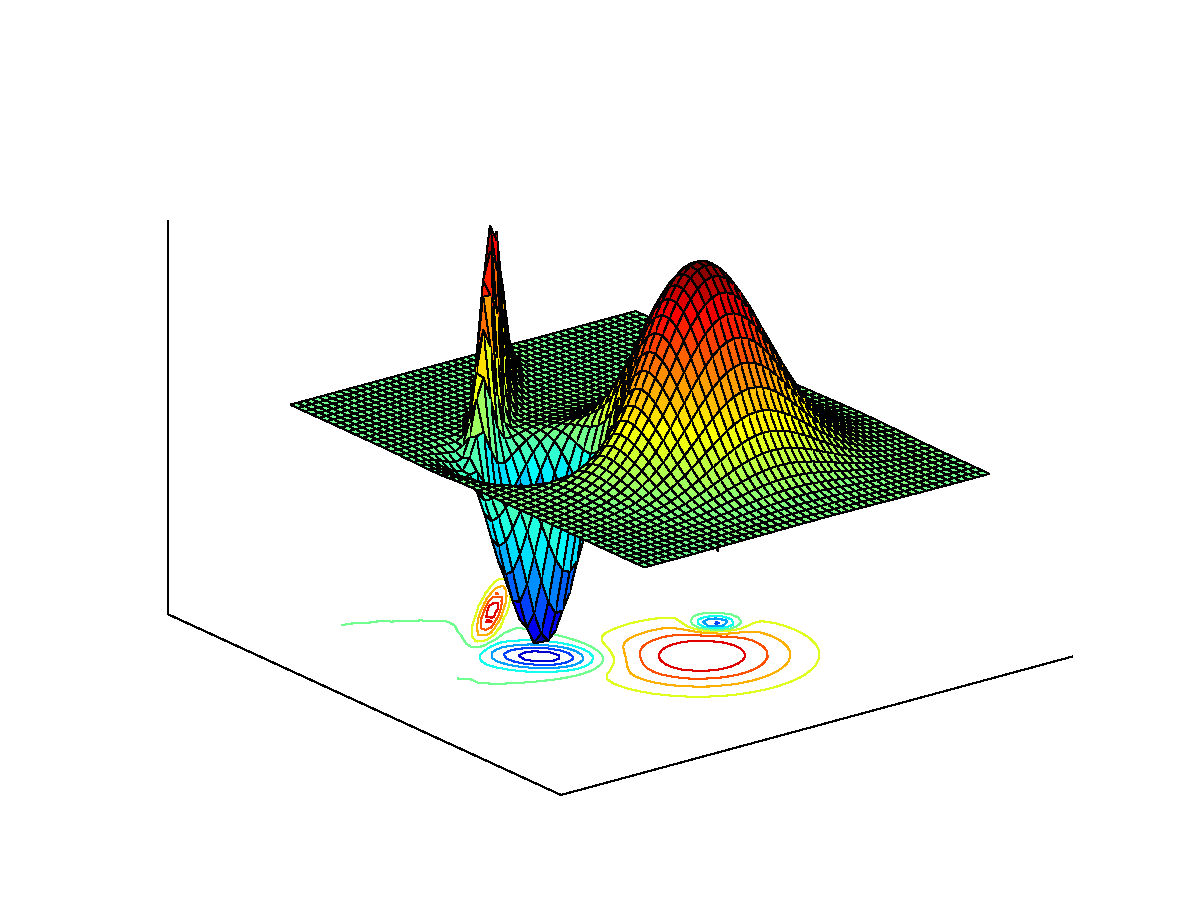
\includegraphics[width=\textwidth]{figures/surface.eps}
        \end{subfigure}
        ~
         \begin{subfigure}[b]{0.45\columnwidth}
                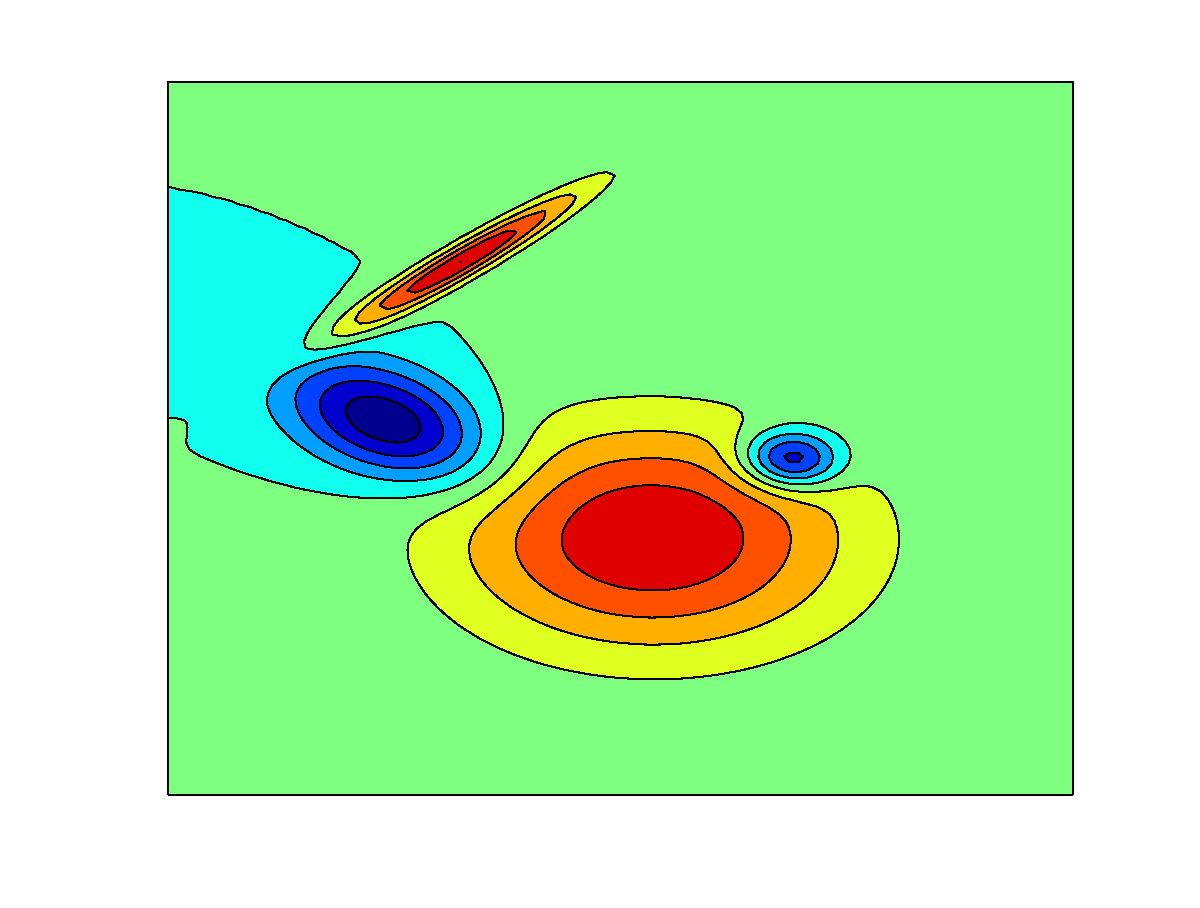
\includegraphics[width=\textwidth]{figures/contour.eps}
        \end{subfigure}
                       
        \caption{A toy regression problem generated from a mixture of random Gaussian kernels. }       
       \label{fig-toy-example}
\end{figure}

\begin{figure}
        \centering
        \begin{subfigure}[b]{0.3\columnwidth}
               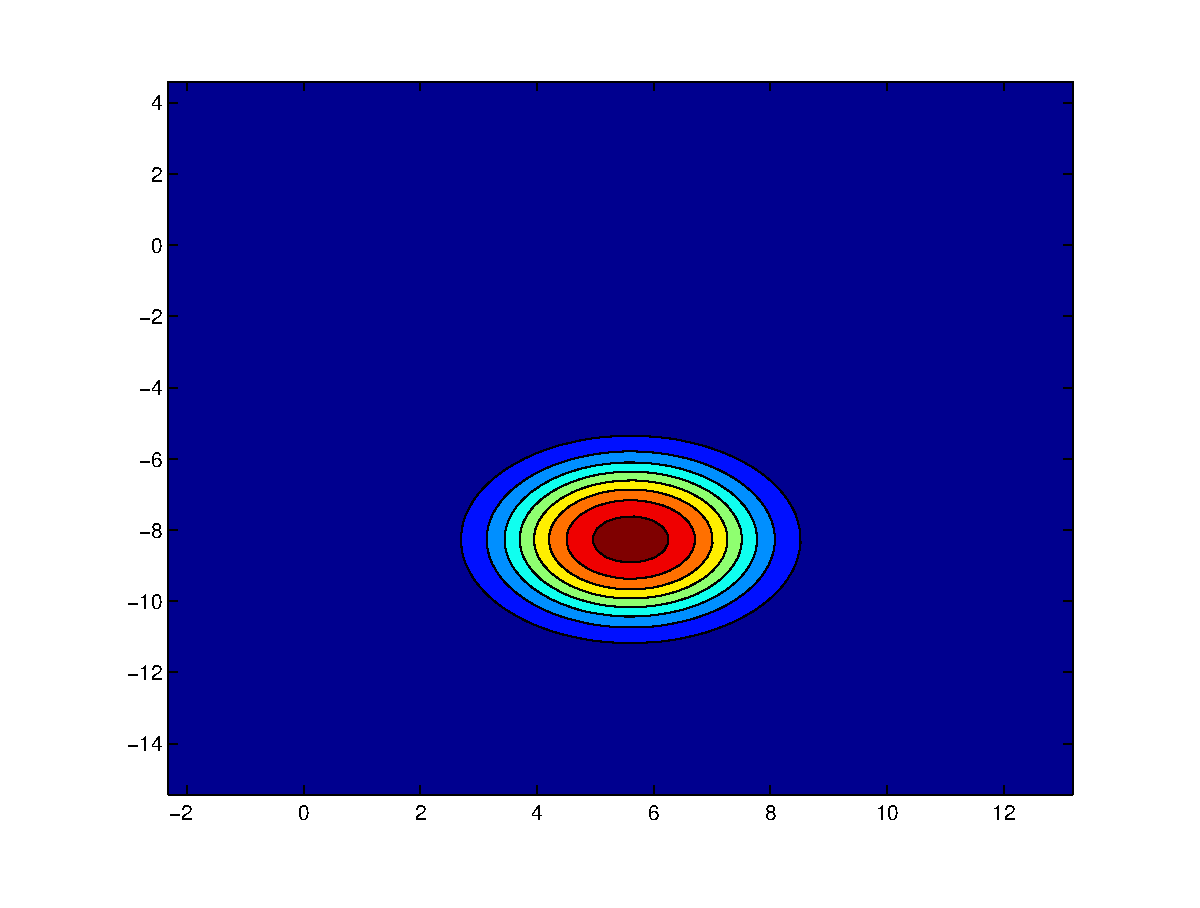
\includegraphics[width=\textwidth]{figures/GL1.eps}
        \end{subfigure}
        ~
         \begin{subfigure}[b]{0.3\columnwidth}
                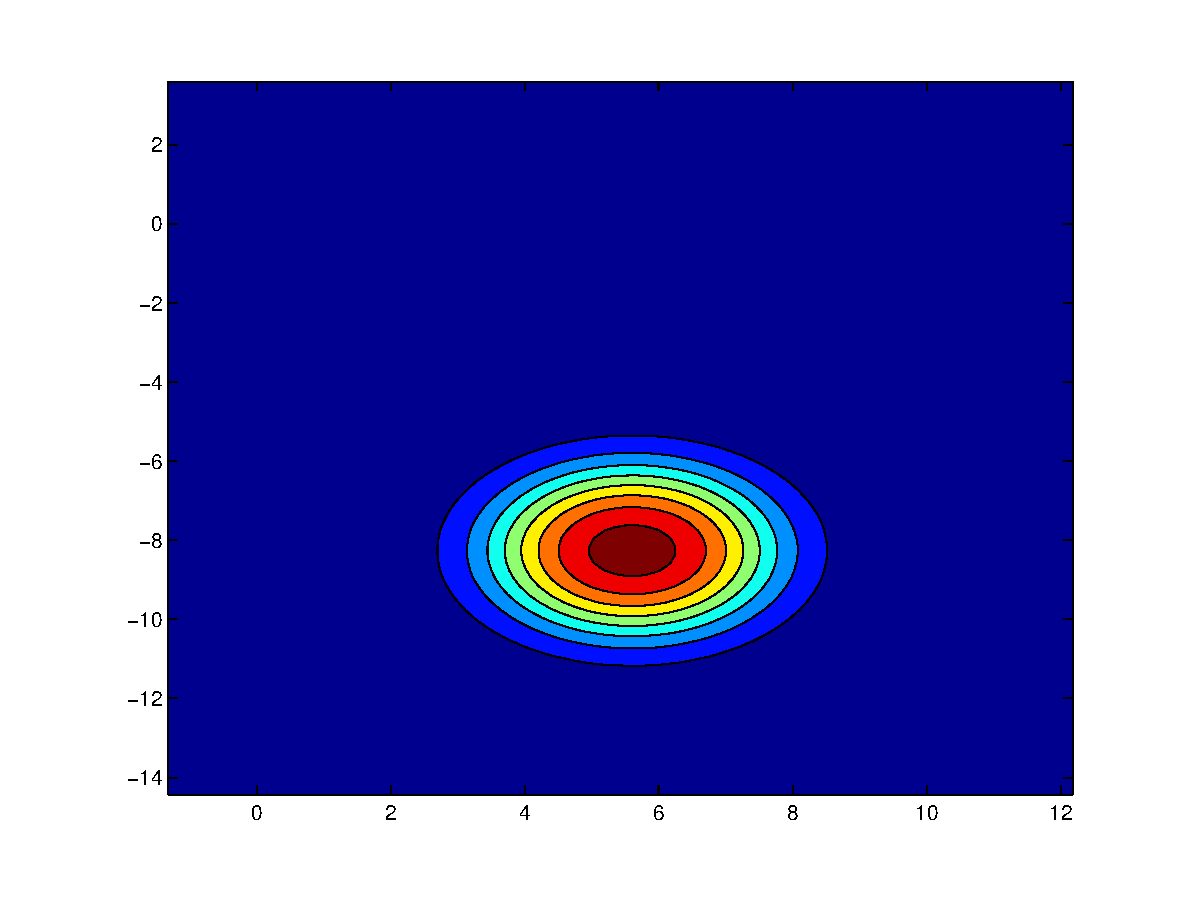
\includegraphics[width=\textwidth]{figures/VL1.eps}
        \end{subfigure}
        ~
        \begin{subfigure}[b]{0.3\columnwidth}
               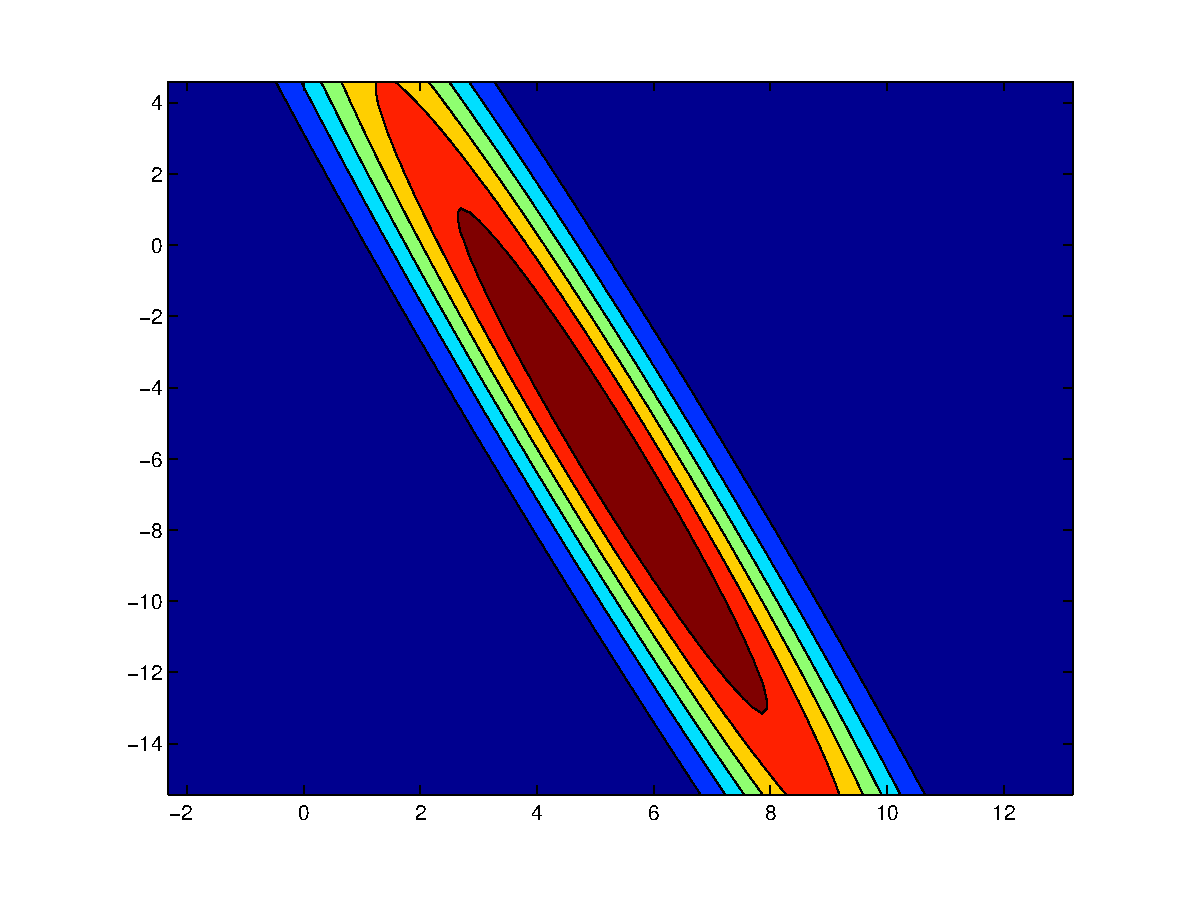
\includegraphics[width=\textwidth]{figures/VC1.eps}
        \end{subfigure}
       
         \begin{subfigure}[b]{0.3\columnwidth}
               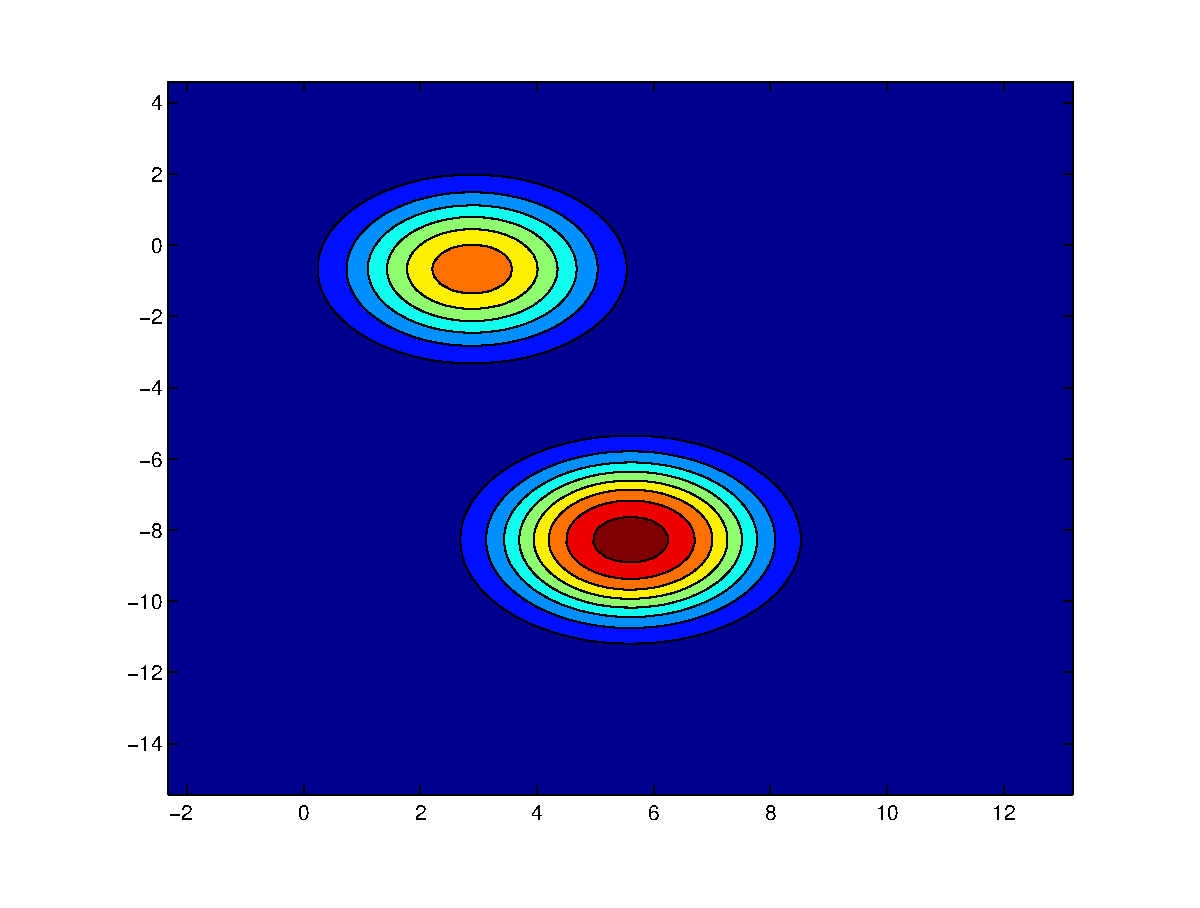
\includegraphics[width=\textwidth]{figures/GL2.eps}
        \end{subfigure}
        ~
         \begin{subfigure}[b]{0.3\columnwidth}
               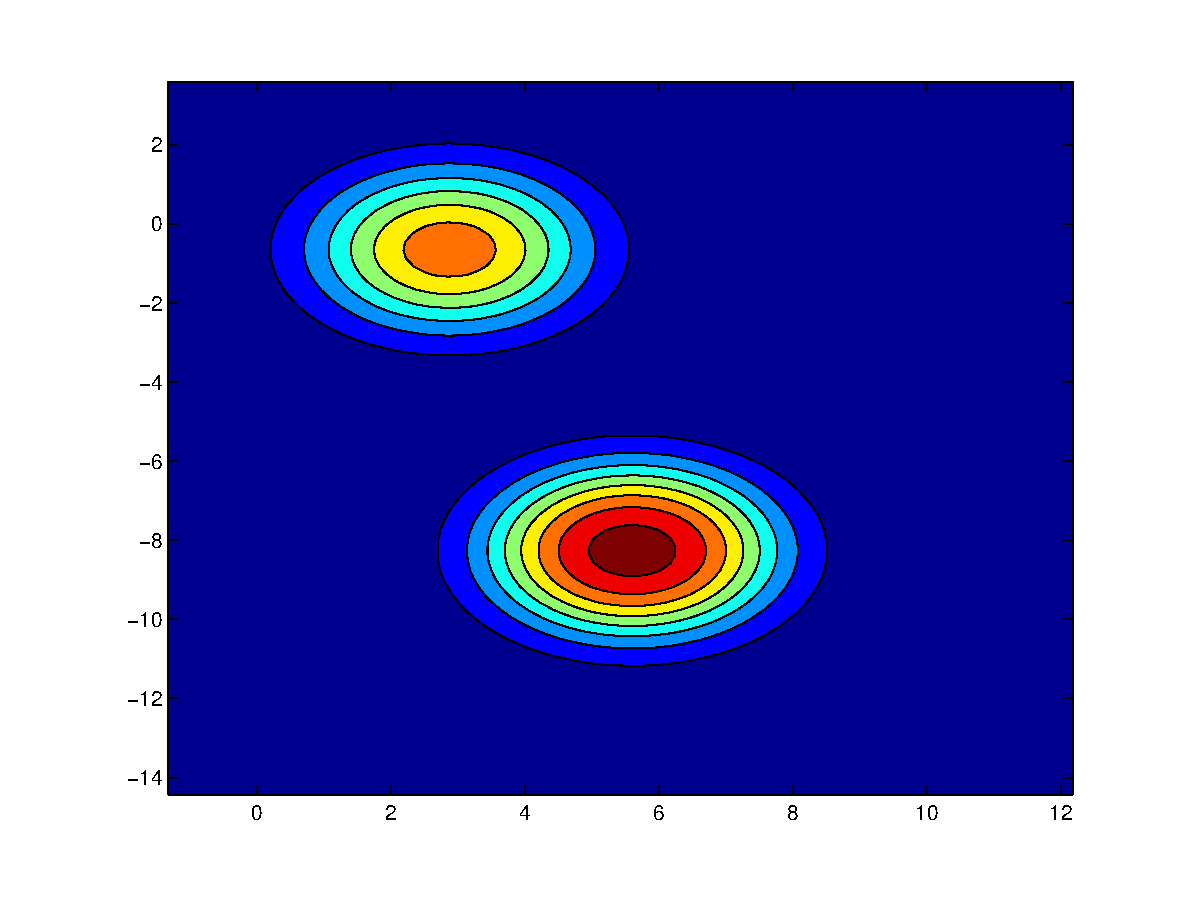
\includegraphics[width=\textwidth]{figures/VL2.eps}
        \end{subfigure}
        ~
        \begin{subfigure}[b]{0.3\columnwidth}
                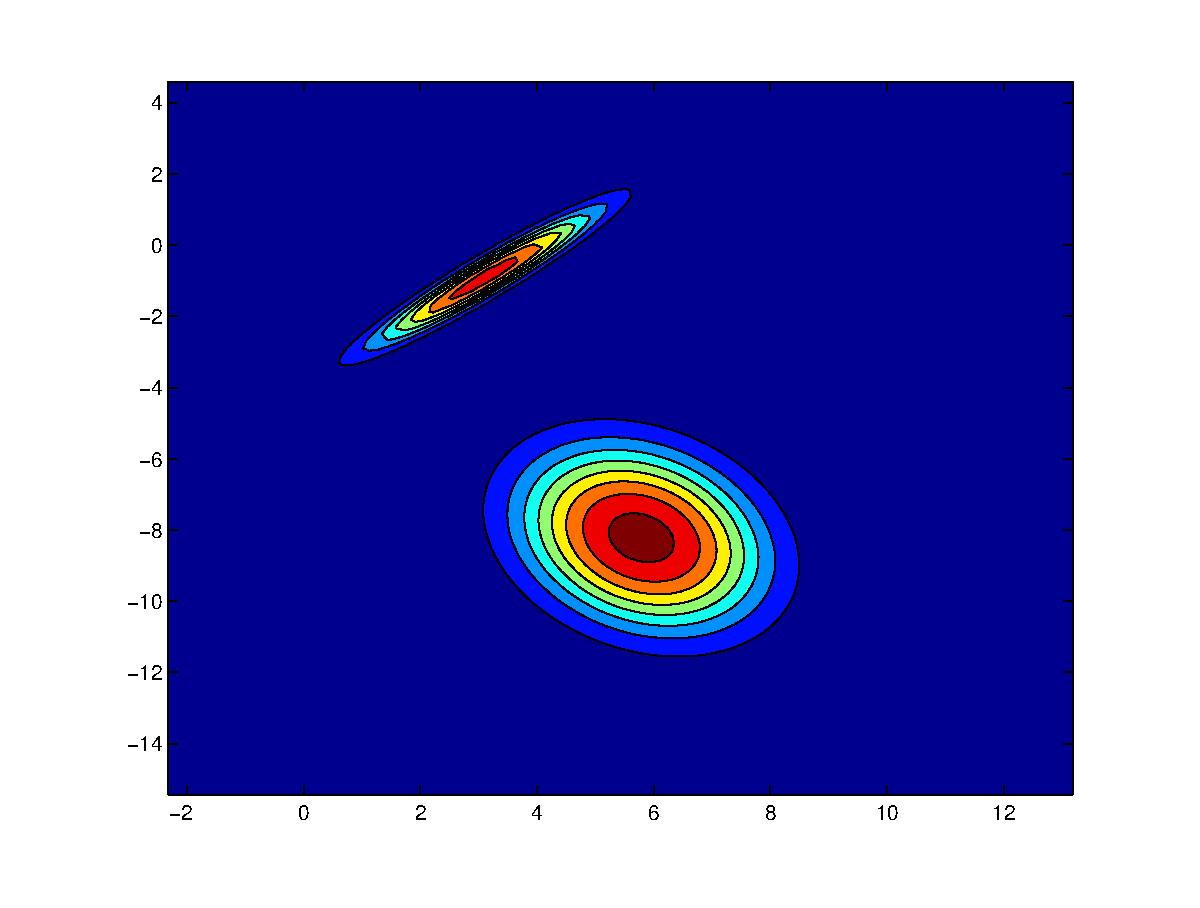
\includegraphics[width=\textwidth]{figures/VC2.eps}
        \end{subfigure}
       
         \begin{subfigure}[b]{0.3\columnwidth}
                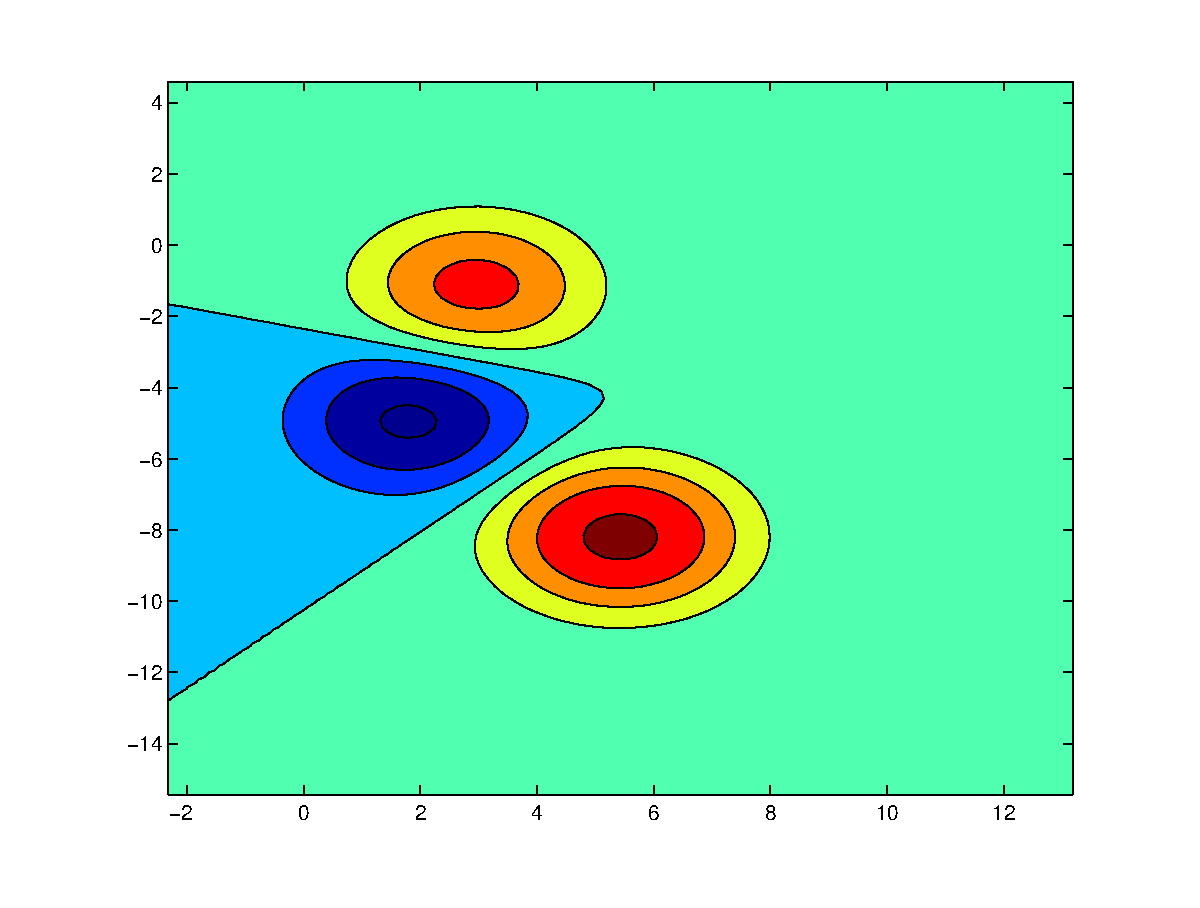
\includegraphics[width=\textwidth]{figures/GL3.eps}
        \end{subfigure}
        ~
         \begin{subfigure}[b]{0.3\columnwidth}
                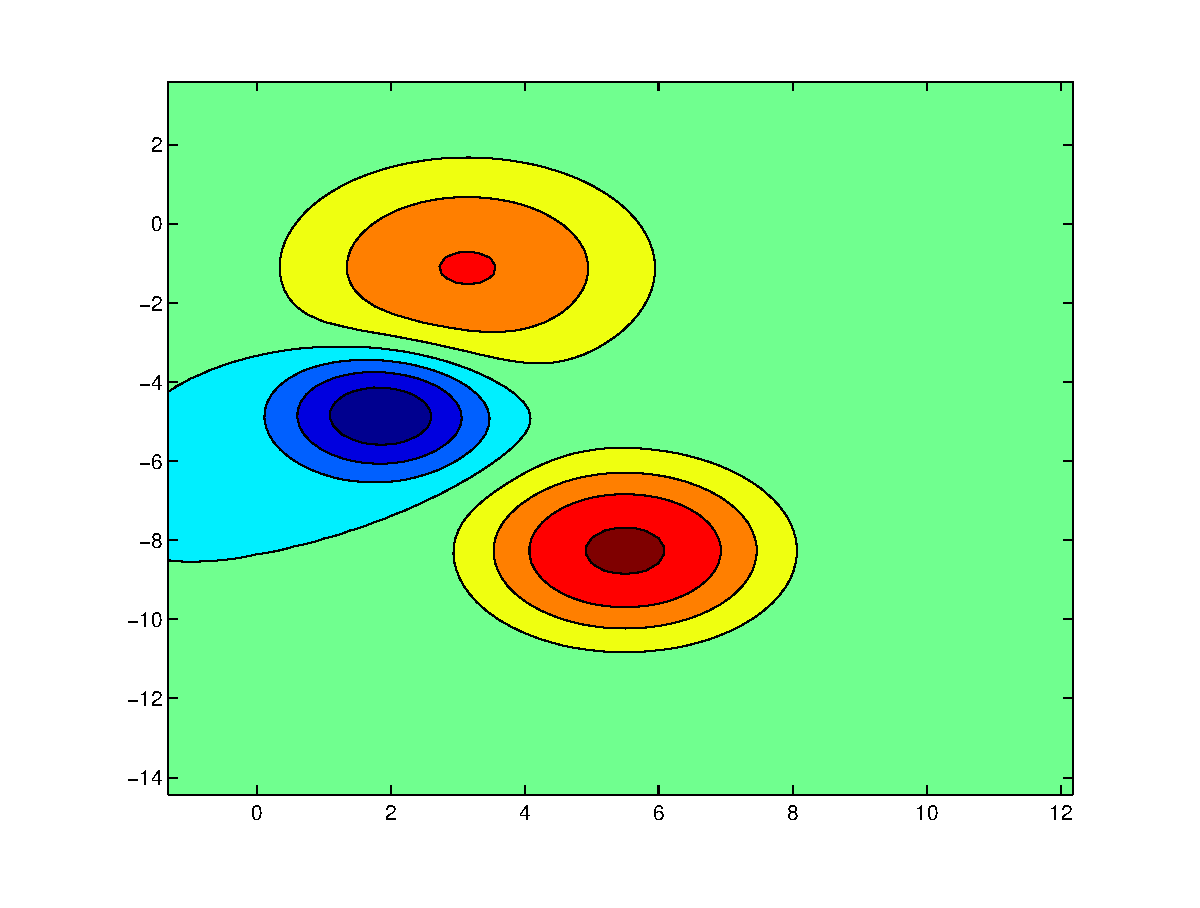
\includegraphics[width=\textwidth]{figures/VL3.eps}
        \end{subfigure}
        ~
        \begin{subfigure}[b]{0.3\columnwidth}
                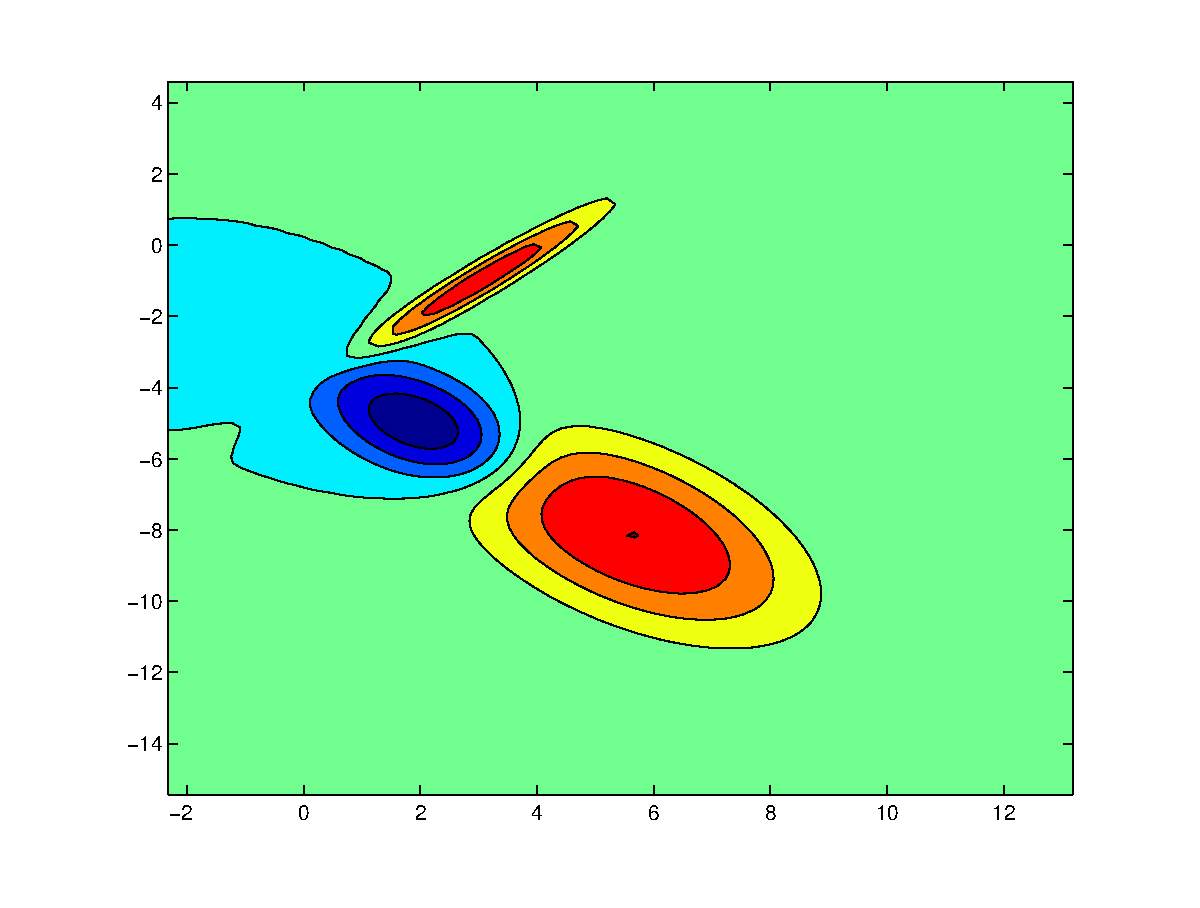
\includegraphics[width=\textwidth]{figures/VC3.eps}
        \end{subfigure}
       
         \begin{subfigure}[b]{0.3\columnwidth}
                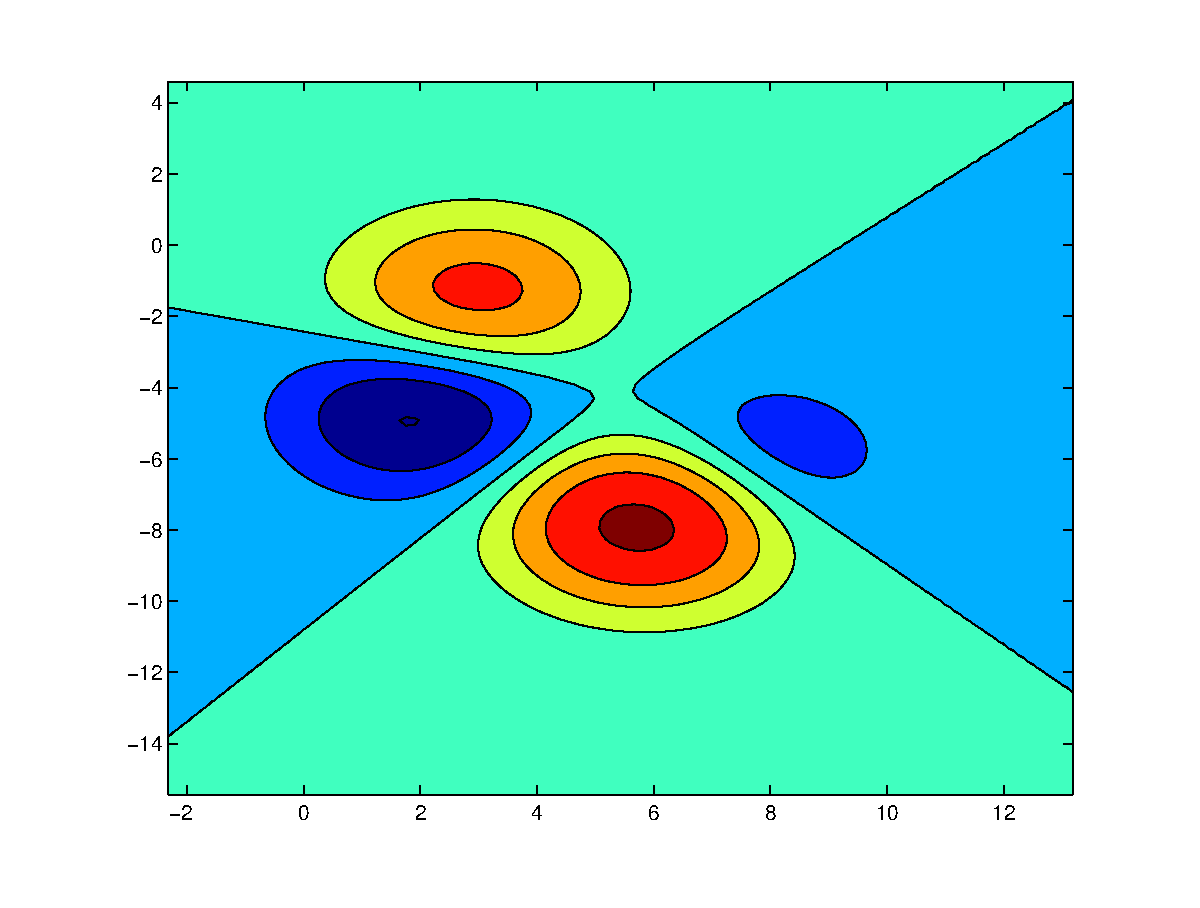
\includegraphics[width=\textwidth]{figures/GL4.eps}
                \caption{GP-GL}
        \end{subfigure}
        ~
         \begin{subfigure}[b]{0.3\columnwidth}
                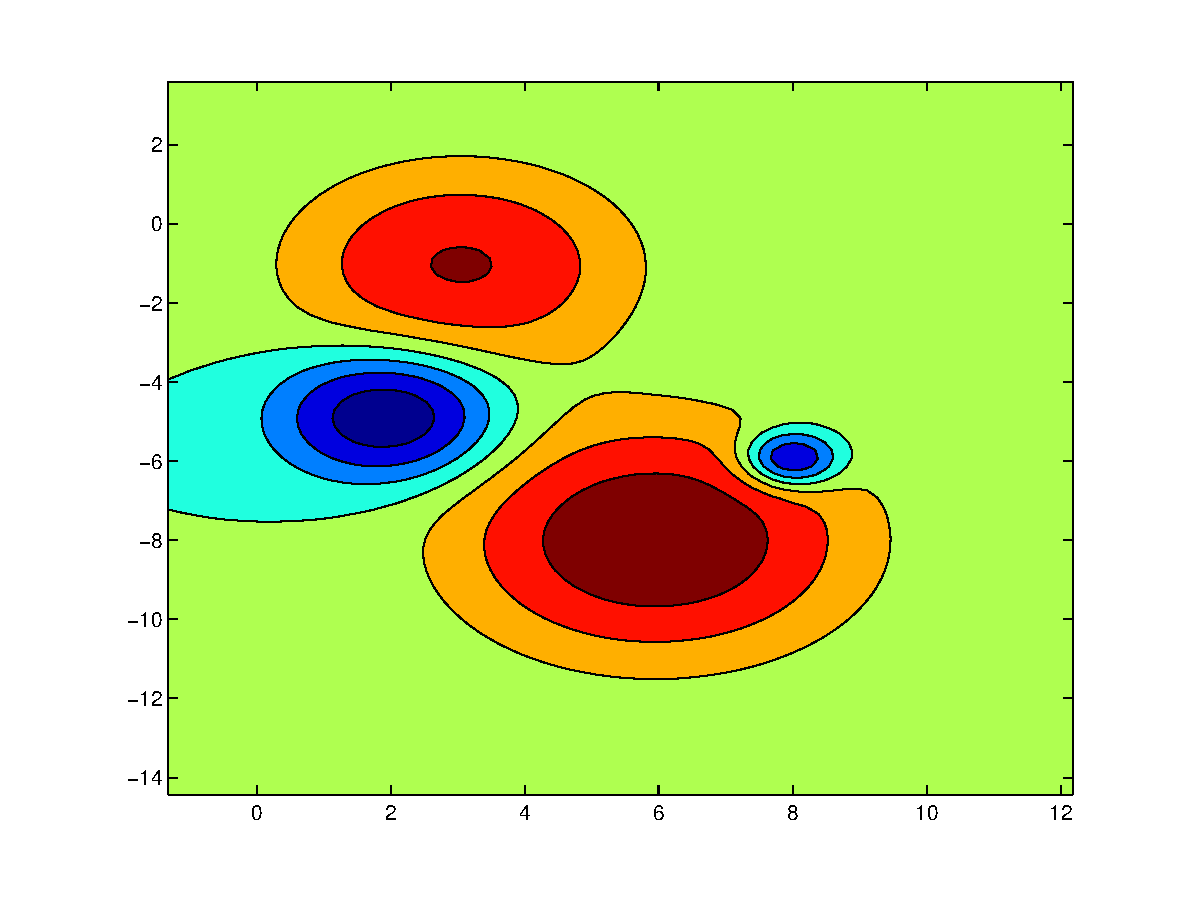
\includegraphics[width=\textwidth]{figures/VL4.eps}
                \caption{GP-VL}
        \end{subfigure}
        ~
        \begin{subfigure}[b]{0.3\columnwidth}
                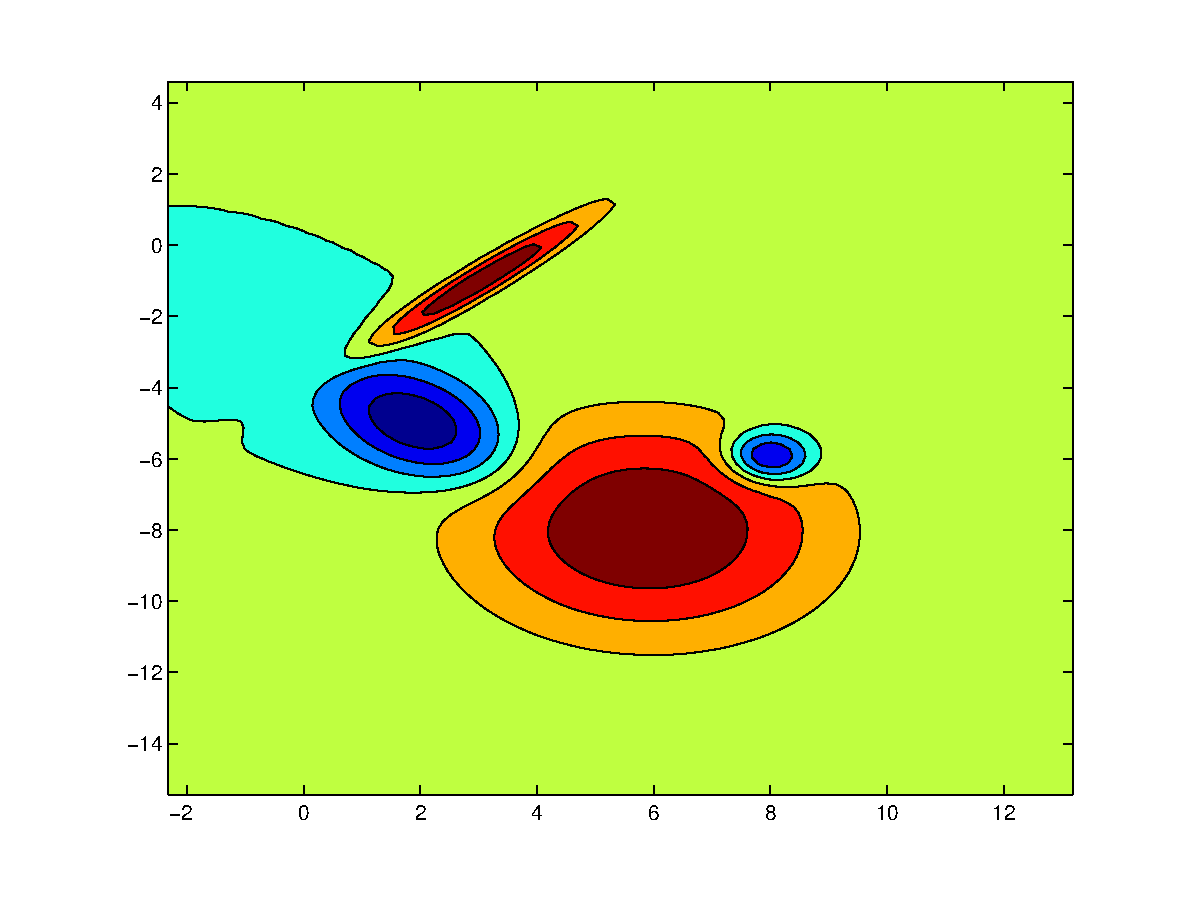
\includegraphics[width=\textwidth]{figures/VC4.eps}
                \caption{GP-VC}
        \end{subfigure}
               
        \caption{A comparisons between different sparse GP approaches with 1 to 4 basis functions (top to bottom) using (a) a global length scale, (b) variable length scales and (c) variable covariances }
        \label{fig-toy-comparison}
\end{figure}

\subsection{Linear Regression Prior}

GPs tend to perform well in interpolation but not as well in extrapolating. The regression function will fall back to the prior mean in areas where there is no training data. A common preprocessing technique is to subtract the mean of the output prior to training then adding it to the prediction of the model. Another way is to subtract a simple linear regression model and train the GP to learn the variation from that. This way, the GP will fall back to the linear regression prediction as a way of last resort instead of falling back to zero. We can incorporate this directly into the optimisation objective instead of having it as a separate preprocessing step by redefining $\bm{K}$ as a concatenation of the linear and non-linear features, or setting $\bm{K}=[\bm{K}|\bm{X}|\underset{n}{1}]$. Furthermore, the regularisation matrix in Eq. \eqref{eq-linear-regression-objective-rectangular} can be modified so that it penalises for learning high coefficients for the non-linear terms but no or little cost for learning linear terms by setting the corresponding elements in the diagonal of $I$ to 0, or the last $d+1$ elements. Therefore, as $\sigma_{n}^{2}$ goes to infinity, the model will get closer to a simple linear regression model.

\subsection{Cost Sensitive Learning}

So far the objective is to minimise the sum of squared errors, which is a suitable objective for most applications. However, this objective is naturally biased to the mean of the input and output distributions, therefore sacrificing data samples in less represented regions of the space. This is not always a desired effect, ideally we would like to train with well balanced data to avoid any bias, but this is a luxury that we often do not have. A common technique is to either over-sample or under-sample the data to achieve balance \citep{weiss2007}. In under-sampling, samples are removed from highly represented regions to achieve balance, over-sampling on the other hand duplicates under represented samples. Both approaches come with a cost, in the former good data is being wasted and in the latter more computation is introduced due to the data size increase. In this paper, we used what is known as cost-sensitive learning, which increases the error cost for low represented samples to mimic over-sampling balance. In classification tasks, a cost per sample is introduced such that the sum of the weights for each class are equal. In regression tasks, the output can be either discretised and treated as classes for the purpose of cost assignment, or a probability function is fitted to the output then samples are weighted in proportion to their inverse probability. After the weights have been assigned, they can be incorporated directly into the objective as follows:

\begin{equation}
\label{eq-weighted-linear-regression-objective}
\begin{array}{lcl}
\underset{w}{\text{min}} &\frac{1}{2}\left ( \bm{K}w-y \right )^{T} \bm{W}\left( \bm{K}w-y \right )+\frac{1}{2}\sigma_{n}^{2}w^{T}w
\end{array}
\end{equation}

The only difference between the objectives in Eq. \eqref{eq-linear-regression-objective} and Eq. \eqref{eq-weighted-linear-regression-objective} is the introduction of the diagonal matrix $\bm{W}$, where each element $\bm{W}_{ii}$ is the corresponding cost for sample $i$. The first term in Eq. \eqref{eq-weighted-linear-regression-objective} is a matrix form for a weighted sum of squares $\sum_{i=1}^{n}\bm{W}_{ii}\left(\bm{K}_{i,*}w-y_{i}\right)^{2}$, where the solution can be found analytically as follows:

\begin{equation}
\label{eq-weighted-linear-regression-objective-rectangular}
w = \left(\bm{K}^{T}\bm{WK}+\bm{I}\sigma_{n}^{2} \right)^{-1}\bm{K}^{T}\bm{W}y
\end{equation}

The only modification to the gradient calculation is to set the matrix $\bm{E}=\bm{W}\left(\left(\bm{K}w-y\right)w^{T}\right)\circ\bm{K}$.

\section{Application to Photometric Redshift Estimation}
\label{sec-application}

Here we consider the problem of redshift estimation from photometric data. The aim is to predict the spectroscopic redshift from the magnitudes of different colour bands omitted by a source using photometry, the light for each band is filtered to measure the magnitude of a certain wavelength range. We specifically target the photometric configuration designed for the Euclid Space Mission, namely the g, r, i, z, RIZ, Y, J and H bands and their associated expected errors. 

\subsection{Dataset}
\label{sec-dataset}

The dataset consist of the g, r, i, z, RIZ, Y, J and H magnitudes for 156,904 simulated sources along with their spectroscopic redshift. They cover a redshift range of $0.2 \le z_{spec} \le 2$ to target the requirement set by the Euclid Space Mission. All sources with any missing measurement in any of their detectors were removed prior to training. Not limits on any of the bands were used, although some will be explicitly removed to test the extrapolation performance of the models. The distribution of the bands and the spectroscopic redshift are provided in Figures \ref{fig-bands-histograms} and \ref{fig-zspec-hostogram} respectively. For all experiments reported in this paper, we ignore the error bars associated with each band and train only on the magnitudes. In all experiments reported in this paper, the data is preprocessed using Principle Component Analysis (PCA) \citep{jolliffe1986} to de-correlate the features prior to learning. De-correlation accelerates the convergence rate of the optimisation routine especially when using a logistic-type kernel machines like Neural Networks \citep{lecun1998}. To see this, consider a simple linear regression example where we would like to solve for $w$ in $Aw=b$, the solution for this is $w=\left(A^{T}A\right)^{-1}A^{T}b$. Note that if $A$ is de-correlated $A^{T}A=I$, therefore learning $w_{i}$ depends only on the $i$-th column of $A$ and it is independent from learning $w_{j}$, where $i\ne j$. In an optimisation approach, the convergence rate is a function of the condition of the $A^{T}A$ matrix, which is minimised in the case of de-correlated data. This essentially translate into a quadratic error surface which helps accelerate the search. An example of applying a simple coordinate-descent to optimise a linear regression model was applied to the toy data set and the results are shown in Figure \ref{fig-error-surface}.


\begin{figure*}
        \centering
        \begin{subfigure}[b]{0.15\textwidth}
                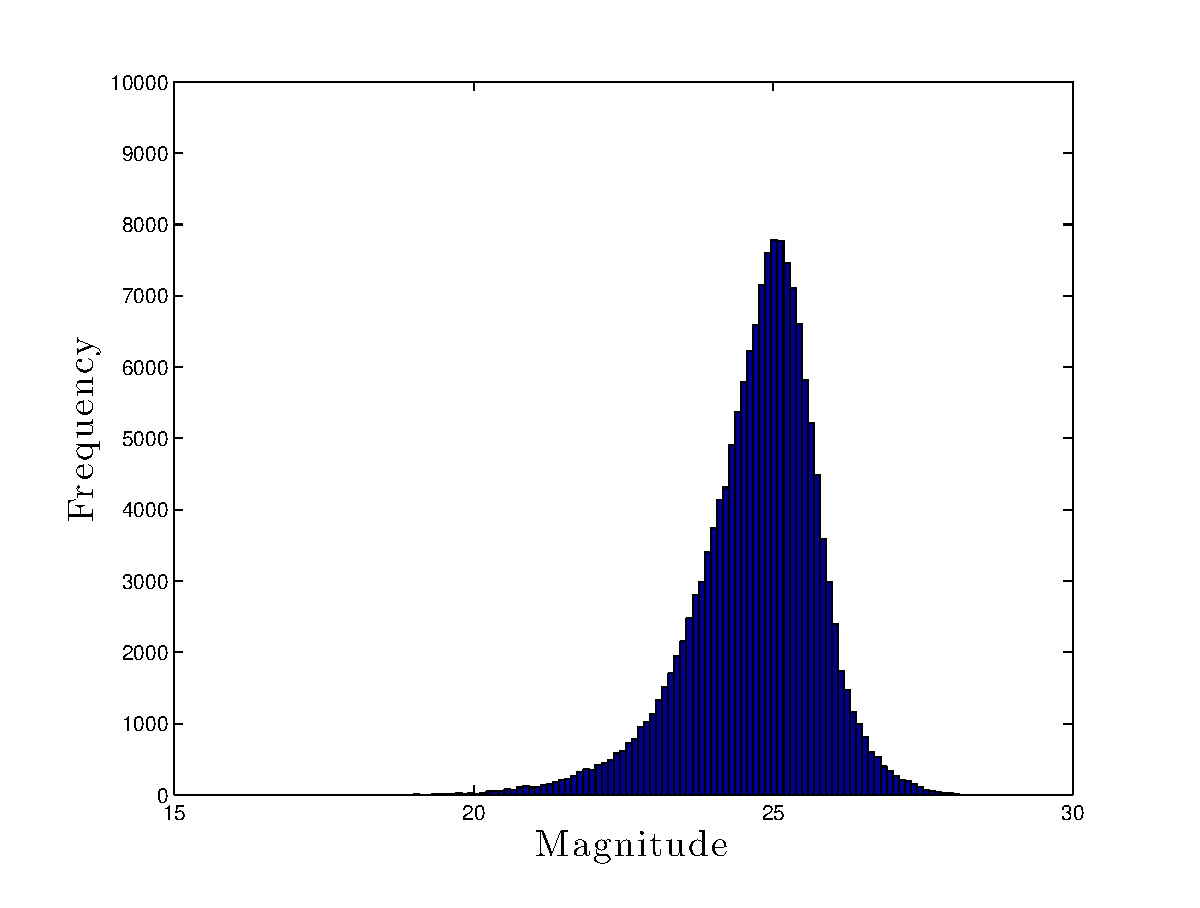
\includegraphics[width=\columnwidth]{figures/g.eps}
                \caption{g}
        \end{subfigure}
        ~
        \begin{subfigure}[b]{0.15\textwidth}
                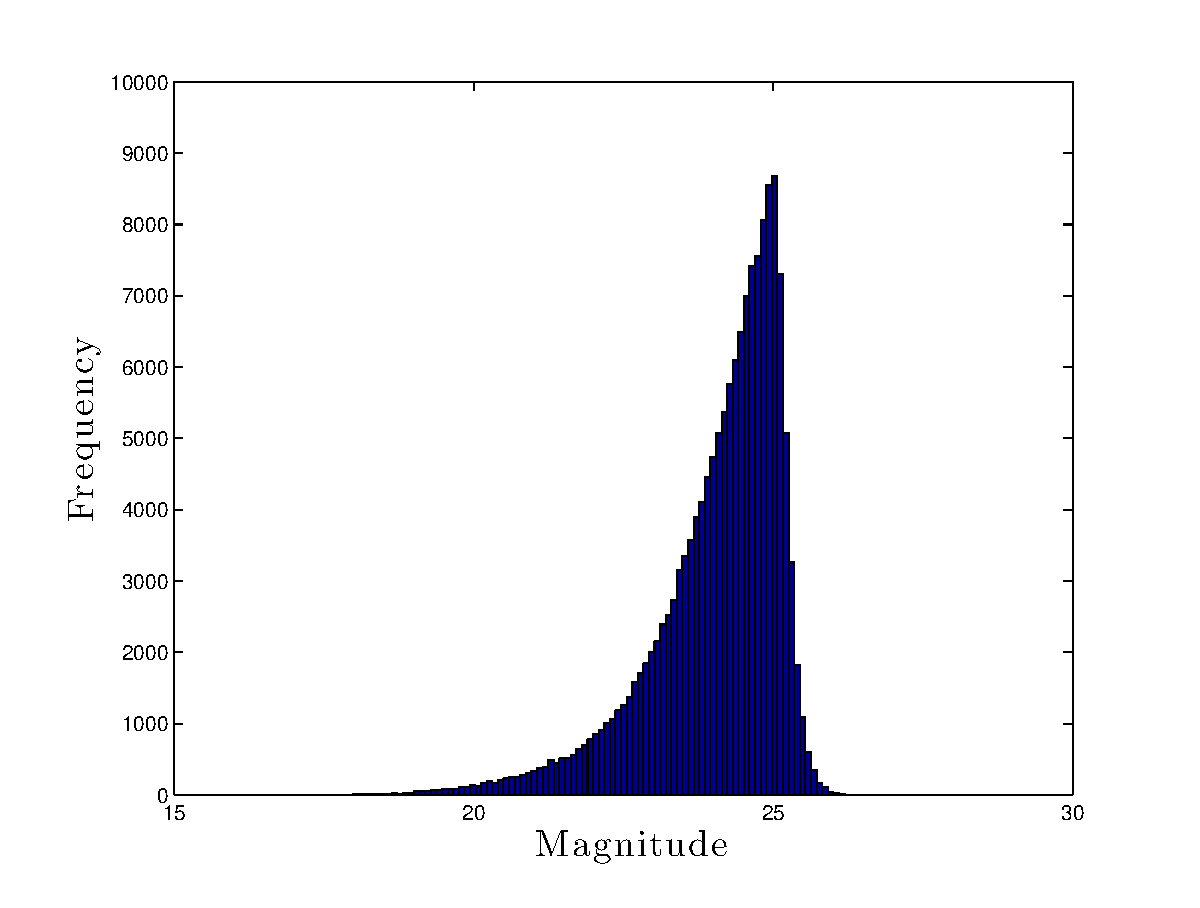
\includegraphics[width=\columnwidth]{figures/r.eps}
                \caption{r}
        \end{subfigure}
         ~
        \begin{subfigure}[b]{0.15\textwidth}
                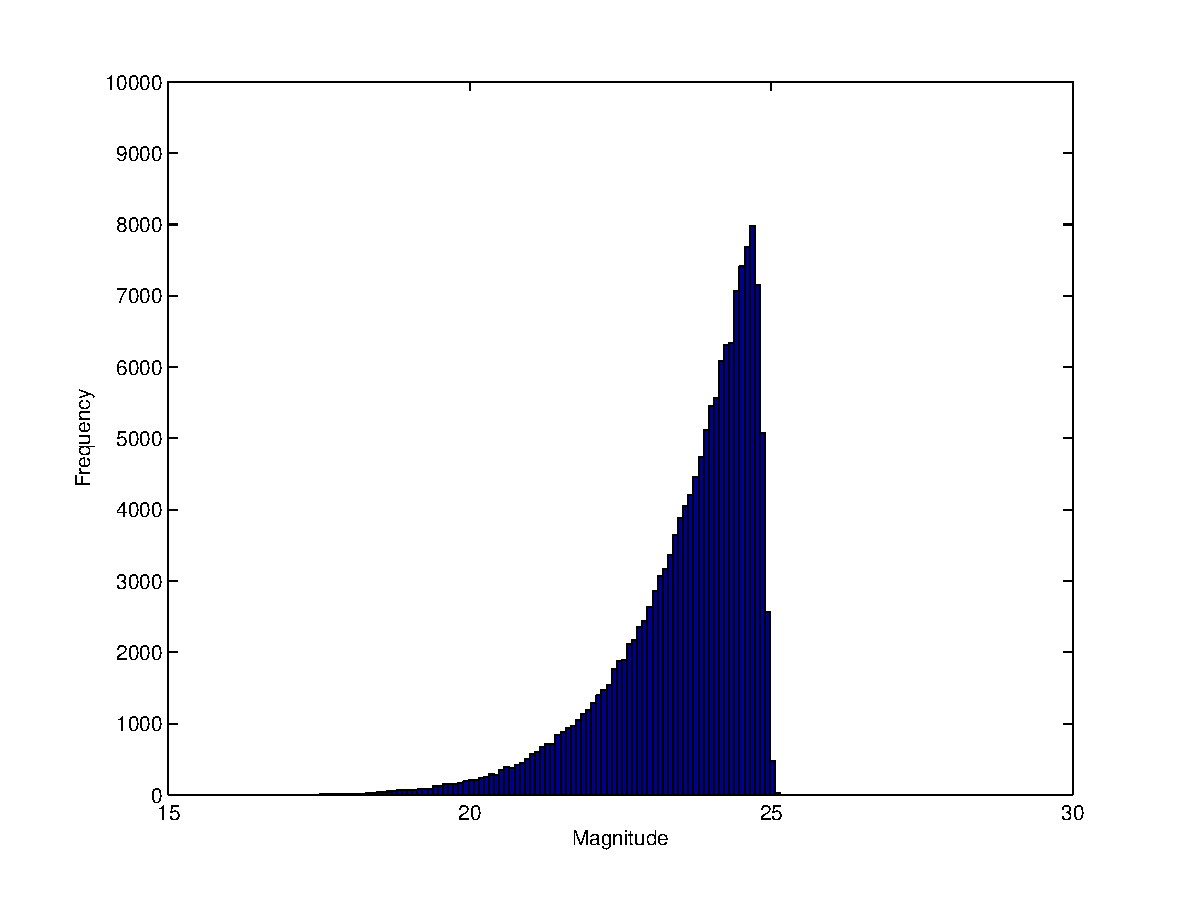
\includegraphics[width=\columnwidth]{figures/i.eps}
                \caption{i}
        \end{subfigure}
         ~
        \begin{subfigure}[b]{0.15\textwidth}
                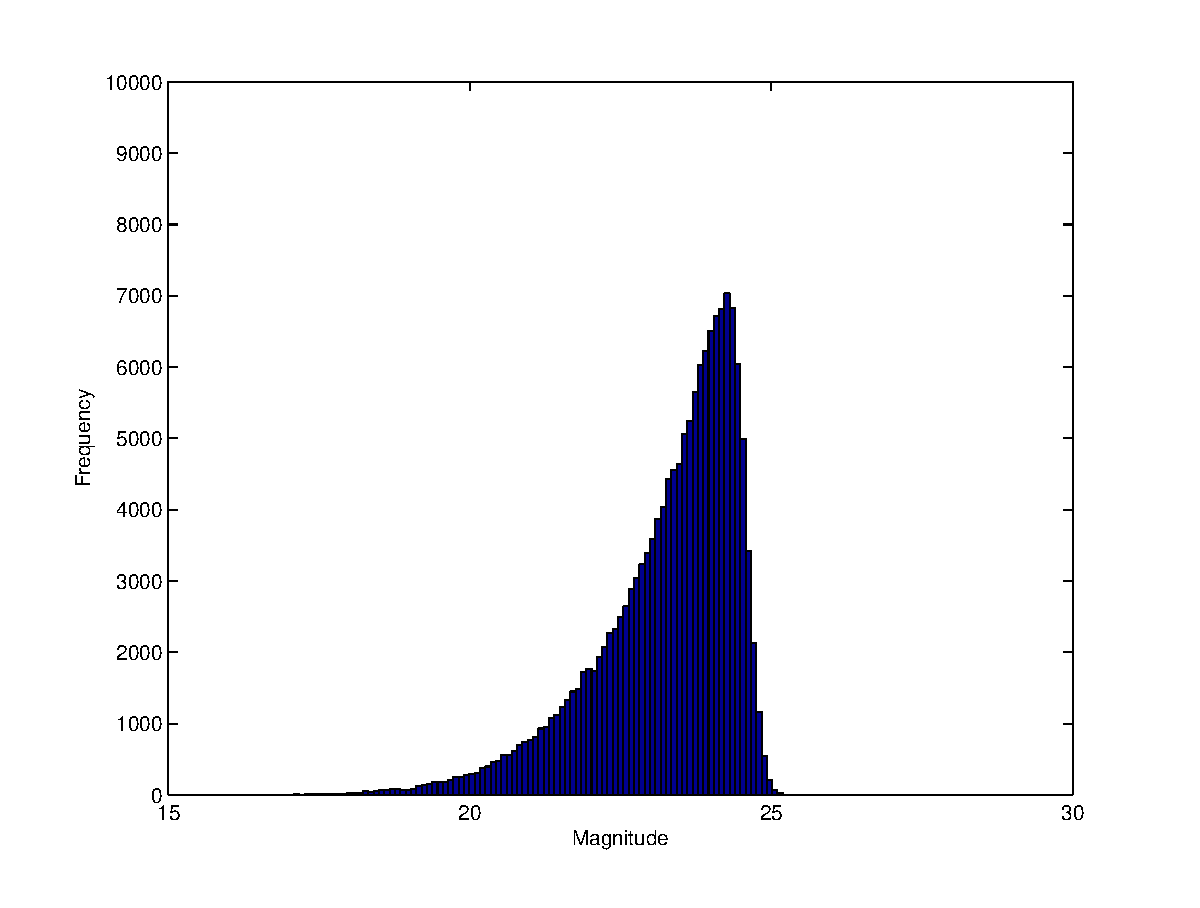
\includegraphics[width=\columnwidth]{figures/z.eps}
                \caption{z}
        \end{subfigure}
        
        \begin{subfigure}[b]{0.15\textwidth}
                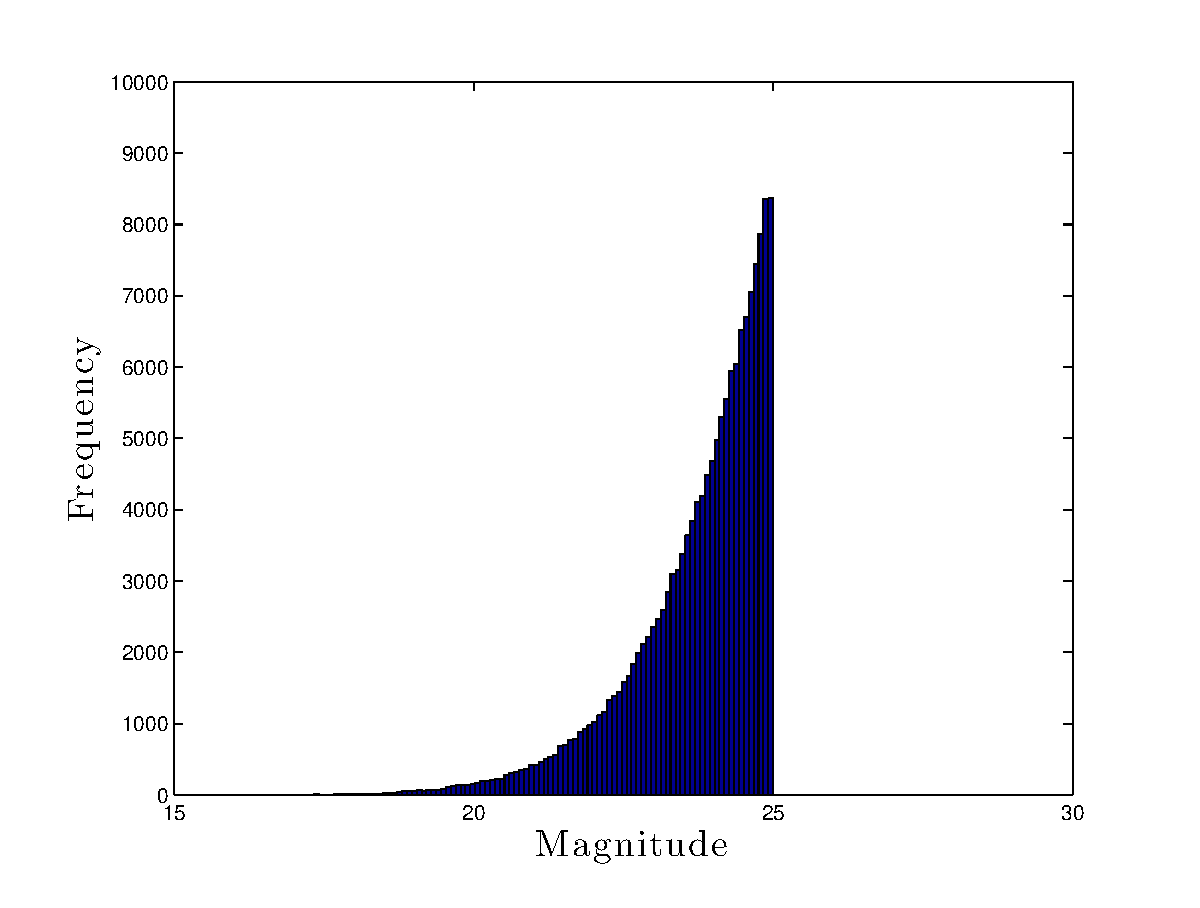
\includegraphics[width=\columnwidth]{figures/RIZ.eps}
                \caption{RIZ}
        \end{subfigure}
        ~
        \begin{subfigure}[b]{0.15\textwidth}
                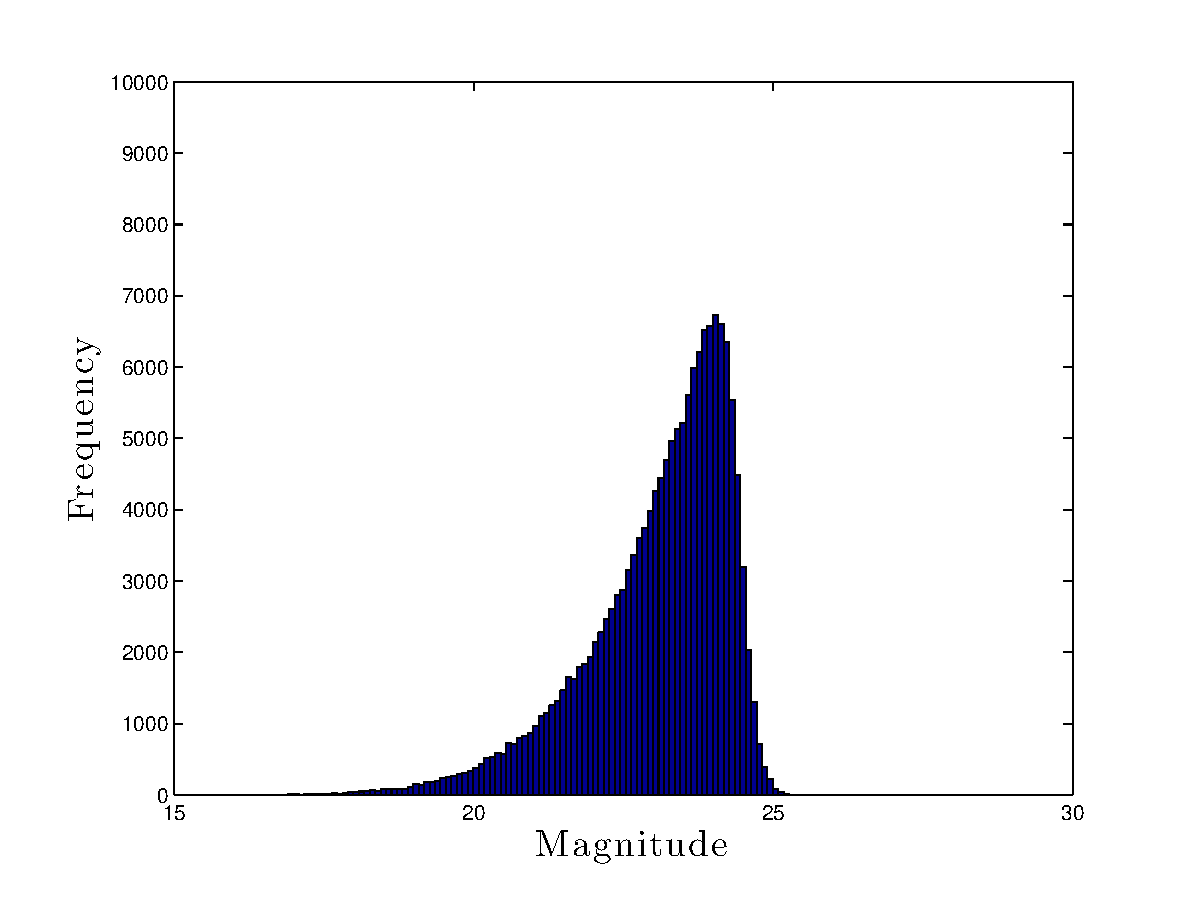
\includegraphics[width=\columnwidth]{figures/Y.eps}
                \caption{Y}
        \end{subfigure}
         ~
        \begin{subfigure}[b]{0.15\textwidth}
                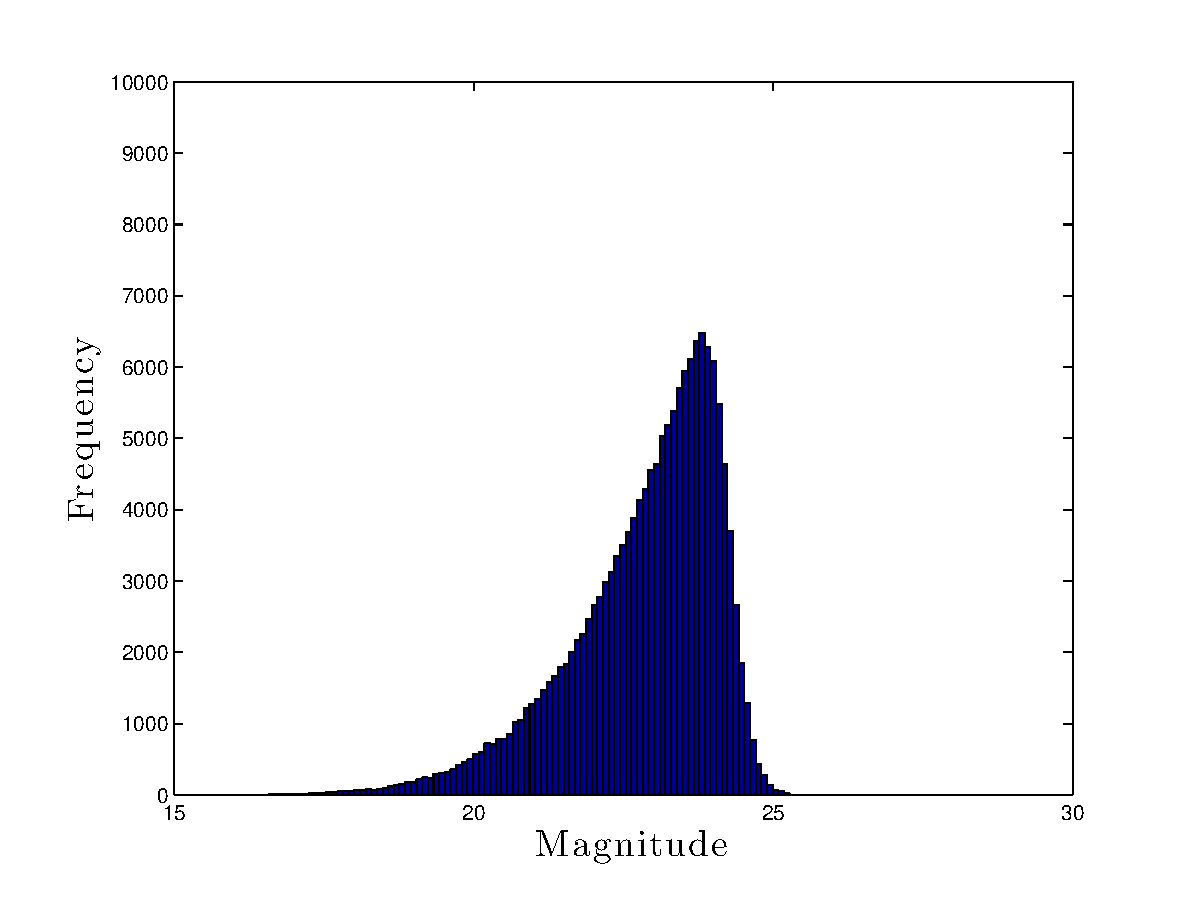
\includegraphics[width=\columnwidth]{figures/J.eps}
                \caption{J}
        \end{subfigure}
         ~
        \begin{subfigure}[b]{0.15\textwidth}
                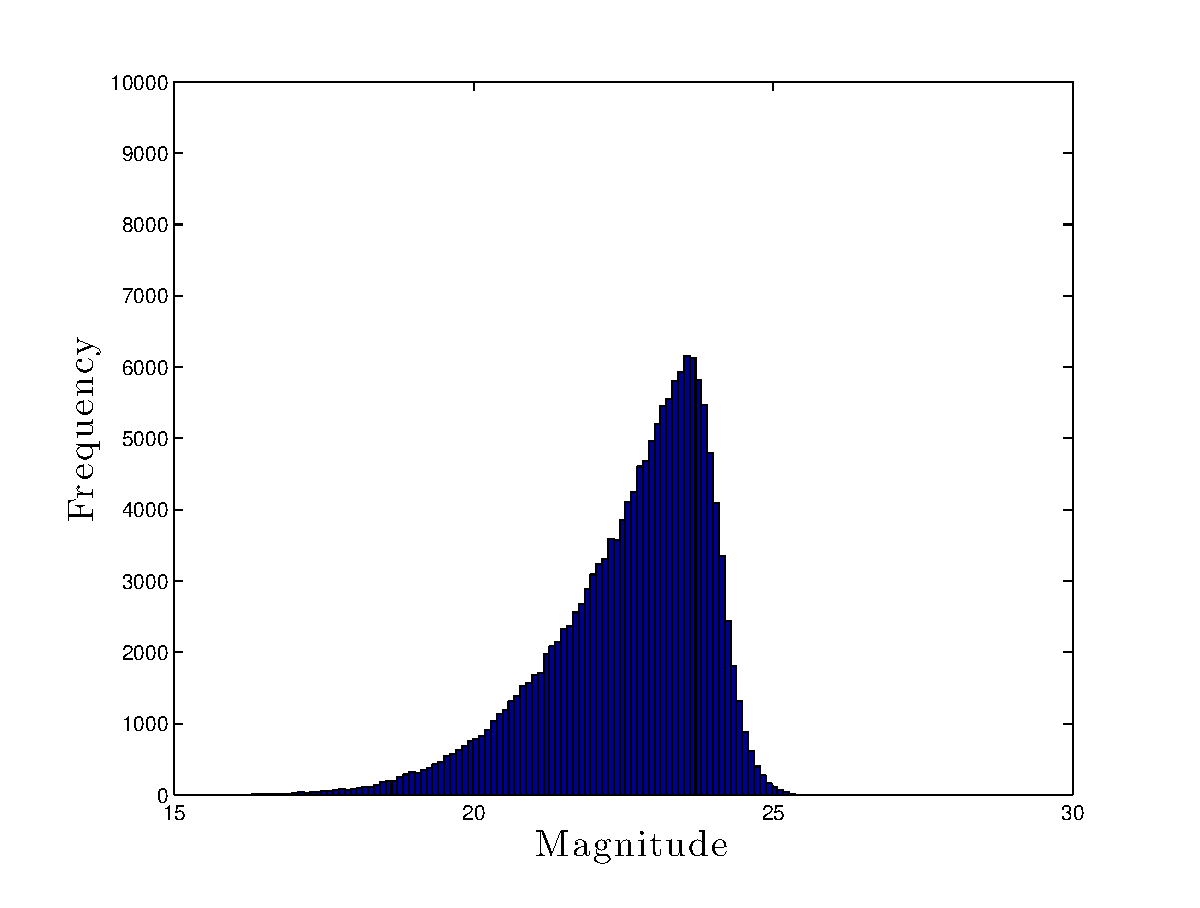
\includegraphics[width=\columnwidth]{figures/H.eps}
                \caption{H}
        \end{subfigure}
        
       \caption{The magnitude distribution for each band in the dataset.} 
	\label{fig-bands-histograms}
\end{figure*}

\begin{figure}
        \centering
        \begin{subfigure}[b]{0.45\columnwidth}
                 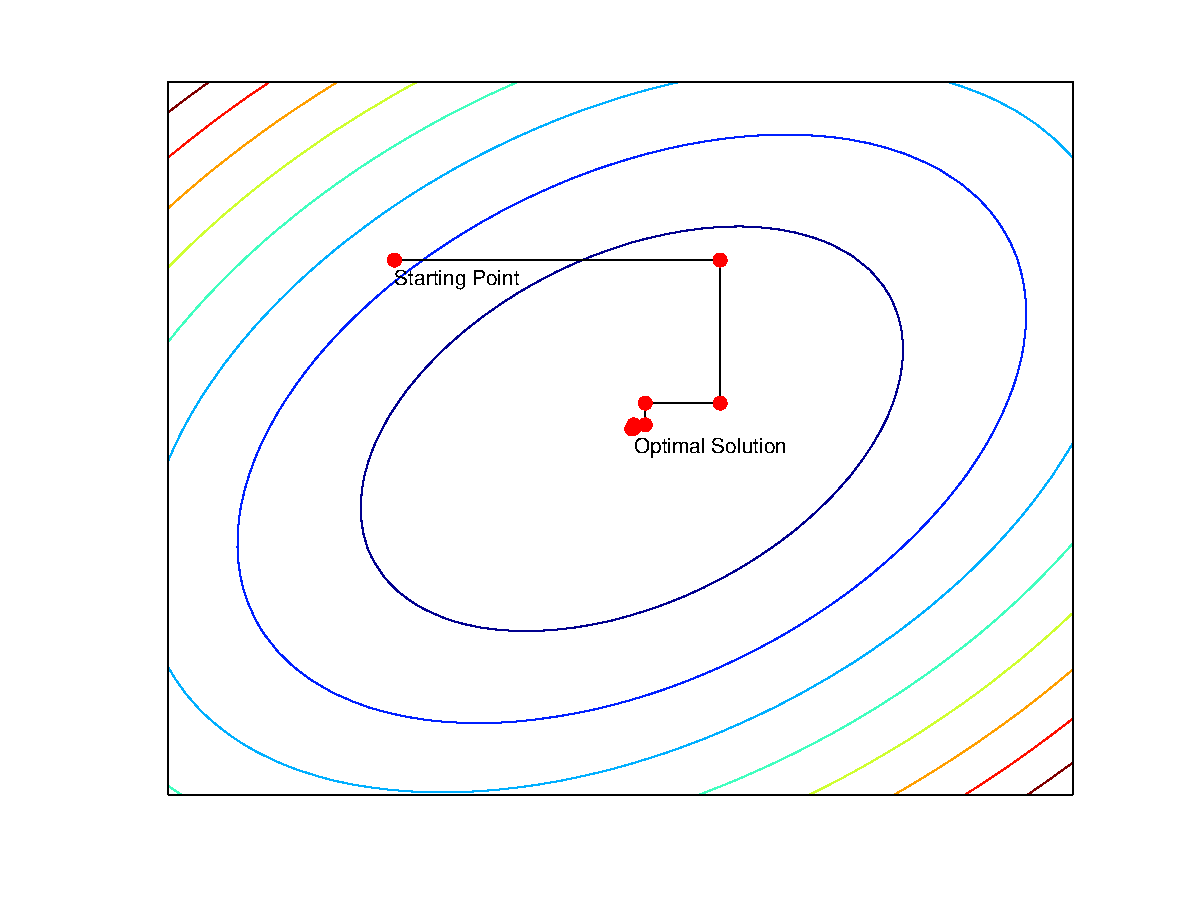
\includegraphics[width=\textwidth]{figures/correlated.eps}
                 \caption{Correlated}
        \end{subfigure}
        ~
        \begin{subfigure}[b]{0.45\columnwidth}
                 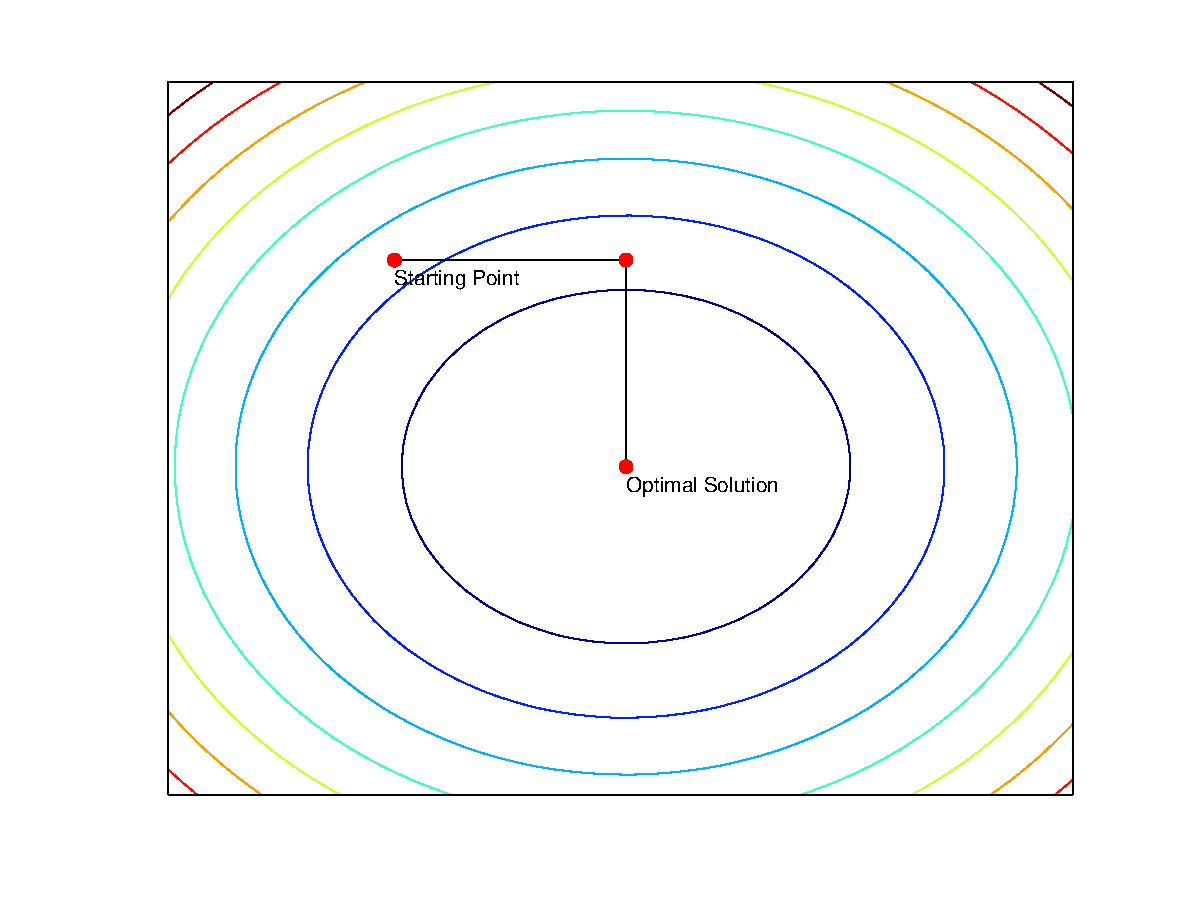
\includegraphics[width=\textwidth]{figures/decorrelated.eps}
                 \caption{De-correlated}
        \end{subfigure}
       \caption{Using coordinate-descent to optimise the linear regression objective on the toy dataset shown in Figure \ref{fig-toy-example}. Subfigure (a) shows the steps taken when the data has some correlation, while subfigure (b) shows the steps taken when the data was de-correlated.} 
	\label{fig-error-surface}
\end{figure}

\begin{figure}
       \centering
       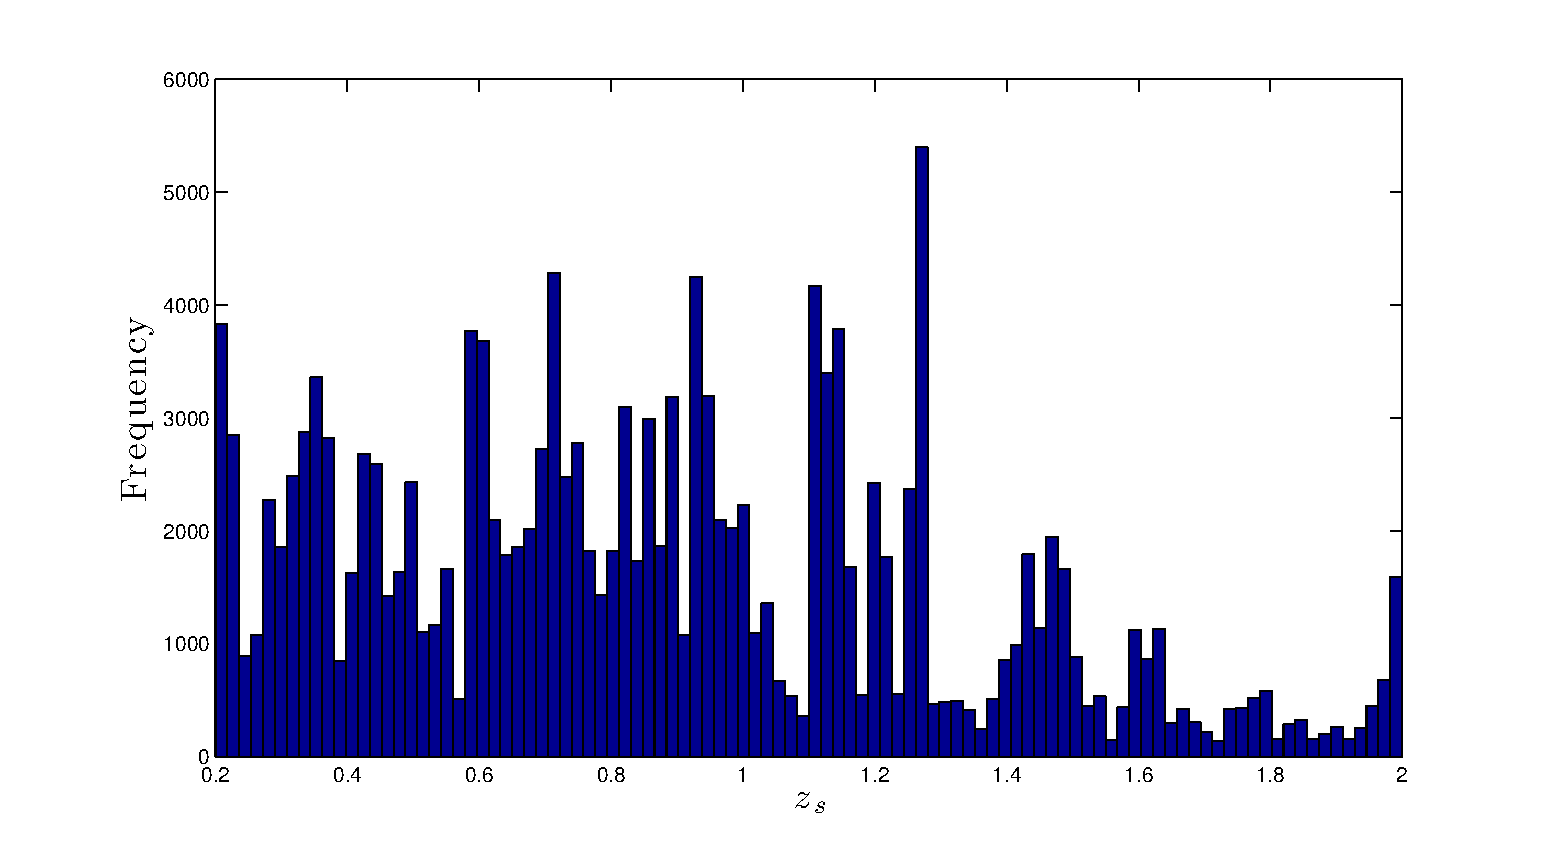
\includegraphics[width=\columnwidth]{figures/zspec.eps}
        \caption{The spectroscopic redshift distribution in the dataset.} 
       \label{fig-zspec-hostogram}
\end{figure}

\section{Experiments and Results}
\label{sec-experiments}

Five algorithms are considered to model the data, Artificial Neural Networks (ANN), GP with low rank approximation or stableGP , sparse GP with global length scale (GP-GL), GP with variable length scale (GP-VL) and  GP with variable covariances (GP-VC). For ANN, a single layer network is used with hyperbolic tangent hidden activations and linear output activations, for low rank approximation we use the SR-VP method proposed in \citep{foster2009}. In subsequent tests, the variable $m$ refers to the number of hidden units in ANN, the rank in stableGP, and the number of basis functions in GP-GL, GP-VL and GP-VC. The data was split into \%90 for training and \%10 for testing, the following performance measures on the test set are reported for each experiment:

\begin{itemize}
  \item $\Delta z_{\phantom{norm}} = \sqrt{\frac{1}{n}\sum_{i=1}^{n}\left(z_{spec}-z_{phot}\right)^{2}}$
  \item $\Delta z_{norm} = \sqrt{\frac{1}{n}\sum_{i=1}^{n}\left(\frac{z_{spec}-z_{phot}}{1+z_{spec}}\right)^{2}}$
\end{itemize}

$\Delta z$ is the standard Root Mean Squared Error (RMSE), while $\Delta z_{norm}$ is a normalised version that weighs low redshift objects more aggressively than higher redshift objects. The scientific goal of the Euclid mission is to reach a $\Delta z_{norm} \le 0.05$

\subsection{Modelling Performance}

In the first test, all models were trained using a fixed $m=10$ to cross compare the performance of the methods using the same number of basis functions. The number of basis was set deliberately low to highlight the modelling capabilities of each algorithm, as for large values of $m$ the performance gap between the algorithms is very small to distinguish the difference. The standard sum of squares objective was used, without cost sensitive training or a prior mean function. The $z_{spec}$ vs $z_{phot}$ density scatter plots are shown in Figure \ref{fig-experiment-1} and their performance scores are reported in Table \ref{table-experiment-1}

\begin{figure*}
        \centering
        \begin{subfigure}[b]{0.175\textwidth}
                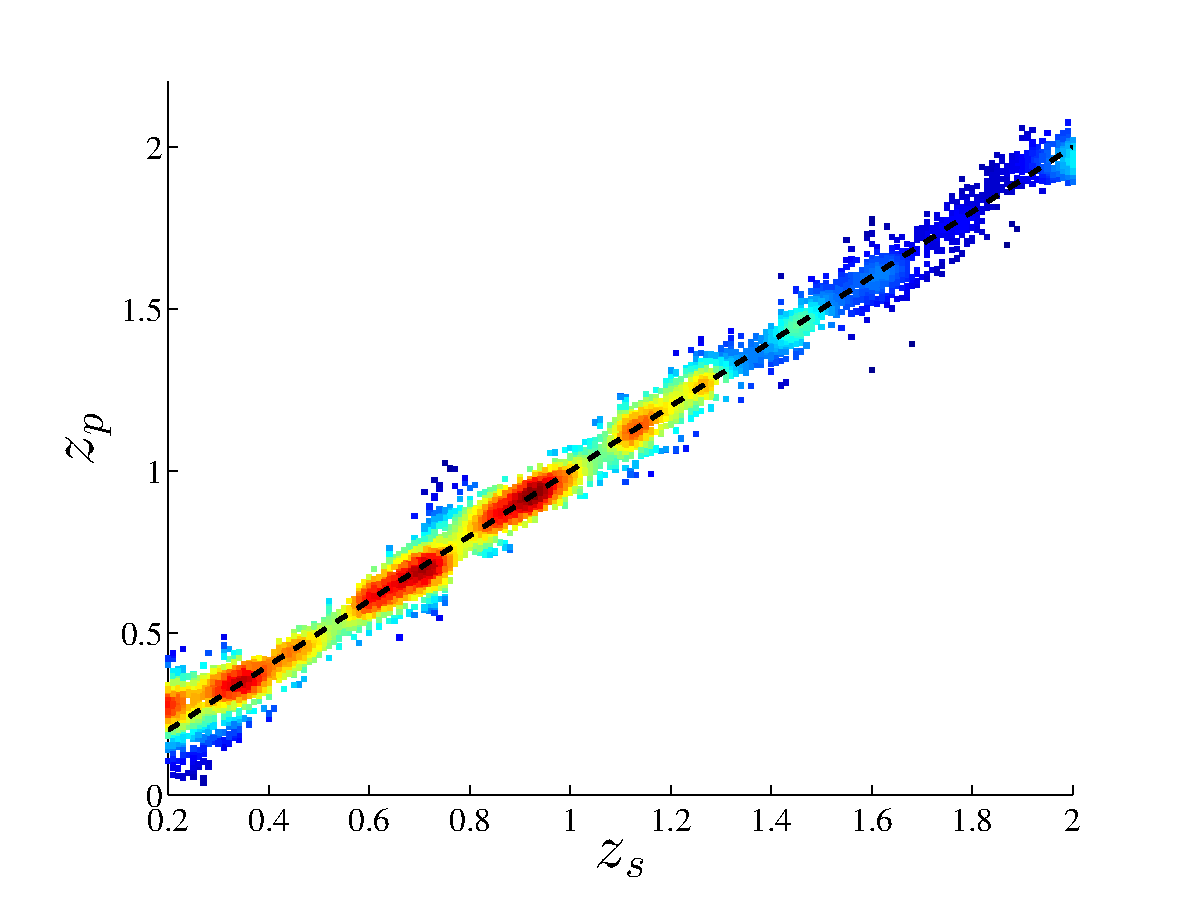
\includegraphics[width=\textwidth]{figures/ANN.eps}
                \caption{ANN}
        \end{subfigure}
        ~
        \begin{subfigure}[b]{0.175\textwidth}
                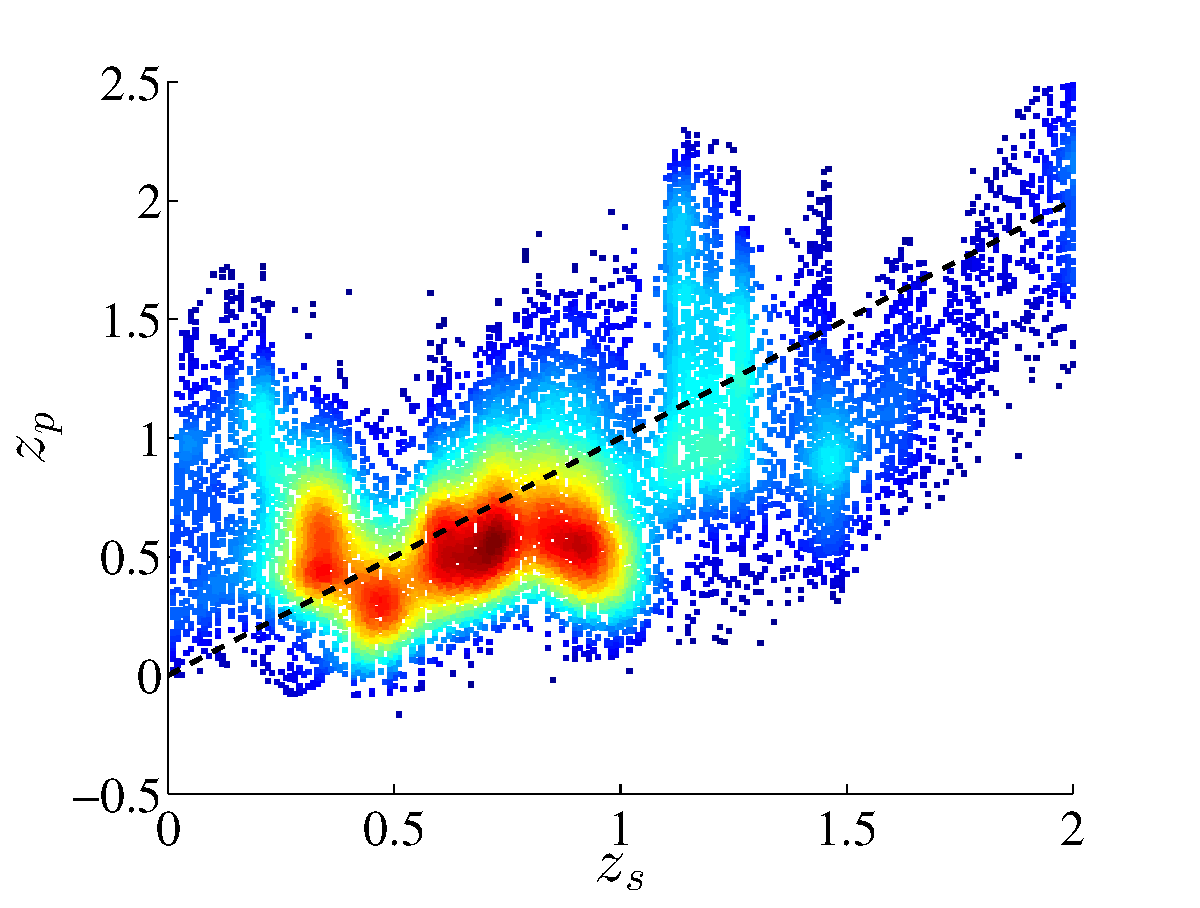
\includegraphics[width=\textwidth]{figures/stableGP.eps}
                \caption{stableGP}
        \end{subfigure}
        ~
        \begin{subfigure}[b]{0.175\textwidth}
                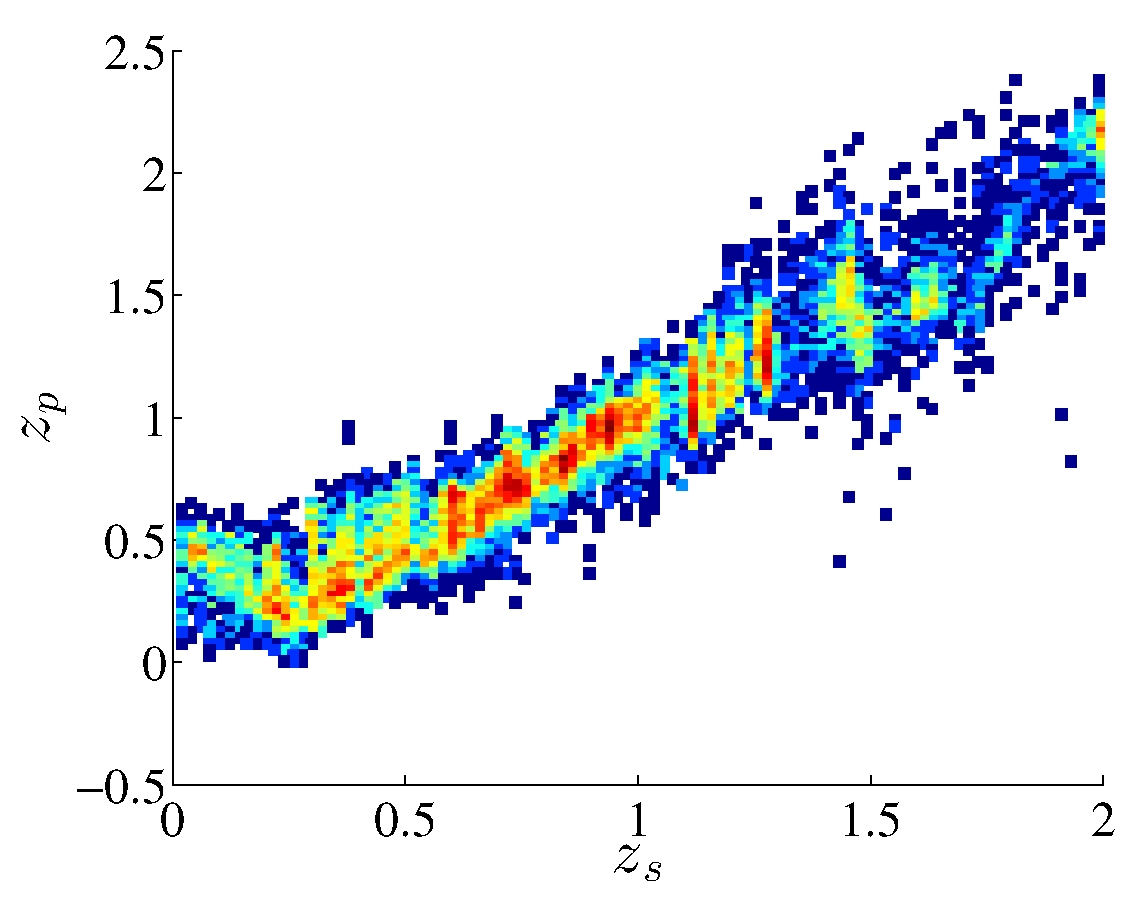
\includegraphics[width=\textwidth]{figures/GPGL.eps}
                \caption{GP-GL}
        \end{subfigure}
        ~
        \begin{subfigure}[b]{0.175\textwidth}
               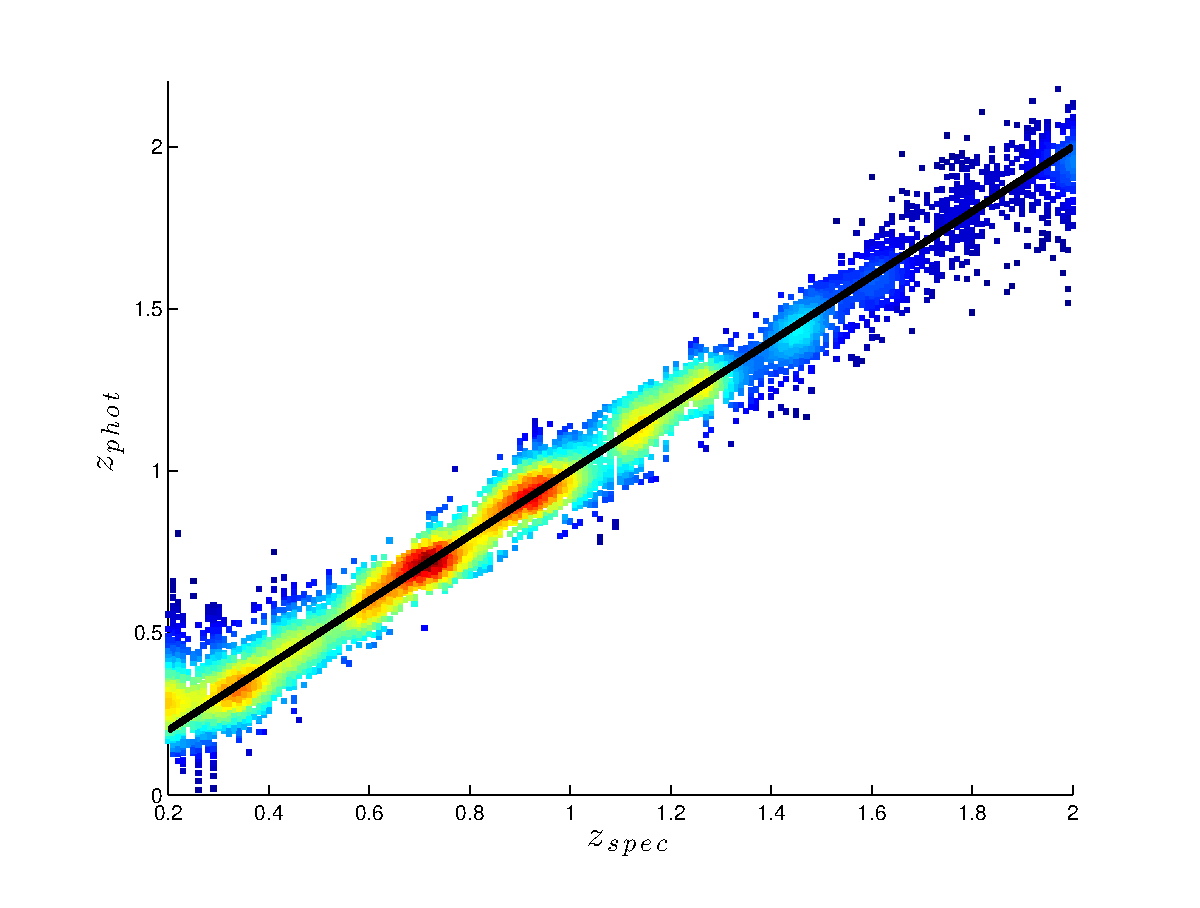
\includegraphics[width=\textwidth]{figures/GPVL.eps}
                \caption{GP-VL}
        \end{subfigure}
        ~
        \begin{subfigure}[b]{0.175\textwidth}
                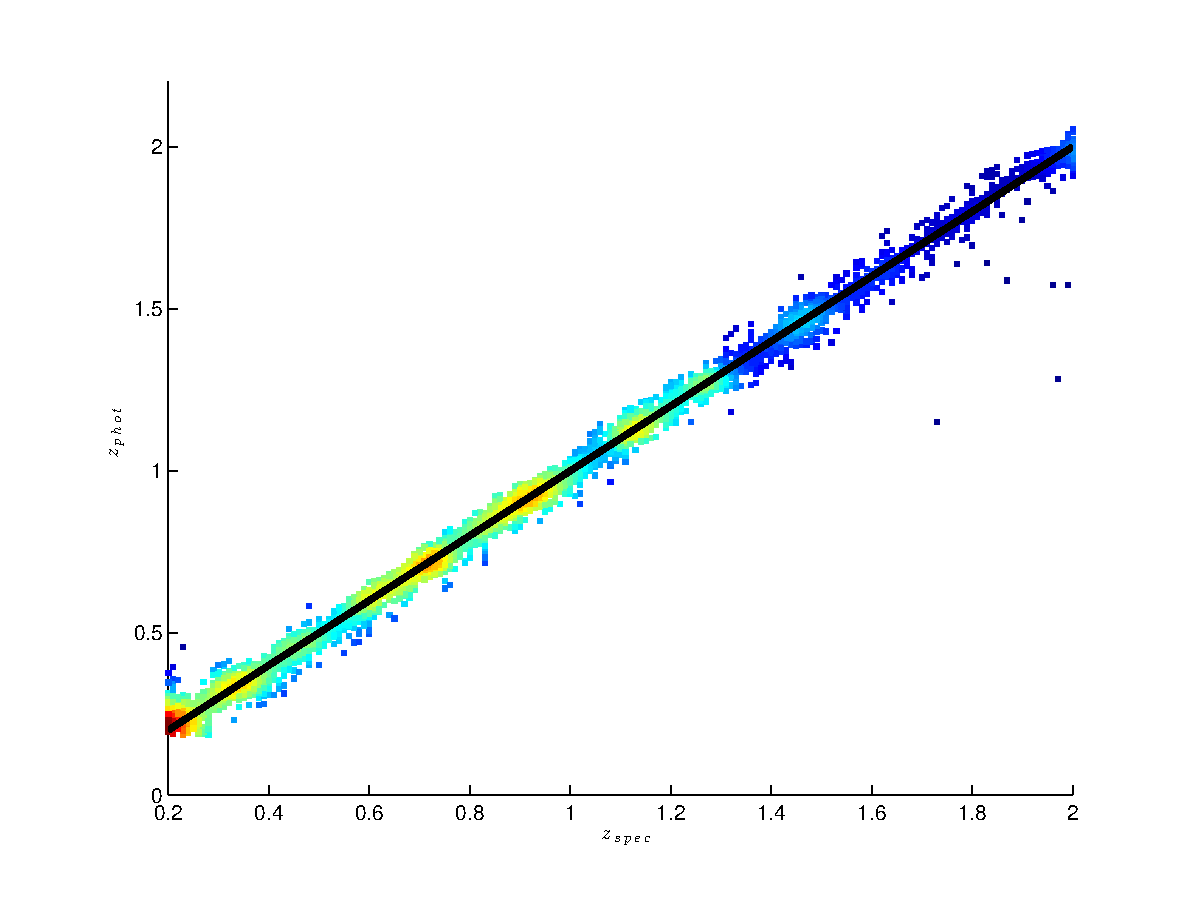
\includegraphics[width=\textwidth]{figures/GPVC.eps}
                \caption{GP-VC}
        \end{subfigure}
        
        \caption{Density scatter plots of the true $z_{spec}$ vs the predicted $z_{phot}$ for (a) ANN, (b) stableGP, (c) GP-GL, (d) GP-VL and (e) GP-VC using $m=10$ basis functions}
        \label{fig-experiment-1}
\end{figure*}

 \begin{table}
\caption{Performance measures for each algorithm trained using $m=10$ basis functions}
\begin{center}
  \begin{tabular}{| l | c | c | }
     				&	$\Delta z$	&	$\Delta z_{norm}$	\\	\hline
	ANN		&	0.0415		&	0.0251				\\	 
	stableGP	&	0.2138		&	0.1304				\\ 
	GP-GL		&	0.0679		&	0.0415				\\
	GP-VL		&	0.0595		&	0.0370				\\
	GP-VC		&	0.0233		&	0.0134				\\	\hline
  \end{tabular}
  \label{table-experiment-1}
\end{center}
\end{table}

\subsection{Prior Mean}

In this test, the extrapolation performance of the GP-VC model was tested using different prior means, namely a zero mean, a linear regression mean and a joint optimisation approach which learns the linear and non-linear features simultaneously by regularising the non-linear features more aggressively than linear features. To test this more effectively,  the models were trained using sources with $RIZ<23$ (36,244 objects) and tested on the unseen samples with $RIZ\ge23$, a similar test was also conducted using a split of $RIZ<22$ (15,067 objects). The results are reported in Table \ref{table-RIZ-splits} and the density scatter plots are shown for comparison in Figure \ref{fig-RIZ-splits}. The results from Table \ref{table-RIZ-splits} show that the ``Joint'' method consistently outperformed the other methods especially when trained with a small sample size as in the $RIZ<22$ case. The Linear regression prior was not always better than the zero mean prior in terms of performance measures, in the $RIZ<22$ case for example, but upon examining the density scatter plots in Figure \ref{fig-RIZ-splits}, the zero mean prior has more systematic and catastrophic errors.

 \begin{table}
\caption{Performance measures for each algorithm trained using $m=10$ basis functions}
\begin{center}
  \begin{tabular}{| l | c | c | c | c | }
  								& 	\multicolumn{2}{|c|}{$RIZ<23$}		& 	\multicolumn{2}{c}{$RIZ<22$} \\ \cline{2-5}
     	Prior						&	$\Delta z$	&	$\Delta z_{norm}$	&	$\Delta z$	&	$\Delta z_{norm}$	\\	\hline
	Zero						&	0.0807		&	0.0315				&	0.1436		&	0.0547					\\	 
	Linear Regression		&	0.0393		&	0.0188				&	0.1784		&	0.0689					\\ 
	Joint						&	0.0371		&	0.0167				&	0.0560		&	0.0264					\\	\hline
  \end{tabular}
  \label{table-RIZ-splits}
\end{center}
\end{table}

\begin{figure}
        \centering
        \begin{subfigure}[b]{0.3\columnwidth}
                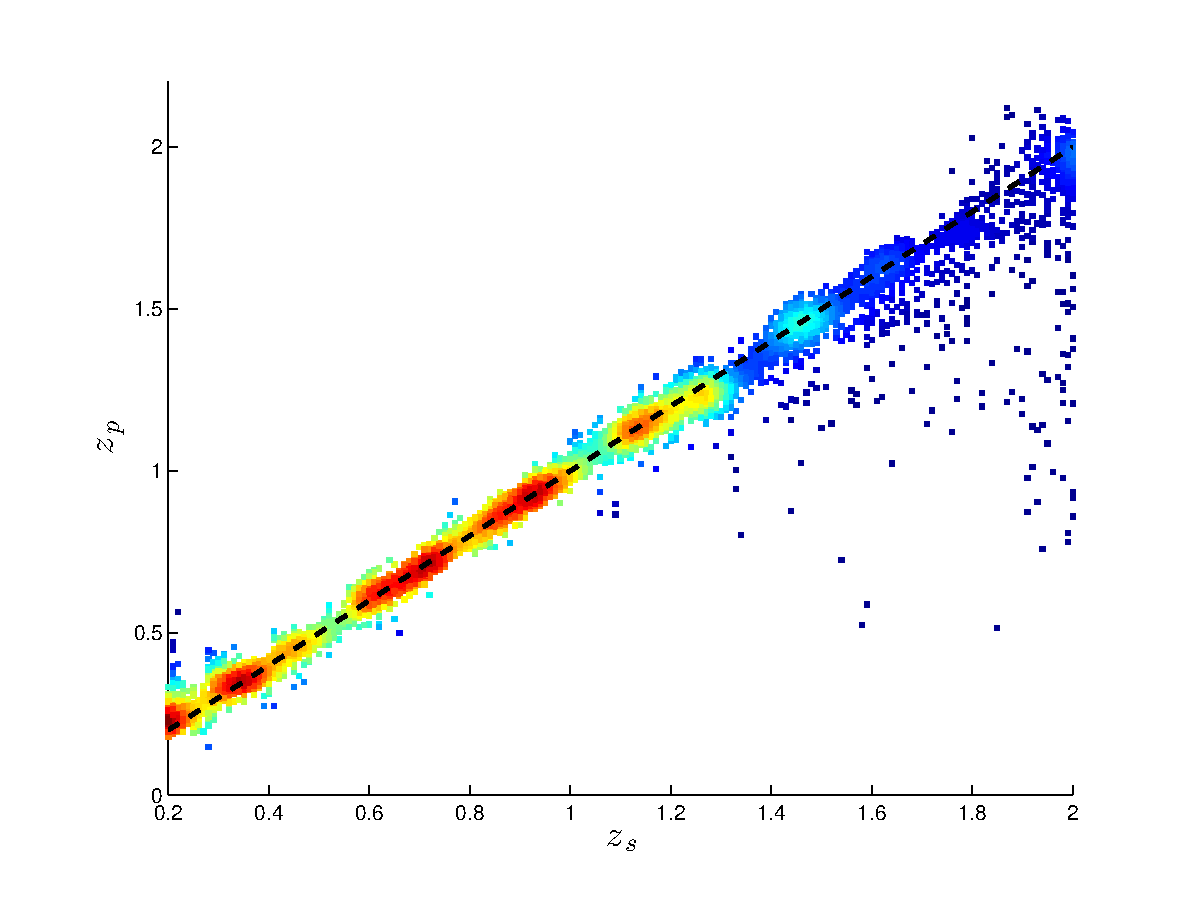
\includegraphics[width=\textwidth]{figures/23_0.eps}
        \end{subfigure}
        ~
        \begin{subfigure}[b]{0.3\columnwidth}
                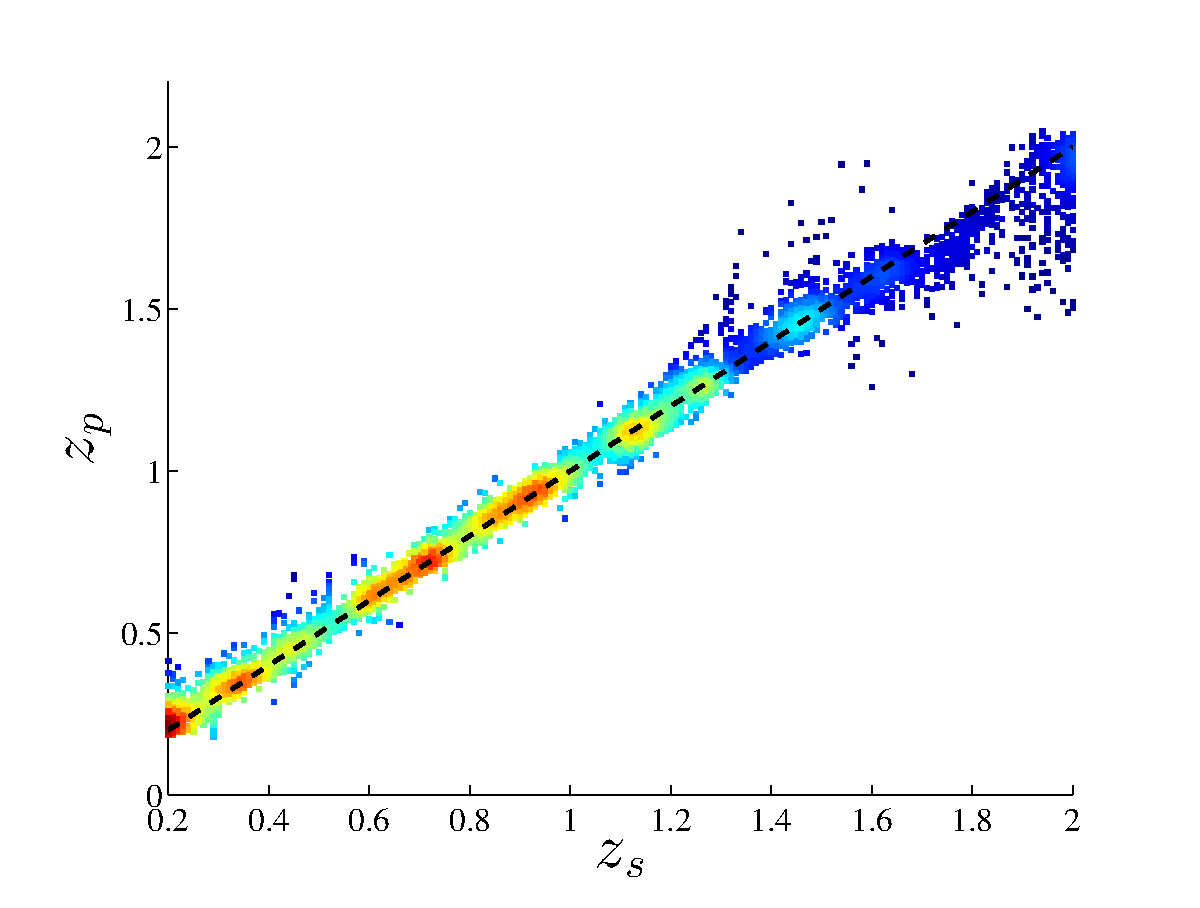
\includegraphics[width=\textwidth]{figures/23_L.eps}
        \end{subfigure}
        ~
        \begin{subfigure}[b]{0.3\columnwidth}
                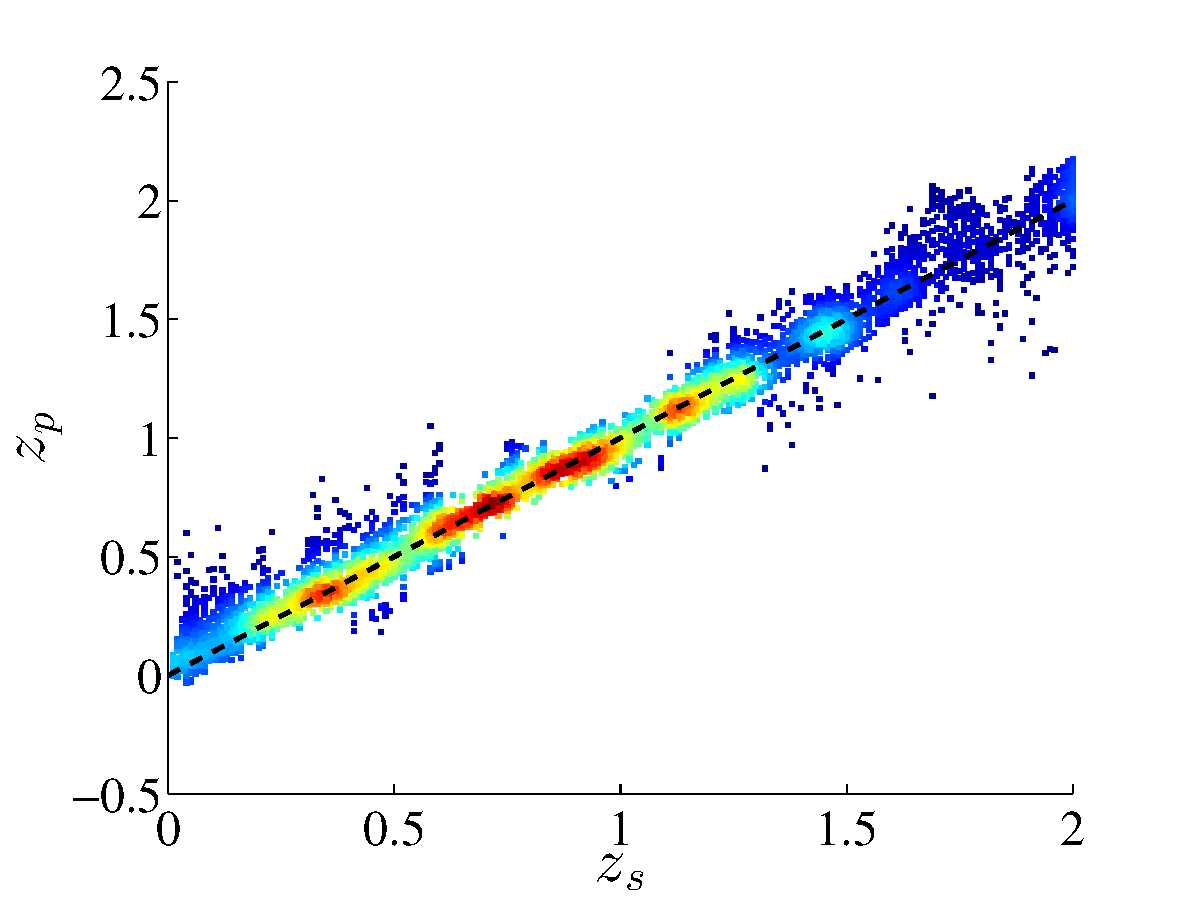
\includegraphics[width=\textwidth]{figures/23_J.eps}
        \end{subfigure}
        
       \begin{subfigure}[b]{0.3\columnwidth}
                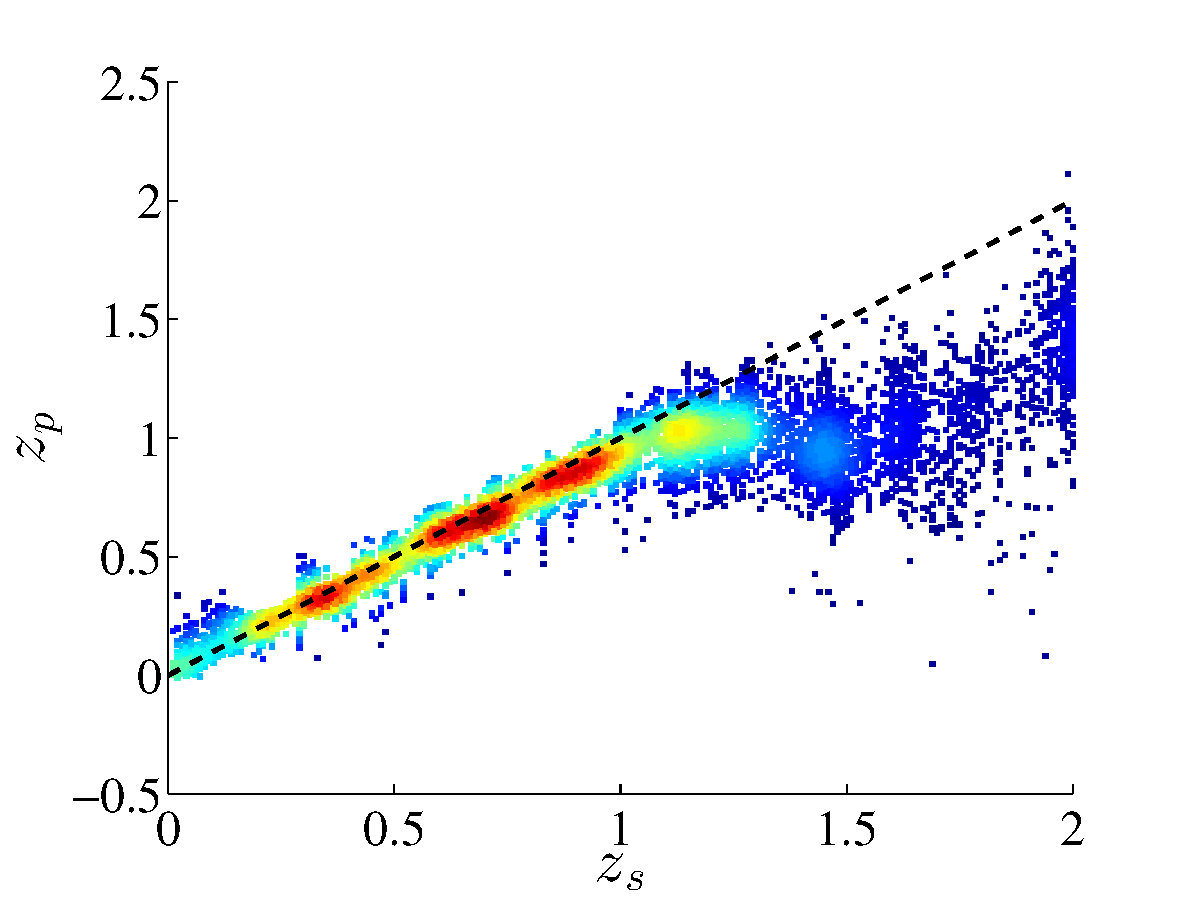
\includegraphics[width=\textwidth]{figures/22_0.eps}
                \caption{Zero mean}
        \end{subfigure}
        ~
        \begin{subfigure}[b]{0.3\columnwidth}
                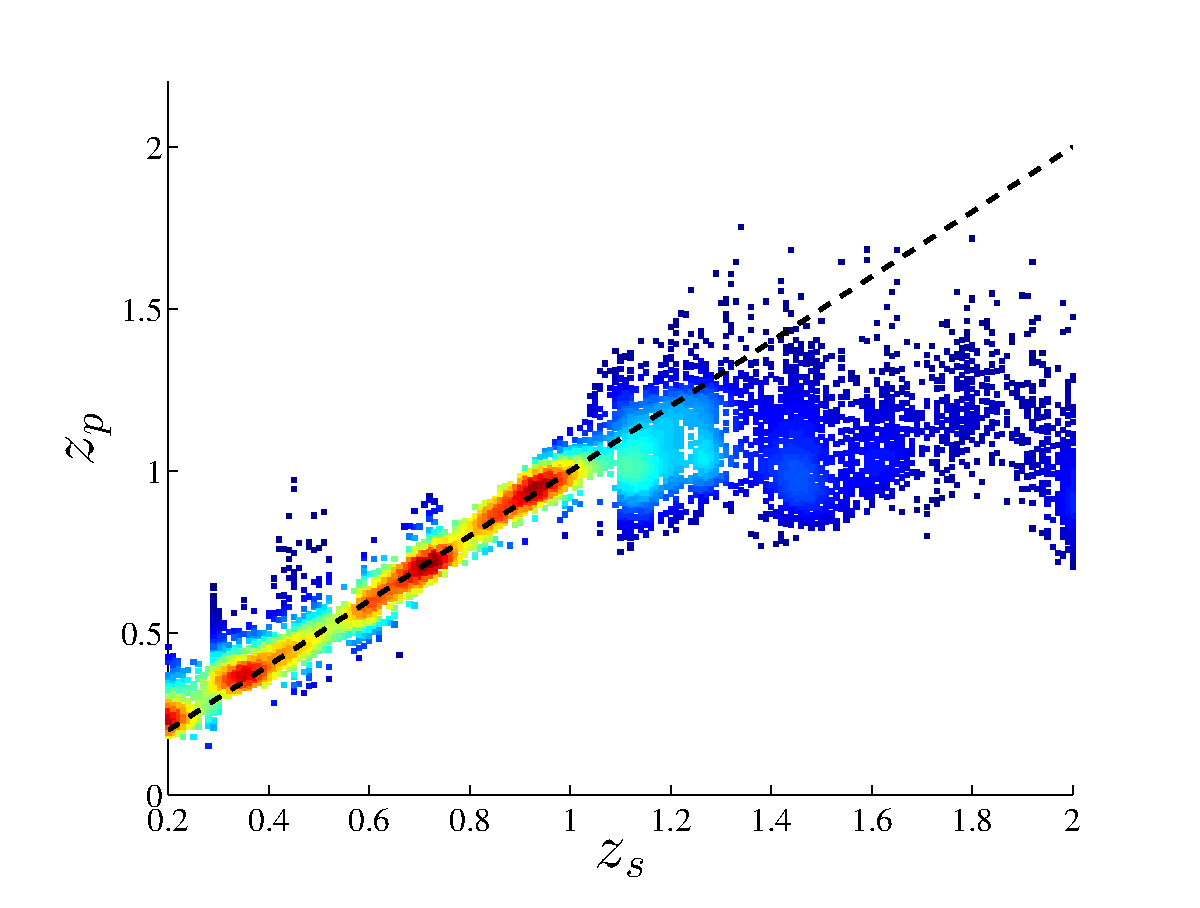
\includegraphics[width=\textwidth]{figures/22_L.eps}
                \caption{Linear}
        \end{subfigure}
        ~
        \begin{subfigure}[b]{0.3\columnwidth}
                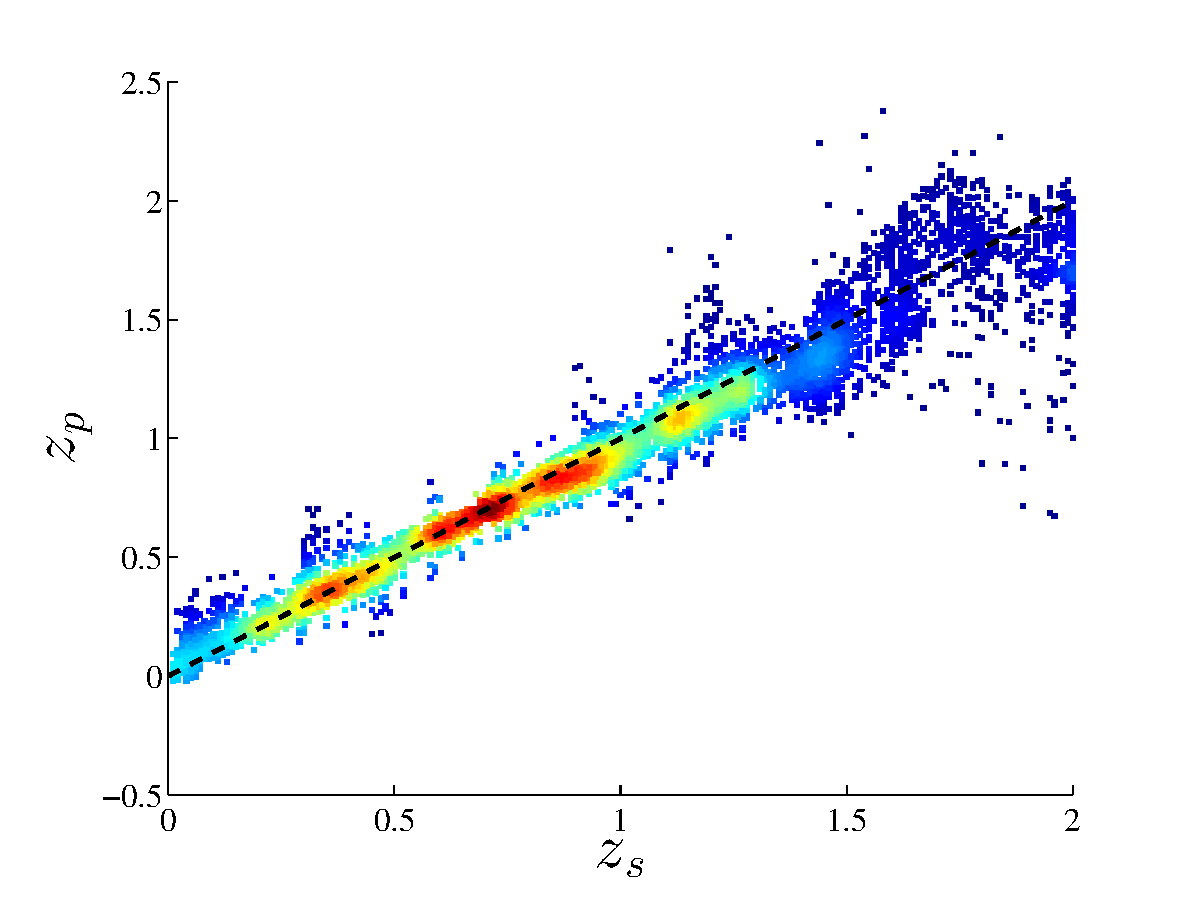
\includegraphics[width=\textwidth]{figures/22_J.eps}
                \caption{Joint}
        \end{subfigure}
        
        \caption{Density scatter plots of the true $z_{spec}$ vs the predicted $z_{phot}$ after training the GP-VC model with samples with $RIZ<23$ (top) and $RIZ<22$ (bottom) using $m=10$ basis functions with (a) zero mean, (b) linear regression and (c) joint linear and non-linear optimisation}
        \label{fig-RIZ-splits}
\end{figure}


\subsection{Weighted Samples}
In this experiment, a comparison between the cost sensitive learning and the normal sum of squares for the GP-VC model is presented. Two different weight configurations are tested, the first is to assign an error cost to each sample equals to $1/\left(1+z_{spec}\right)^{2}$ to directly target the Euclid mission requirement (Normalised), and the second experiment is to weigh each sample according to the frequency of their true redshift to insure balanced learning (Balanced).  Two additional measures are reported, the maximum $\Delta z$ and the maximum $\Delta z_{norm}$. The samples were grouped into bins of uniformly spaced intervals of 0.01, the mean error and the 1 standard deviation confidence bars are shown in Figure \ref{fig-normal} for the normal weighting scheme and Figure \ref{fig-balanced} shows the results of the balanced training. The results from the figures show that the cost sensitive learning is more consistent across the redshift range as oppose to the normal sum of squares, especially in the high redshift regions were there is less data the confidence intervals are considerably smaller. The performance comparison for the normal, balanced and normalised training are summarised in Table \ref{table-normal-balanced}. Balanced training showed a better generalisation performance, as it out performed the normal sum of squares objective on the test set and has lower maximum errors.

\begin{figure}
        \centering
        \begin{subfigure}[b]{\columnwidth}
                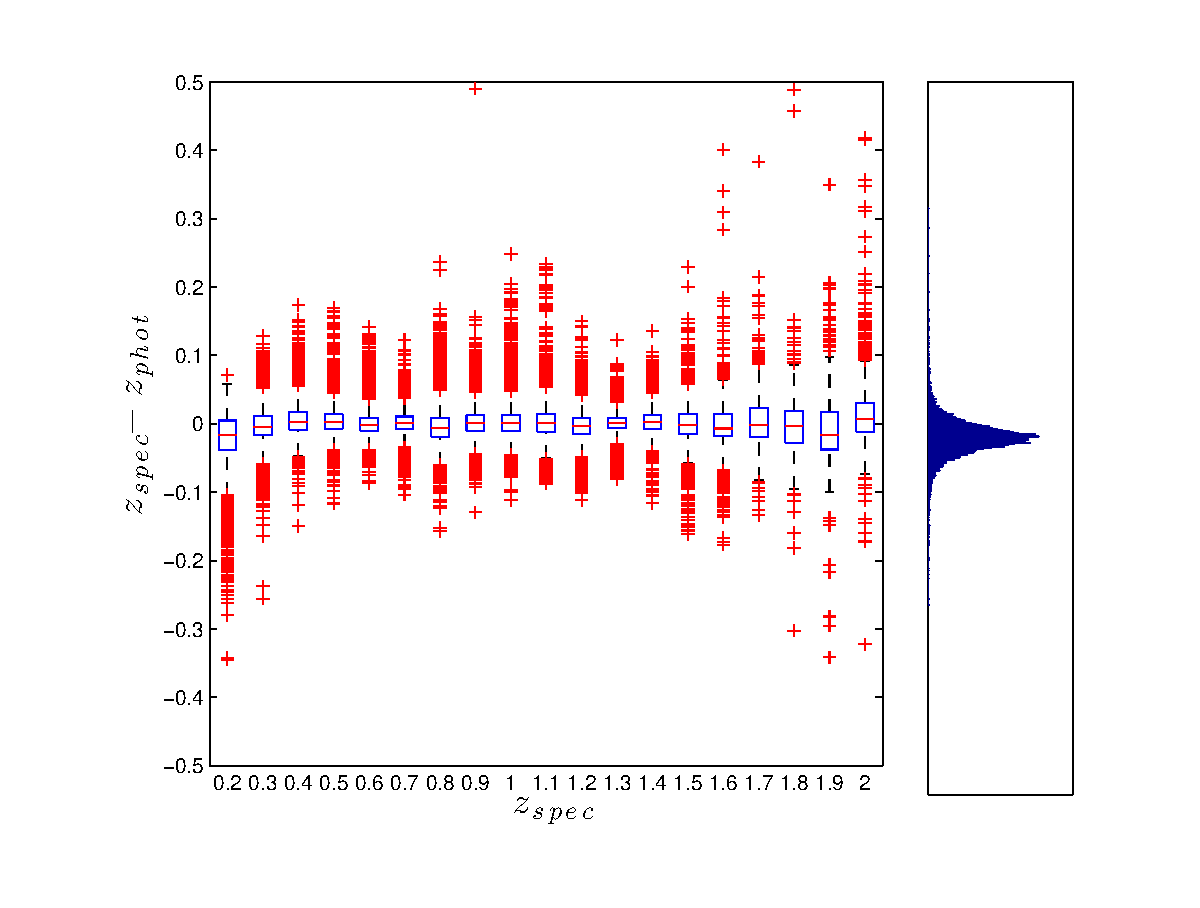
\includegraphics[width=\textwidth]{figures/Zspec-Zphot_normal.eps}
                \caption{Normal}
                \label{fig-normal}
        \end{subfigure}
	
        \begin{subfigure}[b]{\columnwidth}
                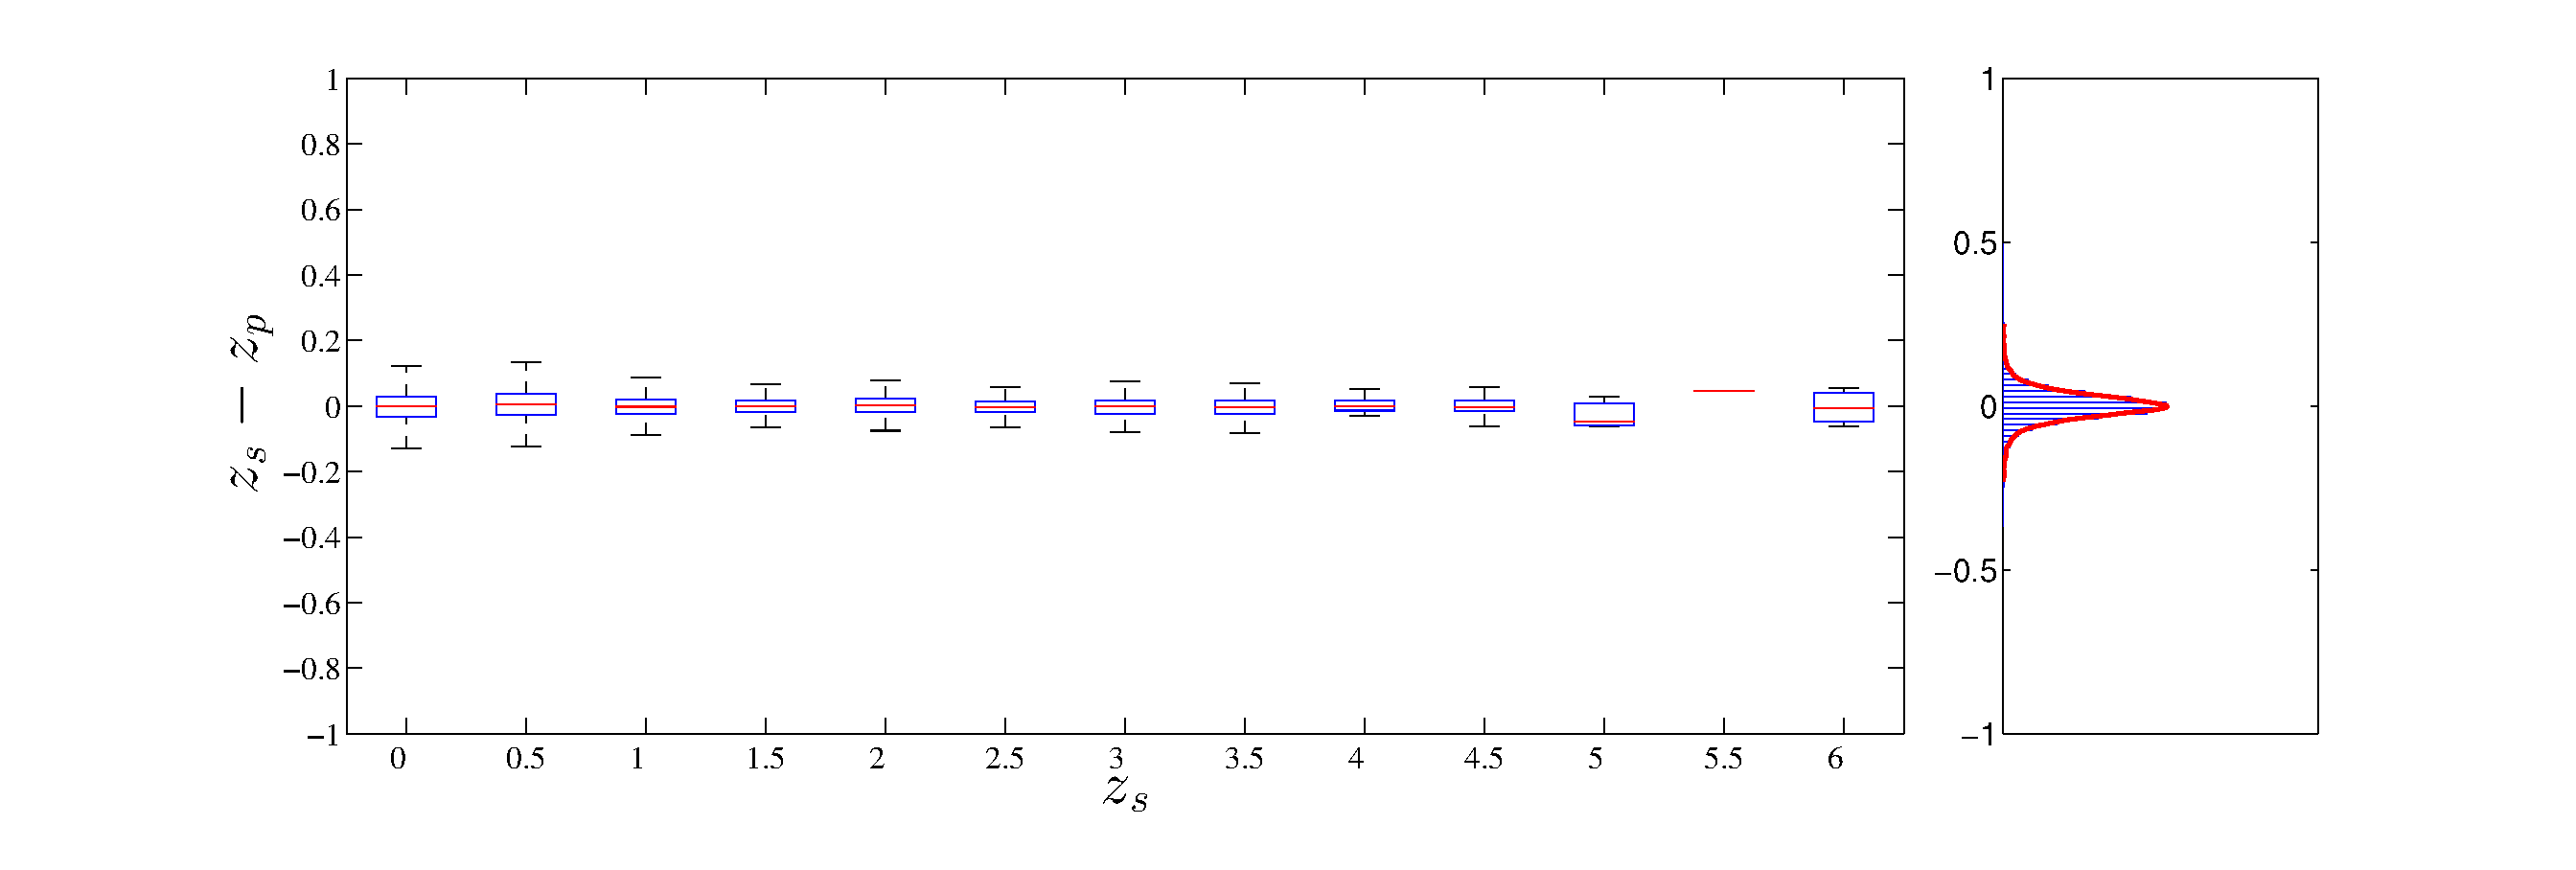
\includegraphics[width=\textwidth]{figures/Zspec-Zphot_balanced.eps}
                \caption{Balanced}
                \label{fig-balanced}
        \end{subfigure}
        
       \caption{The error as a function of redshift for the (a) normal sum of squared errors and (b) for the balanced cost sensitive learning for the GV-VC model when trained with $m=10$ basis functions}
	\label{fig-normal-balanced}
\end{figure}

 \begin{table}
\caption{Performance measures of training the GP-VC model using $m=10$ basis functions and different weighting schemes}
\begin{center}
  \begin{tabular}{| l | c | c | c | c |}
     				&	$\Delta z$	&	$max(\Delta z)$		&	$\Delta z_{norm}$		&	$max(\Delta z_{norm})$	\\	\hline
	Normal		&	0.0233		&	0.6879				&	0.0134				&	0.2316					\\	 
	Balanced	&	0.0215		&	0.3466				&	0.0136				&	0.2818					\\ 
	Normalised	&	0.0216		&	0..2695				&	0.0119				&	0.2191					\\	\hline
  \end{tabular}
  \label{table-normal-balanced}
\end{center}
\end{table}

\subsection{Kernel Analysis}
In this experiment, we study the resulted kernels and their learned basis functions. Figure \ref{fig-kernel-activations} shows the patterns for the top five kernels after training GP-VC with $m=10$ basis functions and their activation as a function of redshift. The kernels were ranked based on the difference between the maximum and minimum mean activations per bin (uniformly spaced by 0.01).

\textit{COMMENT: Is there anything interesting to say here?}

\begin{figure*}
        \centering
        
        \begin{subfigure}[b]{0.175\textwidth}
                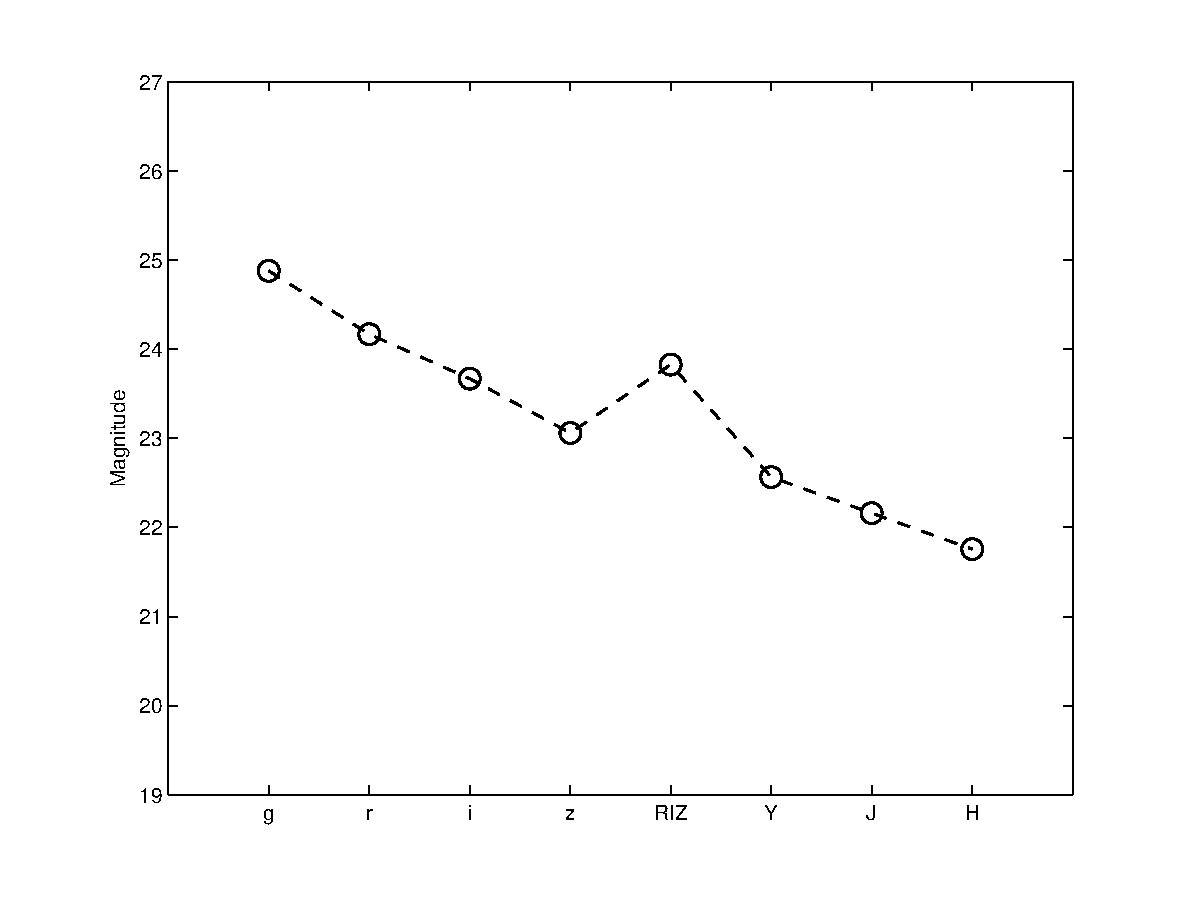
\includegraphics[width=\textwidth]{figures/basis_01.eps}
        \end{subfigure}
	~
        \begin{subfigure}[b]{0.175\textwidth}
                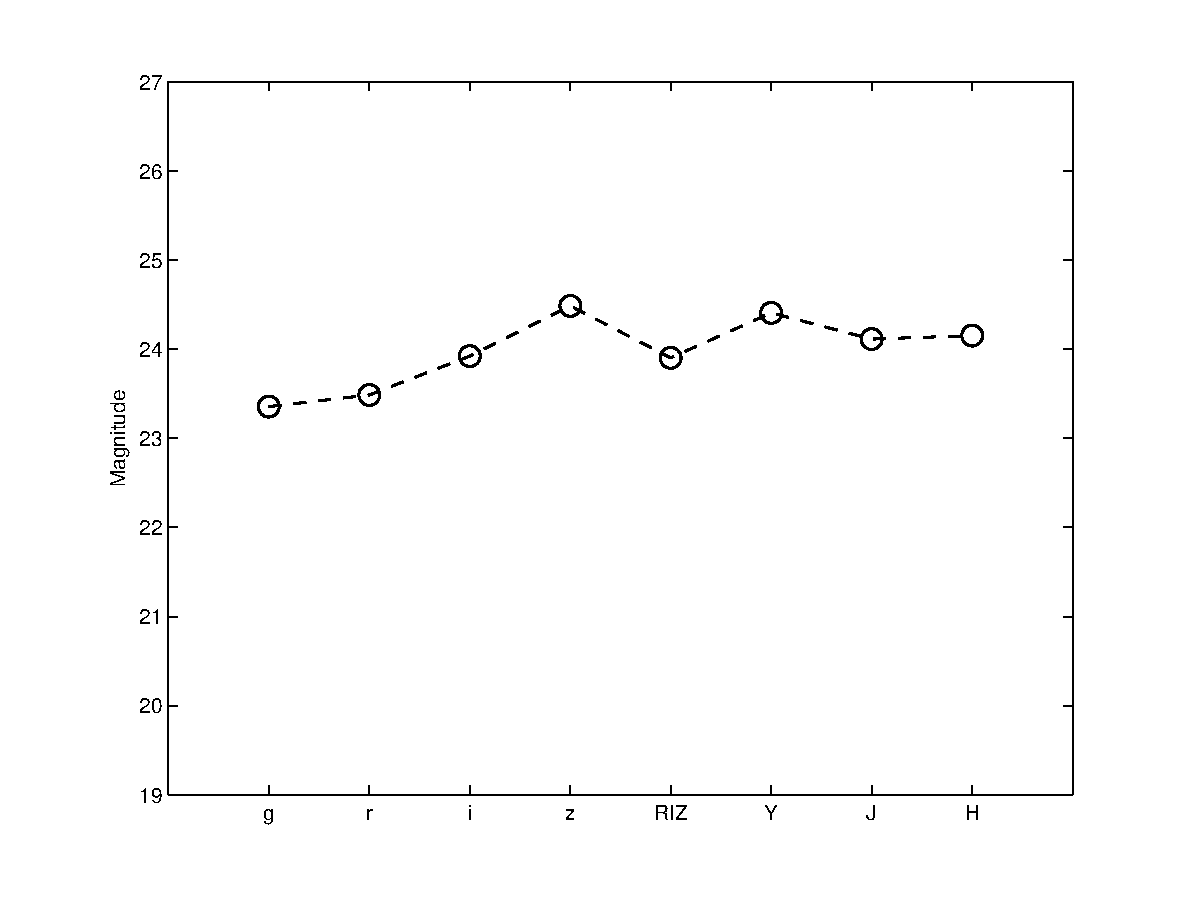
\includegraphics[width=\textwidth]{figures/basis_02.eps}
        \end{subfigure}
        ~
        \begin{subfigure}[b]{0.175\textwidth}
                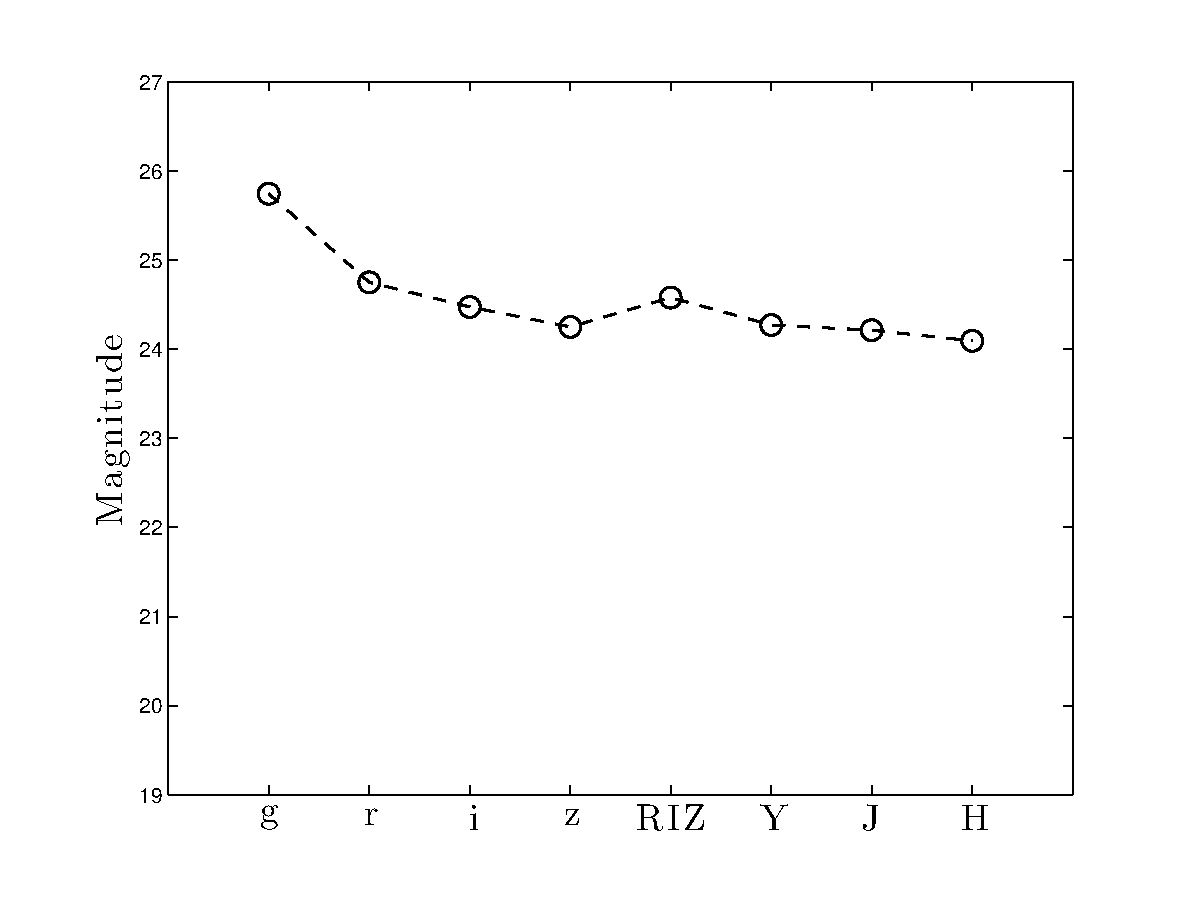
\includegraphics[width=\textwidth]{figures/basis_03.eps}
        \end{subfigure}
        ~
        \begin{subfigure}[b]{0.175\textwidth}
                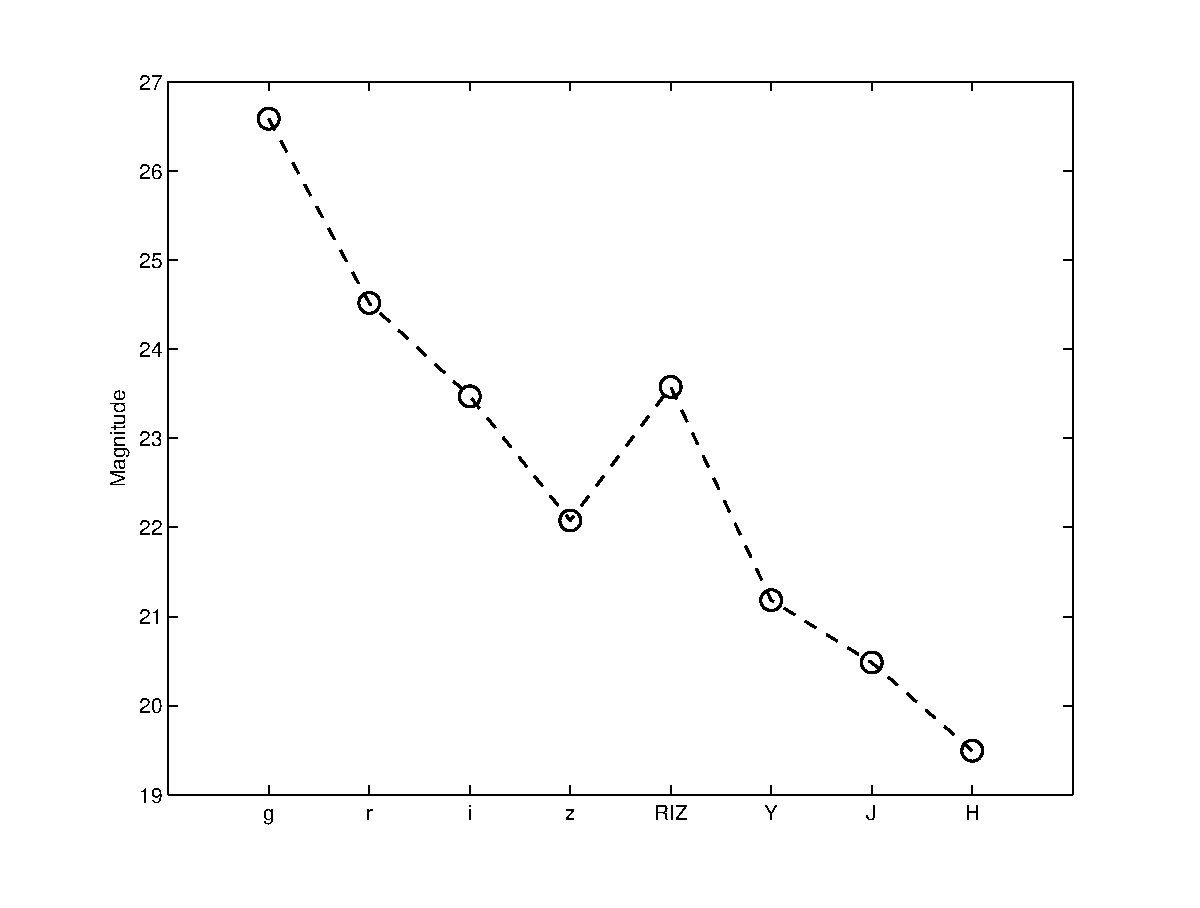
\includegraphics[width=\textwidth]{figures/basis_04.eps}
        \end{subfigure}
        ~
        \begin{subfigure}[b]{0.175\textwidth}
                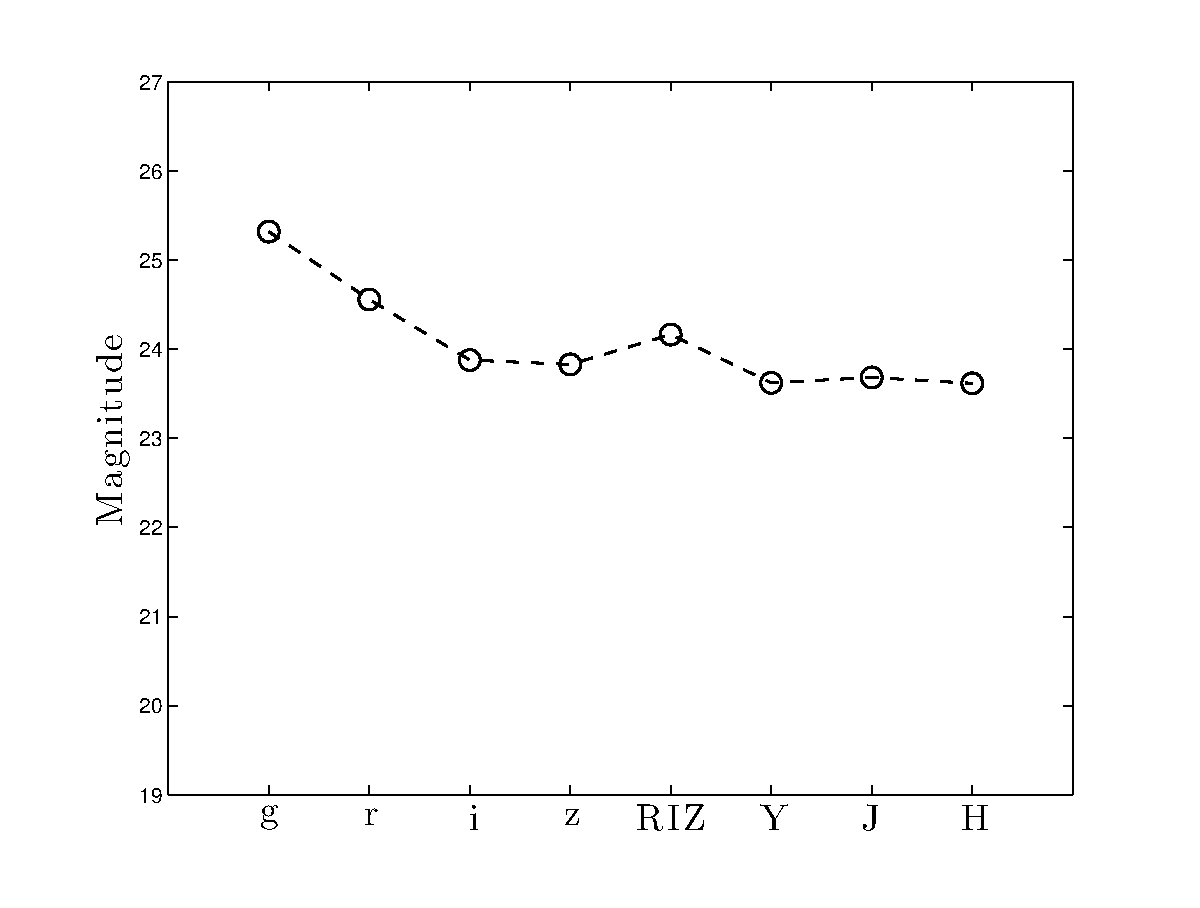
\includegraphics[width=\textwidth]{figures/basis_05.eps}
        \end{subfigure}

        
        \begin{subfigure}[b]{0.175\textwidth}
                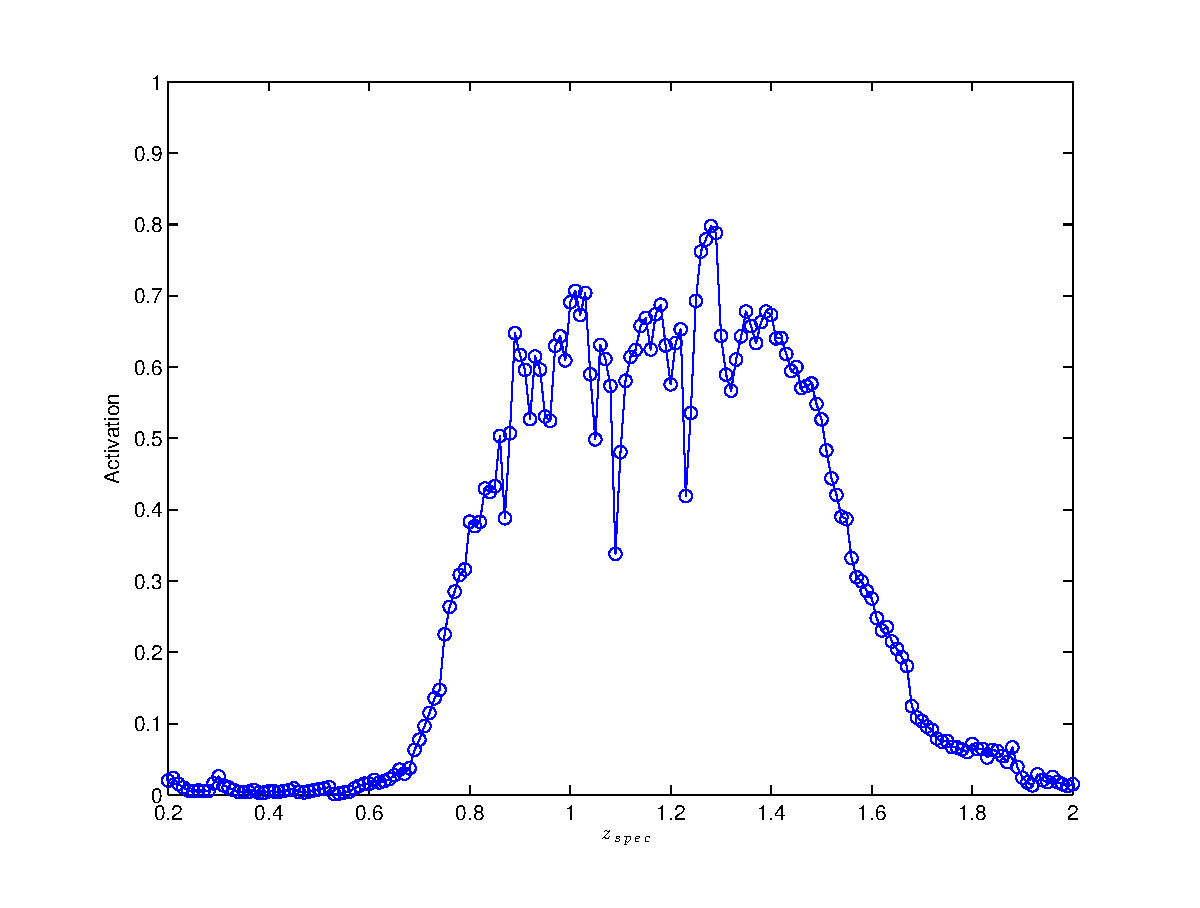
\includegraphics[width=\textwidth]{figures/activation_01.eps}
        \end{subfigure}
	~
        \begin{subfigure}[b]{0.175\textwidth}
                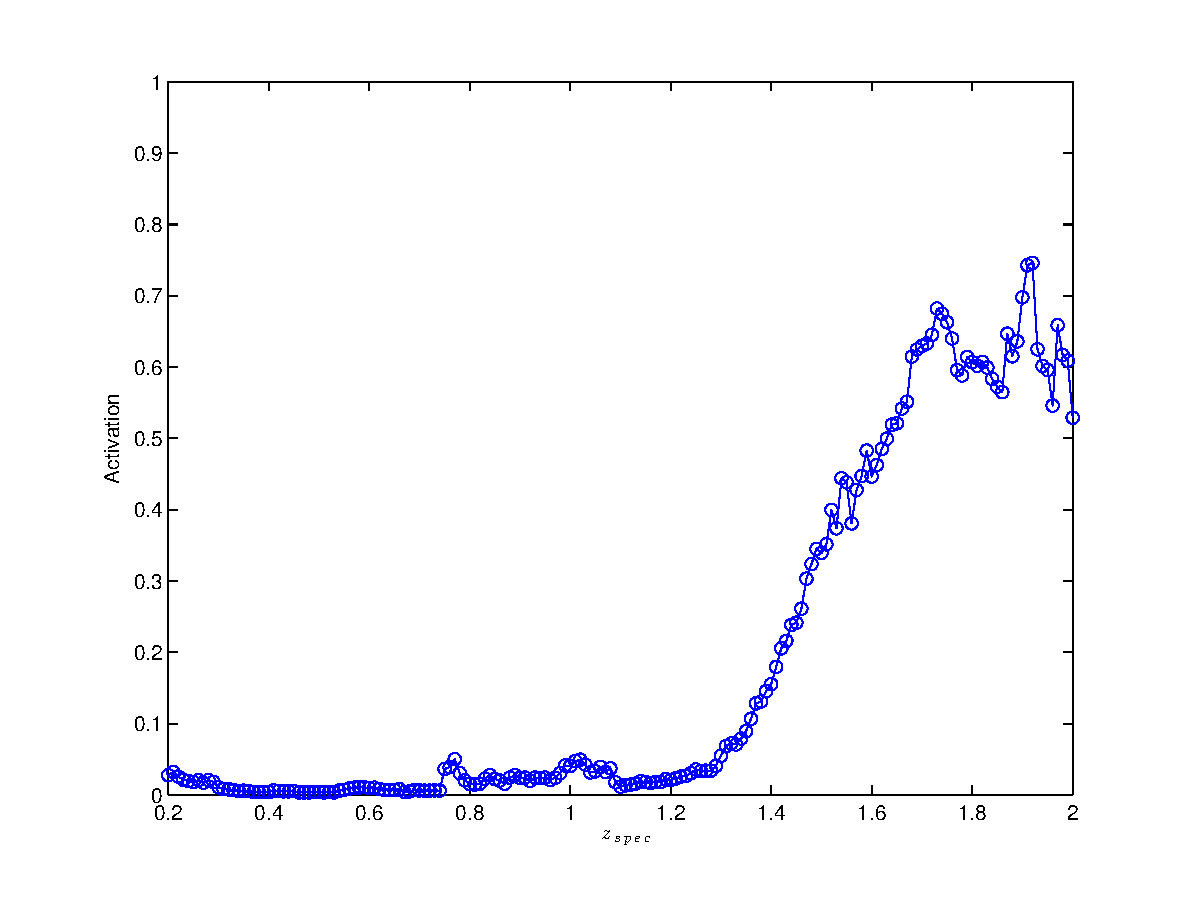
\includegraphics[width=\textwidth]{figures/activation_02.eps}
        \end{subfigure}
        ~
        \begin{subfigure}[b]{0.175\textwidth}
                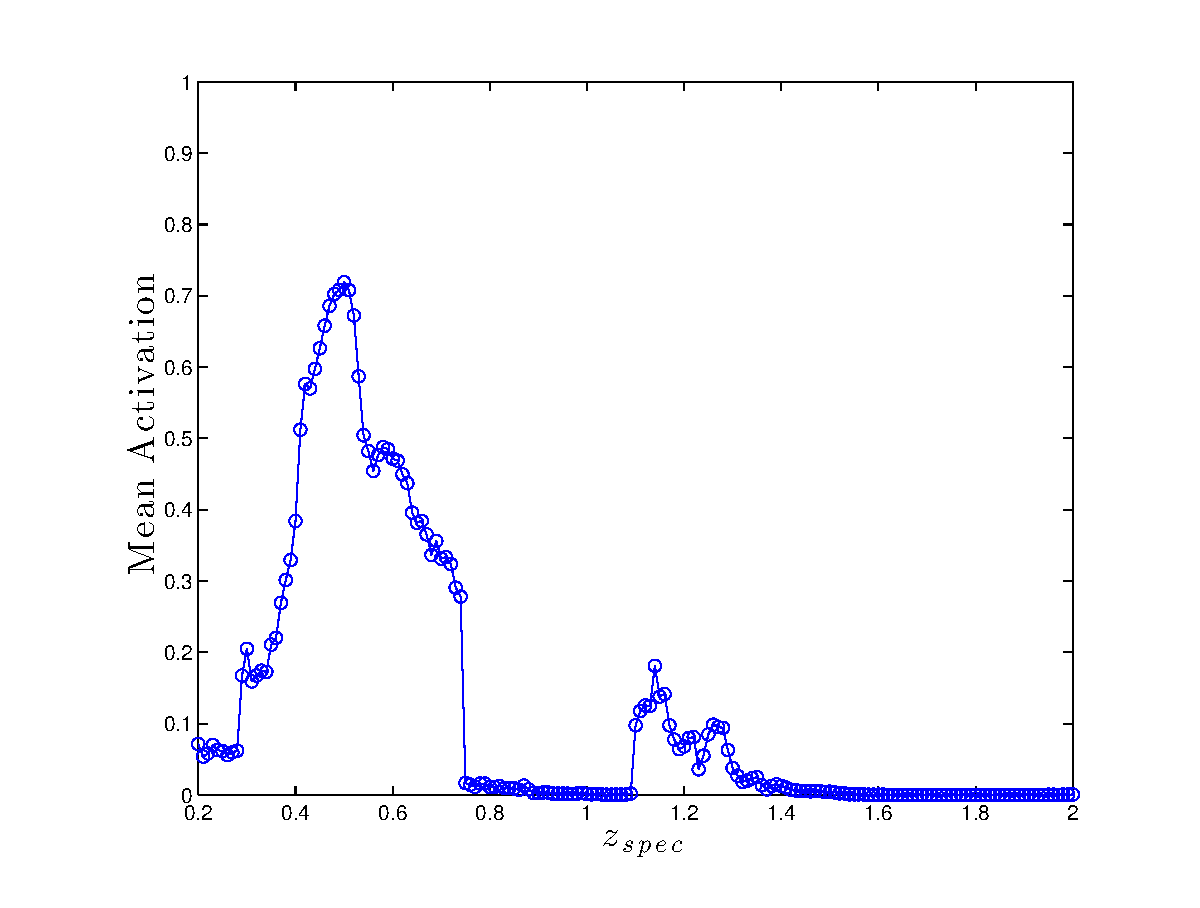
\includegraphics[width=\textwidth]{figures/activation_03.eps}
        \end{subfigure}
        ~
        \begin{subfigure}[b]{0.175\textwidth}
                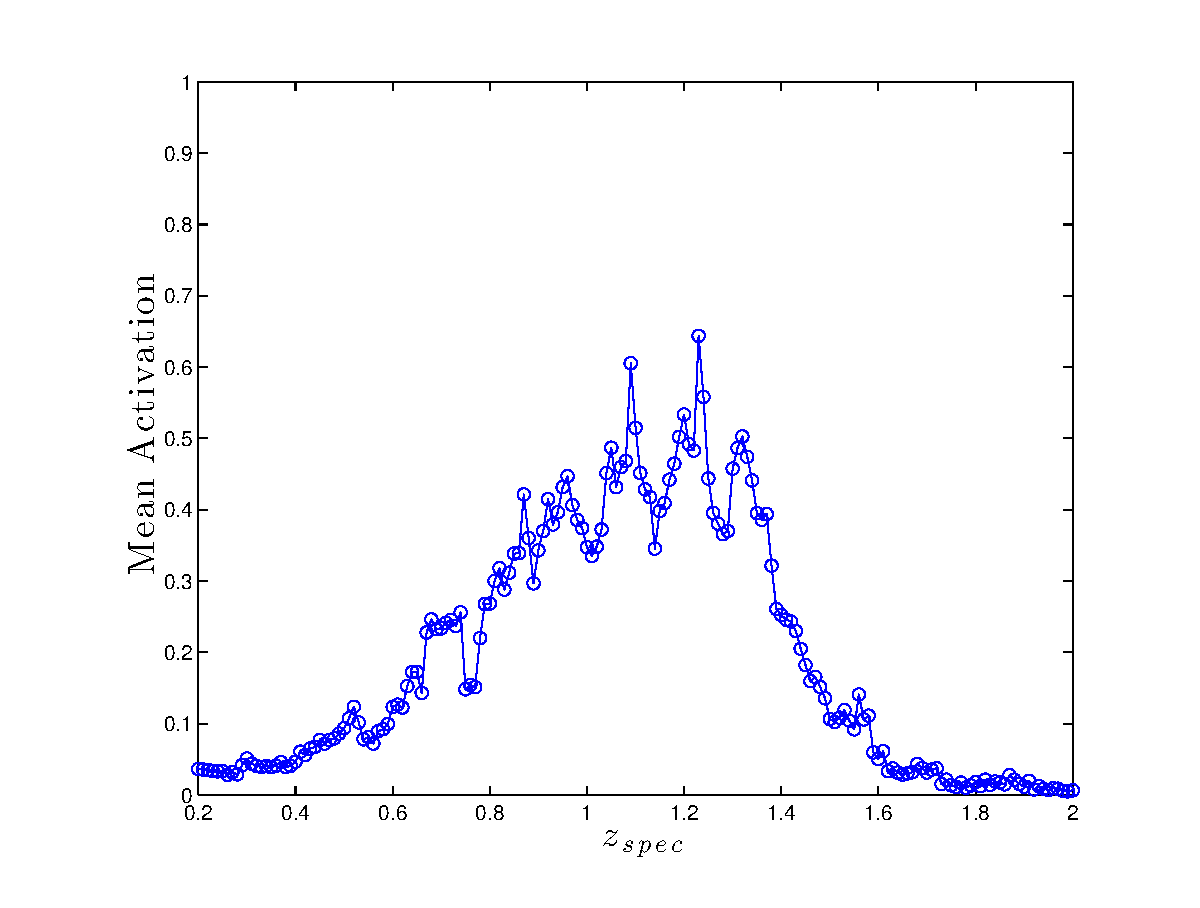
\includegraphics[width=\textwidth]{figures/activation_04.eps}
        \end{subfigure}
        ~
        \begin{subfigure}[b]{0.175\textwidth}
                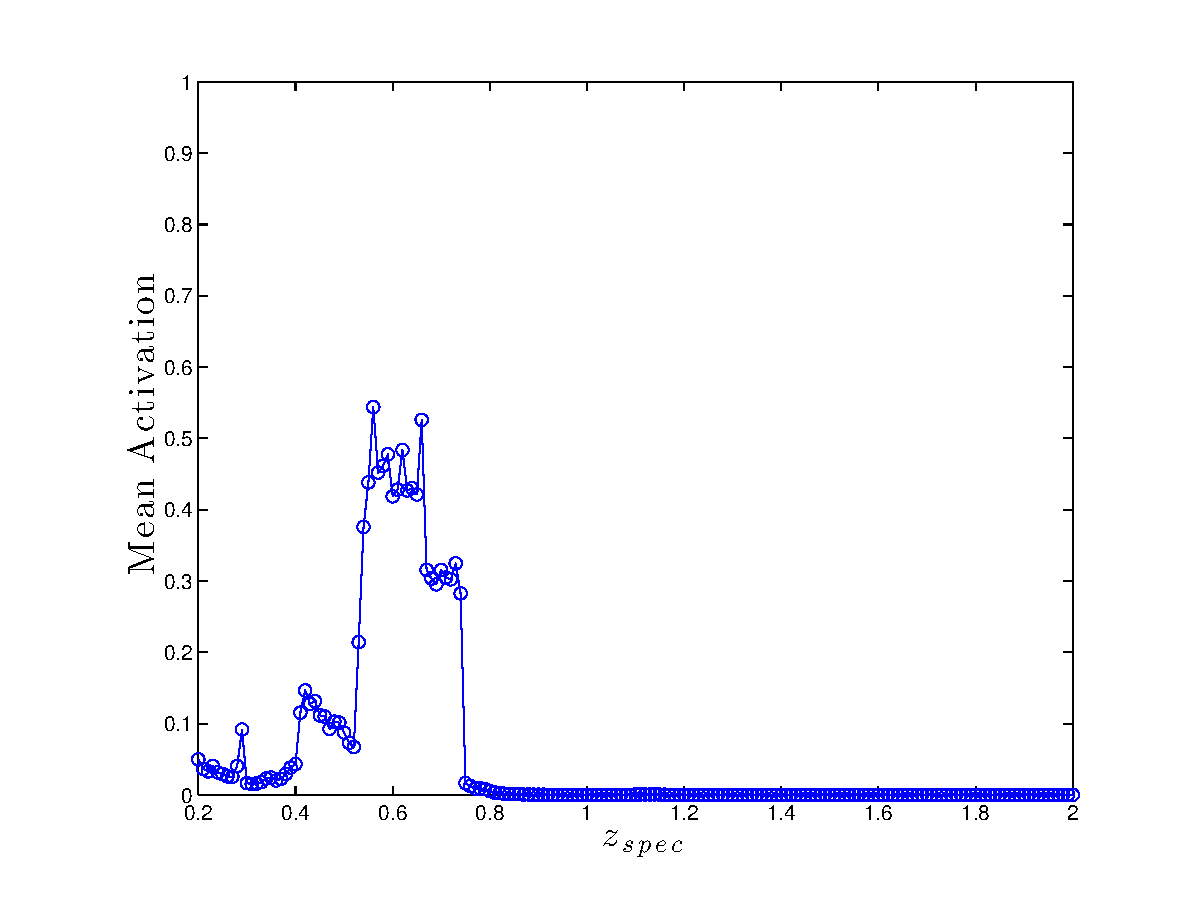
\includegraphics[width=\textwidth]{figures/activation_05.eps}
        \end{subfigure}
        
       \caption{The top 5 basis (top) and their corresponding average activation as a function of redshift (bottom) after training GP-VC with $m=10$ basis functions}
	\label{fig-kernel-activations}
\end{figure*}

\subsection{Size of the basis set}
In this test, all the models are cross compared by varying the number of basis functions $m$ to 10, 25, 50, 100 and 200. The plot of the $\Delta z$ as a function of $m$ is shown in Figure \ref{fig-rmses}. The stable GP showed the worst performance across the board, especially when the number of basis was low, while GP-VC on the other hand consistently outperformed the rest and most significantly when trained with a few number of basis. ANN outperformed GP-GL and GP-VL, but it did not scale well with complexity as it converged around $m=100$. All the models were trained using a sum of squares objective with no cost sensitive learning or prior mean function. To determine the best number of basis functions the models were scored using the Bayesian Information Criterion (BIC) \citep{schwarz1978}  that takes into account both the accuracy and the complexity of each model Eq. \eqref{eq-bic} and the results are reported in Figure \ref{fig-bic}. The scores are plotted against the number of basis functions for the sake of visualisation, but the values were scored based on the number of free parameters, or the degree of freedom $\mathcal{D}$. The GP-VC approach had the best BIC score using the least number of basis functions ($m=25$).

\begin{equation}
\label{eq-bic}
BIC = n \cdot \log(\Delta z)+\mathcal{D}\cdot \log(n)
\end{equation}

The final GP-VC model to target the Euclid Space Mission was trained with $m=200$ basis functions normalised, balanced and with a joint mean optimisation reached a $\Delta z_{norm}=0.003$ and a  $max(\Delta z_{norm})=0.044$ and the scatter plot for the final model is shown in Figure \ref{fig-final-model}.

\begin{figure}
        \centering
        
        \begin{subfigure}[b]{0.45\textwidth}
                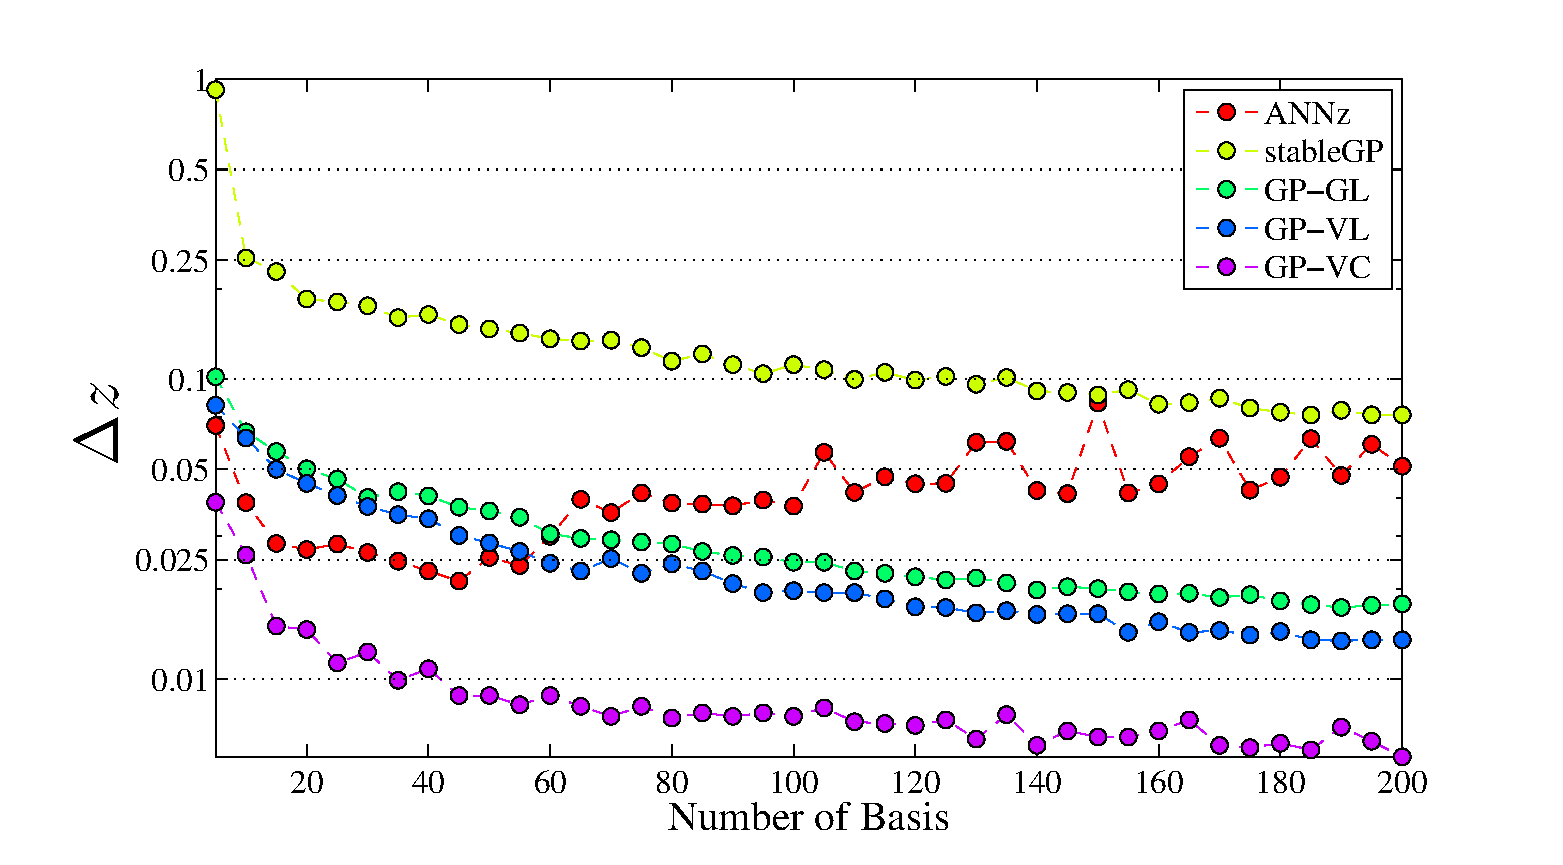
\includegraphics[width=\textwidth]{figures/different-basis.eps}
                 \caption{Root Mean Squared Error.} 
                 \label{fig-rmses}
        \end{subfigure}
	~
       \begin{subfigure}[b]{0.45\textwidth}
                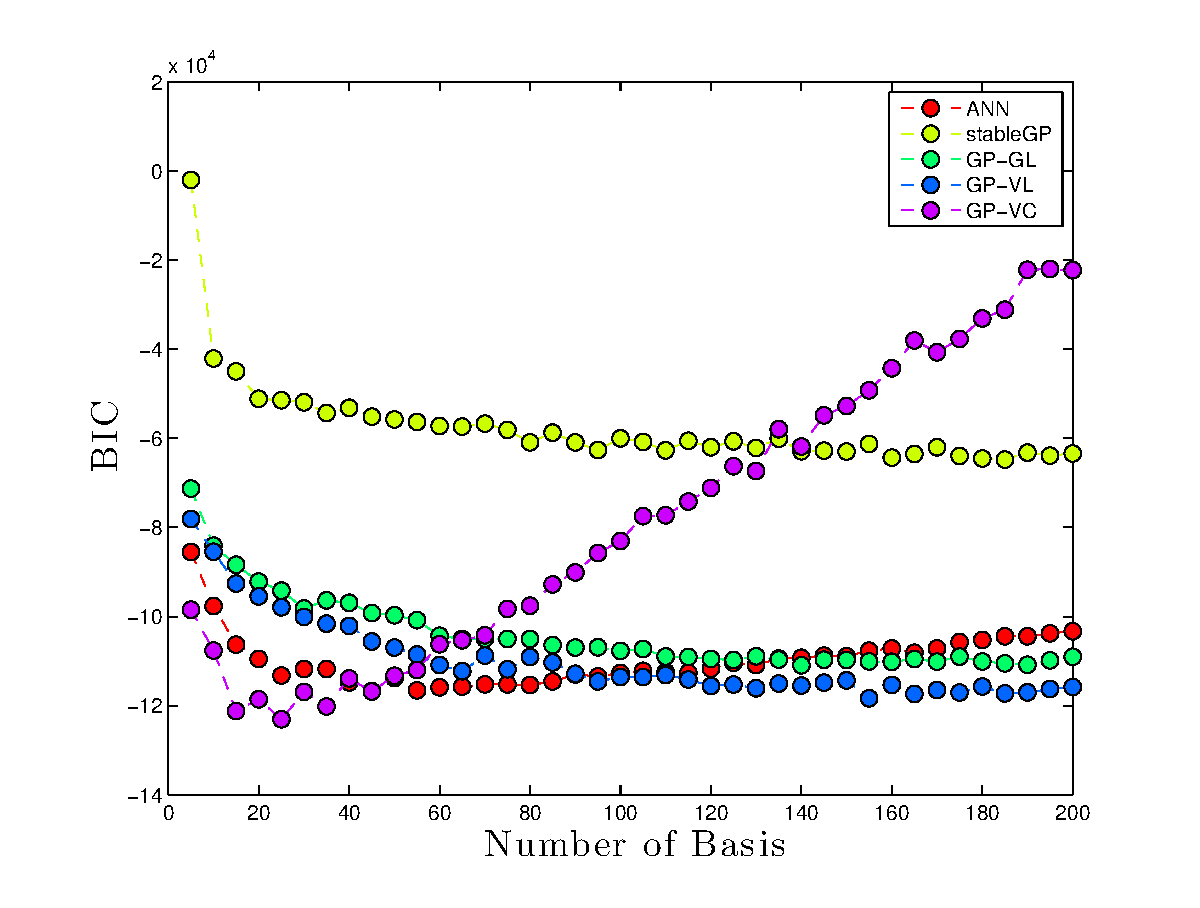
\includegraphics[width=\textwidth]{figures/BIC.eps}
                 \caption{Bayesian Information Criterion.} 
                 \label{fig-bic}
        \end{subfigure}

       \caption{The root mean squares (a) and the BIC scores (b) as a function of $m$ for all the models.} 
	
\end{figure}

\begin{figure}
       \centering
        \includegraphics[width=\columnwidth]{figures/final-model.eps}
        \caption{The density scatter plot for the final GP-VC model trained using $m=200$ basis functions with a jointly optimised linear mean function, a balanced and normalised weights. } 
       \label{fig-final-model}
\end{figure}


\section{Conclusion}
In this paper a sparse gaussian process framework was presented and applied to photometric redshift estimation. The framework was able to out perform Artificial Neural Networks and sparse gaussian processes with a global set of hyper-parameters. The performance increase is attributed to the handling of distribution bias via a weighting scheme integrated as part of the optimisation objective, parameterising each basis function with different covariances, and integrating the learning of the prior mean function to enhance the extrapolation performance of the model. The methods were applied to a simulated data set and the proposed approach consistently outperformed the other models on all measures while maintaining a low ration of model complexity to accuracy as scored by the Bayesian Information Criterion.
\label{sec-conclusion}

\footnotesize{
\bibliographystyle{mn2e}
\bibliography{sources}	
}

\end{document}
